% !TeX spellcheck = fr_FR
%%%%%%%%%%%%%%%%%%%%%%%%%%%%%%%%%%%%%%%%%%%%%%%%%%%%%%%%%%%%%%%%%%%%%%%%%%%%%%%%
%%                                                                             %
%% HEPIA BACHELOR THESIS LATEX TEMPLATE                                        %
%% version 0.10 - 2020/04/22                                                    %
%%                                                                             %
%%%%%%%%%%%%%%%%%%%%%%%%%%%%%%%%%%%%%%%%%%%%%%%%%%%%%%%%%%%%%%%%%%%%%%%%%%%%%%%%
% Ensure no option clash for url package; hyperref will manage links
\RequirePackage{url}
\documentclass[12pt
%% UNCOMMENT THE LINE BELOW TO HAVE CHAPTER STARTING ON THE RIGHT PAGE
%			,twoside, openright
			]{report} %% should use memoir documentclass
%%%%%%%%%%%%%%%%%%%%%%%%%%%%%%%%%%%%%%%%%%%%%%%%%%%%%%%%%%%%%%%%%%%%%%%%%%%%%%%%
%%                                                                             %
%% HEPIA BACHELOR THESIS LATEX TEMPLATE                                        %
%% version 0.10 - 2020/04/25                                                    %
%%                                                                             %
%%%%%%%%%%%%%%%%%%%%%%%%%%%%%%%%%%%%%%%%%%%%%%%%%%%%%%%%%%%%%%%%%%%%%%%%%%%%%%%%

\usepackage[T1]{fontenc}
\usepackage[utf8]{inputenc}
\usepackage[french]{babel}
\usepackage[cm]
			{fullpage}	% Set margins to full page
\usepackage[a4paper,includeheadfoot,margin=2.5cm]{geometry}
%\usepackage[a4paper,includehead,includefoot,top=2.1cm,bottom=2.5cm,right=2.5cm,left=2.5cm]{geometry}
\usepackage{lmodern}	% latin Modern font (FALLBACK FONT)
% biblatex removed - using custom reference system
\usepackage{caption}
\usepackage{csquotes}
\captionsetup{labelfont=sc}
% You can change names of table and figure here
\def\frenchtablename{Tableau} 
\def\frenchfigurename{Illustration} 

\usepackage{float}
\usepackage{tikz}		% Image and drawing related package - TITLE PAGE
\usepackage{setspace}	% Custom spacing package            - TITLE PAGE
\usepackage{array}		% Array related package				- TITLE PAGE
\usepackage{helvet}		% Helvetica font ~ Arial			- TITLE PAGE
\usepackage{mathptmx}	% Times font ~ Times New Roman
\usepackage{subcaption}
\usepackage{placeins}
\usepackage{carlito}	% Calibri replacement font
\usepackage[scaled=0.85]
			{beramono}	% Vera mononspace {fvm}

%% This defines the default sans serif, roman and monospace fonts
\renewcommand{\sfdefault}{phv}	% helvetica as sans serif font
\renewcommand{\rmdefault}{ptm}	% times as roman (serif) font
\renewcommand{\ttdefault}{fvm}	% Vera mononspace as monospace font
\usepackage{bold-extra}	% Allow custom typsettings horrors like bold Small Caps
\usepackage{slantsc}	% Allow custom typsettings horrors like bold Small Caps

\usepackage[bigcaptions]
			{listing}	% listing related package
\usepackage{listings}	% listing related package
% Allow UTF-8 in listings and map common accented characters
\usepackage{listingsutf8}
\lstset{inputencoding=utf8,
  literate=
    {é}{{\'e}}1 {è}{{\`e}}1 {ê}{{\^e}}1 {ë}{{\"e}}1
    {à}{{\`a}}1 {â}{{\^a}}1 {ä}{{\"a}}1
    {î}{{\^\i}}1 {ï}{{\"\i}}1
    {ô}{{\^o}}1 {ö}{{\"o}}1
    {ù}{{\`u}}1 {û}{{\^u}}1 {ü}{{\"u}}1
    {ç}{{\c c}}1
    {É}{{\'E}}1 {È}{{\`E}}1 {Ê}{{\^E}}1 {Ë}{{\"E}}1
    {À}{{\`A}}1 {Â}{{\^A}}1 {Ä}{{\"A}}1
    {Î}{{\^I}}1 {Ï}{{\"I}}1
    {Ô}{{\^O}}1 {Ö}{{\"O}}1
    {Ù}{{\`U}}1 {Û}{{\^U}}1 {Ü}{{\"U}}1
    {Œ}{{\OE}}1 {œ}{{\oe}}1
    {≤}{{$\leq$}}1 {≥}{{$\geq$}}1
    {—}{{---}}1 {–}{{--}}1 {…}{{\ldots}}1
}
\usepackage{titletoc}
%\usepackage{tocbibind}	% TOC related package
\usepackage[titles]
			{tocloft}	% TOC related package - here to add dots to chapter leader in TOC
\renewcommand{\cftchapleader}{\cftdotfill{\cftdotsep}}
\usepackage{lipsum}		% Lorem Ipsum generator

\usepackage{fancyhdr}
\usepackage{graphicx}	
\usepackage{color}
\usepackage{xcolor}
\usepackage{chngcntr}	% counter related package
%\usepackage{emptypage}	% adds blank pages without number, but keeps page numbering going on
\usepackage{tcolorbox}
% tcolorbox libraries for code/command blocks
\tcbuselibrary{listings,skins,breakable}
\usepackage{booktabs}
\usepackage{tabularx}
\graphicspath{{figures/}}

\usepackage[acronym,toc,shortcuts,hyperfirst=true]{glossaries}
\makenoidxglossaries

\glsenablehyper
\renewcommand*{\glstextformat}[1]{\textcolor{darkblue}{#1}}

\usepackage[htt]
			{hyphenat}	% hyphenation related package
\usepackage[hyperfootnotes=true,
			linkcolor=darkgray,
			citecolor=black,
			filecolor=black,
			pagecolor=black,
			urlcolor=darkblue,
			linktoc=all,
			bookmarks=true,
			pdfborder={0 0 0},
			pdfdisplaydoctitle=true,
			pdftoolbar=true,
			pdfmenubar=true,
			pdfstartview=X Y Z,
			pdfstartpage=1,
			breaklinks]
			{hyperref}	% URL and hyperlinks configuration, with hard break if too long lines
			
\usepackage{url}
% Footnotes and URL-to-footnote helpers (academic style)
\usepackage[bottom,hang,flushmargin]{footmisc}
\setlength{\footnotesep}{0.8\baselineskip}
% Put URLs in footnotes while keeping clickable anchor text in the body
\newcommand{\hrefnote}[2]{\href{#1}{#2}\footnote{\url{#1}}}
\newcommand{\urlnote}[1]{\footnote{\url{#1}}}
\sloppy % helps with url hyphenation if we no not use xurl.
%% IF YOUR URLS LOOK UGLY AND WAY TO LONG, UNCOMMENT THE LINE BELOW AND __DO NOT__ USE OVERLEAF, WHICH DOESN'T SUPPORT EXTENDED LATEX PACKAGES
%\usepackage{xurl}
\usepackage{numprint}	% number notation related package, e.g 10'000'000
%\usepackage{amsmath}	% math related package

\counterwithout{footnote}{chapter}

% ==================== Custom Reference System ====================
% Packages needed for custom reference system
\usepackage{xparse}
\usepackage{etoolbox}
\usepackage{refcount}

% Counters and commands for custom reference system
\newcounter{customrefcounter}
\newcommand{\customreflist}{}
\newcommand{\pagefootnotes}{}

% Command to define a reference with its number
\NewDocumentCommand{\defref}{m m}{%
  \stepcounter{customrefcounter}%
  \expandafter\xdef\csname refnum@#1\endcsname{\thecustomrefcounter}%
  \csgdef{refcite@#1}{#2}%
}

% Command to cite a reference
\NewDocumentCommand{\citeref}{m}{%
  \ifcsdef{refnum@#1}{%
    % Reference exists, get its number
    \edef\refnumber{\csuse{refnum@#1}}%
    % Check if we've footnoted this on current page
    \ifcsdef{footnoted@#1@\thepage}{%
      % Already footnoted on this page, just show number
      \textsuperscript{\refnumber}%
    }{%
      % First time on this page, create footnote with custom number
      \textsuperscript{\refnumber}\footnotetext[\refnumber]{\csuse{refcite@#1}}%
      \csgdef{footnoted@#1@\thepage}{true}%
    }%
  }{%
    \textbf{??} % Reference not defined
  }%
}
% ================================================================

\usepackage{setspace}	% linespacing related package

\definecolor{codebg}{rgb}{0.98,0.98,0.98}
\definecolor{sectcol}{rgb}{0.094,0.184,0.486}
\definecolor{darkgray}{rgb}{0.2,0.2,0.2}
\definecolor{darkblue}{rgb}{0.2,0.2,0.4}

% ==================== Code and Command Blocks ====================
% Rounded, shaded boxes for code listings and shell commands
\newtcblisting{codebox}[2][]{
  listing only,
  breakable,
  arc=2mm,
  boxrule=0.25mm,
  colback=codebg,
  colframe=darkgray,
  title={#2},
  listing options={
    inputencoding=utf8,
    basicstyle=\ttfamily\footnotesize,
    numbers=left,
    numberstyle=\tiny\color{darkgray},
    stepnumber=1,
    numbersep=6pt,
    showstringspaces=false,
    columns=fullflexible,
    keepspaces=true,
    tabsize=2,
    breaklines=true,
    #1
  }
}

\newtcblisting{cmdbox}[1][]{
  listing only,
  breakable,
  arc=2mm,
  boxrule=0.25mm,
  colback=codebg,
  colframe=darkgray,
  title={Commande},
  listing options={
    language=bash,
    inputencoding=utf8,
    basicstyle=\ttfamily\footnotesize,
    numbers=left,
    numberstyle=\tiny\color{darkgray},
    stepnumber=1,
    numbersep=6pt,
    showstringspaces=false,
    columns=fullflexible,
    keepspaces=true,
    tabsize=2,
    breaklines=true,
    #1
  }
}
% ================================================================

%%%%%%%%%%%%%%%%%%%%%%%%%%%%%%%%%%%%%% CUSTOM TOC %%%%%%%%%%%%%%%%%%%%%%%%%%%%%%%%%
%% This defines the way section and subsections are numbered.
%% Uncomment to have section numbered without chapter number
% \renewcommand\thesection{\arabic{section}}
% having subsections numbered with letters
\renewcommand{\thesubsection}{\alph{subsection}}

%% This allows you to tweak the depth numbering of the TOC and the sections
\setcounter{tocdepth}{3}	% TOC depth numbering set to 3
\setcounter{secnumdepth}{3}	% section depth numbering set to 3
%%%%%%%%%%%%%%%%%%%%%%%%%%%%%%%%%%%%% /CUSTOM TOC %%%%%%%%%%%%%%%%%%%%%%%%%%%%%%%%%

%%%%%%%%%%%%%%%%%%%%%%%%%%%%%%%% CUSTOM CHAPTER TITLES %%%%%%%%%%%%%%%%%%%%%%%%%%%%
\usepackage{titlesec}

\titleformat{\chapter}[hang]{\fontsize{15.5}{18.7}\centering\bfseries\scshape}{}{1pc}{}
\titleformat{name=\chapter,numberless}[hang]{\fontsize{15.5}{18.7}\centering \selectfont \bfseries\scshape}{}{1pc}{}
\titlespacing{\chapter}{0pc}{-0.44cm}{0.64cm}
\titleformat{\section}[hang] {\fontsize{13.5}{16.7}\bfseries\scshape}{\thesection.}{1pc}{}[]
\titlespacing{\section}{0pc}{6pt}{5pt}
\titleformat{\subsection}[hang] {\bfseries\large}{\hspace*{1em} \thesubsection.}{1pc}{}
\titlespacing{\subsection}{0pc}{4pt}{15pt}
\titleformat{\subsubsection}[hang] {\bfseries\large}{\hspace*{2em} \thesubsubsection.}{1pc}{}
%%%%%%%%%%%%%%%%%%%%%%%%%%%%%%% /CUSTOM CHAPTER TITLES %%%%%%%%%%%%%%%%%%%%%%%%%%%%
\usepackage{xcolor}
\definecolor{darkgreen}{RGB}{0,100,0}
\author{\Author}
\title{\Title}


%% To fill up by the student
\newcommand{\Author}{Guillem MASSAGUÉ Querol}
\newcommand{\TitleImage}{figures/cover_image.png}
\newcommand{\Title}{Synchronisation des Arrêts / Points d’Arrêt entre OSM et ATLAS}
\newcommand{\Shorttitle}{Synchronisation des Arrêts entre OSM et ATLAS}
\newcommand{\Orientation}{< Nom complet de votre orientation >}
\newcommand{\Professor}{< Prénom NOM >}
\newcommand{\Client}{< Prénom NOM >}
\newcommand{\Year}{2025}
\newcommand{\Month}{Août}
%% THE LINES BELLOW ARE FOR PDF REFERENCING PURPOSES.
\newcommand{\Keywords}{< Some keywords about your thesis >}
\newcommand{\Subject}{< Some words about your thesis field >}
\newcommand{\Convention}{< oui/non >}
\newcommand{\Confidentiel}{< oui/non >}

%% DO NOT MODIFY \hypersetup BELOW. THIS IS FOR PDF REFERENCING PURPOSES.
\hypersetup{
	pdftitle={\Title},
	pdfauthor={\Author},
	pdfkeywords={\Keywords},
	pdfsubject={\Subject}
}
%\usepackage{showframe}	% Prints document frame

\input{template/header}

%%%%%%%%%%%%%%%%%%%%%%%%%%%%%%%%%%%%%%%%%%%%%%%%%%%%%%%%%%%%%%%%%%%%%%%%%%%%%%%%
%%%%%%%%%%%%%%%%%%%%%%%%%%%%%%%% DOCUMENT STARTS BELOW %%%%%%%%%%%%%%%%%%%%%%%%%
%%%%%%%%%%%%%%%%%%%%%%%%%%%%%%%%%%%%%%%%%%%%%%%%%%%%%%%%%%%%%%%%%%%%%%%%%%%%%%%%
\begin{document}

% ==================== Reference Definitions ====================
\defref{ref:open_transport_data_swiss}{Open Data Platform Mobility Switzerland [en ligne]. Disponible sur : \url{https://opentransportdata.swiss/en/} (consulté le 2025-07-21).}

\defref{ref:traffic_points_actual_date}{Traffic-points-actual-date [en ligne]. Disponible sur : \url{https://data.opentransportdata.swiss/en/dataset/traffic-points-actual-date} (consulté le 2025-08-01).}

\defref{ref:atlas_app_sbb}{ATLAS App SBB [en ligne]. Disponible sur : \url{https://atlas.app.sbb.ch} (consulté le 2025-07-23).}

\defref{ref:wikipedia_uic_codes}{Wikipédia. Liste des codes pays UIC [en ligne]. Disponible sur : \url{https://fr.wikipedia.org/wiki/Liste_des_codes_pays_UIC} (consulté le 2025-08-02).}

\defref{ref:osm_bus_stop}{OpenStreetMap Wiki. DE:Tag:highway=bus\_stop [en ligne]. Disponible sur : \url{https://wiki.openstreetmap.org/wiki/DE:Tag:highway=bus_stop} (consulté le 2025-07-14).}

\defref{ref:osm_public_transport}{OpenStreetMap Wiki. Public transport [en ligne]. Disponible sur : \url{https://wiki.openstreetmap.org/wiki/Public_transport} (consulté le 2025-07-15).}

\defref{ref:osm_key_public_transport}{OpenStreetMap Wiki. FR:Key:public\_transport [en ligne]. Disponible sur : \url{https://wiki.openstreetmap.org/wiki/FR:Key:public_transport} (consulté le 2025-07-16).}

\defref{ref:osm_proposal_public_transport}{OpenStreetMap Wiki. Proposal:Public transport schema [en ligne]. Disponible sur : \url{https://wiki.openstreetmap.org/wiki/Proposal:Public_transport_schema} (consulté le 2025-07-17).}

\defref{ref:osm_transport_map}{OpenStreetMap Wiki. Transport Map [en ligne]. Disponible sur : \url{https://wiki.openstreetmap.org/wiki/Transport_Map} (consulté le 2025-07-18).}

\defref{ref:osm_local_ref}{OpenStreetMap Wiki. Key:local\_ref [en ligne]. Disponible sur : \url{https://wiki.openstreetmap.org/wiki/Key:local_ref} (consulté le 2025-07-19).}

\defref{ref:overpass_turbo}{Overpass Turbo [en ligne]. Disponible sur : \url{https://overpass-turbo.eu/} (consulté le 2025-07-20).}

\defref{ref:sqlalchemy_docs}{SQLAlchemy. SQLAlchemy Documentation [en ligne]. Disponible sur : \url{https://www.sqlalchemy.org/} (consulté le 2025-08-04).}

\defref{ref:flask_docs}{Flask. Documentation [en ligne]. Disponible sur : \url{https://flask.palletsprojects.com/} (consulté le 2025-08-05).}

\defref{ref:jinja_docs}{Jinja. Jinja Documentation [en ligne]. Disponible sur : \url{https://jinja.palletsprojects.com/} (consulté le 2025-08-06).}

\defref{ref:leaflet_docs}{Leaflet. Leaflet Documentation [en ligne]. Disponible sur : \url{https://leafletjs.com/} (consulté le 2025-08-07).}

\defref{ref:totp_rfc}{IETF. RFC 6238: TOTP: Time-Based One-Time Password Algorithm [en ligne]. Disponible sur : \url{https://www.rfc-editor.org/rfc/rfc6238} (consulté le 2025-06-15).}

\defref{ref:cloudflare_turnstile}{Cloudflare. Cloudflare Turnstile [en ligne]. Disponible sur : \url{https://www.cloudflare.com/products/turnstile/} (consulté le 2025-06-16).}

\defref{ref:argon2_docs}{Argon2. Argon2 documentation [en ligne]. Disponible sur : \url{https://argon2-cffi.readthedocs.io/en/stable/} (consulté le 2025-06-17).}

\defref{ref:fernet_docs}{Cryptography. Fernet (symmetric encryption) [en ligne]. Disponible sur : \url{https://cryptography.io/en/latest/fernet/} (consulté le 2025-06-18).}

\defref{ref:aws_ses}{Amazon Web Services. Amazon Simple Email Service (SES) [en ligne]. Disponible sur : \url{https://aws.amazon.com/ses/} (consulté le 2025-08-11).}

\defref{ref:docker_docs}{Docker. Documentation [en ligne]. Disponible sur : \url{https://docs.docker.com/} (consulté le 2025-08-12).}

\defref{ref:wkhtmltopdf}{wkhtmltopdf. wkhtmltopdf [en ligne]. Disponible sur : \url{https://wkhtmltopdf.org/} (consulté le 2025-08-13).}

\defref{ref:docker_compose_env_vars}{Docker. Environment variables with Compose [en ligne]. Disponible sur : \url{https://docs.docker.com/compose/environment-variables/envvars/} (consulté le 2025-08-14).}

\defref{ref:docker_compose}{Docker. Docker Compose [en ligne]. Disponible sur : \url{https://docs.docker.com/compose/} (consulté le 2025-08-15).}

\defref{ref:mysql_docs}{MySQL. MySQL 8.0 Documentation [en ligne]. Disponible sur : \url{https://dev.mysql.com/doc/} (consulté le 2025-08-16).}

\defref{ref:alembic_docs}{Alembic. Alembic Documentation [en ligne]. Disponible sur : \url{https://alembic.sqlalchemy.org/} (consulté le 2025-08-09).}

\defref{ref:gunicorn_docs}{Gunicorn. Gunicorn Documentation [en ligne]. Disponible sur : \url{https://gunicorn.org/} (consulté le 2025-08-10).}

\defref{ref:nginx_docs}{Nginx. Nginx Documentation [en ligne]. Disponible sur : \url{https://nginx.org/en/} (consulté le 2025-08-11).}

\defref{ref:docker_healthcheck}{Docker. Dockerfile HEALTHCHECK [en ligne]. Disponible sur : \url{https://docs.docker.com/engine/reference/builder/\#healthcheck} (consulté le 2025-08-12).}

\defref{ref:gtfs_cookbook}{Open Transport Data Swiss. GTFS Cookbook [en ligne]. Disponible sur : \url{https://opentransportdata.swiss/de/cookbook/timetable-cookbook/gtfs/} (consulté le 2025-01-15).}
% ================================================================

\pagenumbering{roman}
%%%%%%%%%%%%%%%%%%%%%%%%%%%%%%%%%%%%%%%% TITLE %%%%%%%%%%%%%%%%%%%%%%%%%%%%%%%%%
% !TeX spellcheck = fr_FR
%%%%%%%%%%%%%%%%%%%%%%%%%%%%%%%%%%%%%%%%%%%%%%%%%%%%%%%%%%%%%%%%%%%%%%%%%%%%%%%%
%%                                                                             %
%% HEPIA BACHELOR THESIS FRONTPAGE LATEX TEMPLATE                              %
%% version 0.9 - 2020/04/20                                                    %
%%                                                                             %
%% DO NOT MODIFIY THIS PAGE                                                    %
%%                                                                             %
%%%%%%%%%%%%%%%%%%%%%%%%%%%%%%%%%%%%%%%%%%%%%%%%%%%%%%%%%%%%%%%%%%%%%%%%%%%%%%%%
\begin{titlepage}
	\newgeometry{top=2cm,bottom=2cm,right=2cm,left=2cm}
	%% HEADER IMAGES
	\tikz[remember picture,overlay] \node[shift={(4.165cm,-1.955cm)}]
	at (current page.north west)
	{\includegraphics[height=1.29cm]{template/images/title/hepia_logo}};
	\tikz[remember picture,overlay] \node[shift={(-4.238cm,-1.97cm)}]
	at (current page.north east)
	{\includegraphics[height=1.29cm]{template/images/title/hes-so_geneve_logo}};
	
	\begin{center}
		%% CONTENT STARTS HERE
		{\fontfamily{phv}\selectfont
			\vspace*{51pt}
			{
				%% TITLE
				\begin{spacing}{1.5}
					{\fontsize{16pt}{20pt} \textbf{Synchronisation des Arrêts / Points d'Arrêt entre OSM et ATLAS}}\\[29pt]
				\end{spacing}
				
				%% IMAGE IF ANY
				{\color{white}
					\begin{tikzpicture}
						\clip[rounded corners=8pt] (0,0) rectangle (9cm,8cm);
						\node[anchor=south west,inner sep=0pt] at (0,0) {\includegraphics[height=8cm,width=9cm]{\TitleImage}};
					\end{tikzpicture}\\[35pt]
				}
			
				%% PROJET DE SEMESTRE
				{\large Travail de bachelor présenté par}\\[21pt]
				
				%% AUTHOR
				{\fontsize{16pt}{20pt} \textbf{Guillem MASSAGUÉ Querol}}\\[17pt]
				
				%% DEGREE
				{\large 
				 \fontsize{14pt}{20pt} \textbf{Informatique et systèmes de communication avec orientation\\ Sécurité Informatique }\\[32pt]
				
				%% DATE
				\textbf{Août, 2025}}\\[49pt]
				
				{
					\begin{tabular*}{16cm}{>{\centering}m{7.59cm}>{\centering}m{7.58cm}}
						%% SUPERVISOR
						Professeur-e HES responsable\\[13pt]
						\textbf{  Orestis MALASPINAS }
						&
						%% CLIENT (IF ANY)
						Mandant\\[12pt]
						\textbf{ Matthias GÜNTER}
					\end{tabular*}
				}
			}
			\vfill
		}%\fontfamily
	\end{center}
\end{titlepage}
\addtocounter{page}{1}

%\clearpage
\cleardoublepage
%%%%%%%%%%%%%%%%%%%%%%%%%%%%%%%%%%% IMAGE TITLE REF %%%%%%%%%%%%%%%%%%%%%%%%%%%%
\newgeometry{top=2.1cm,bottom=3.5cm,right=2.5cm,left=2.5cm}
\begin{spacing}{1.5}
% !TeX spellcheck = fr_FR
\thispagestyle{empty}
\vspace*{500pt} % DO NOT MODIFY THIS VALUE
\begin{flushleft}
Capture d'écran de l'application web développée dans ce projet.\\
Arrêts de transport public ATLAS et OSM Genève.
\end{flushleft}
\end{spacing}
%\clearpage
\cleardoublepage
%%%%%%%%%%%%%%%%%%%%%%%%%%%%%%%%%%%%%% DEDICATION %%%%%%%%%%%%%%%%%%%%%%%%%%%%%%
%%%%%%%%%%%%%%%%%%%%%%%%%%%%%%%%%%% TABLE OF CONTENT %%%%%%%%%%%%%%%%%%%%%%%%%%%
\begin{spacing}{1}
% !TeX spellcheck = fr_FR
\tableofcontents
\end{spacing}
%\clearpage
\cleardoublepage
%%%%%%%%%%%%%%%%%%%%%%%%%%%%%%%%%%%%%% DEDICATION %%%%%%%%%%%%%%%%%%%%%%%%%%%%%%
\begin{spacing}{1.5}
% !TeX spellcheck = fr_FR
\vspace*{120pt} % DO NOT MODIFY THIS VALUE
\begin{flushright}
	\textit{} 
\end{flushright}
%\clearpage
\cleardoublepage
%%%%%%%%%%%%%%%%%%%%%%%%%%%%%%%%%%% ACKNOWLEDGEMENTS %%%%%%%%%%%%%%%%%%%%%%%%%%%
% \input{chapters/acknowledgements}
%\clearpage
\cleardoublepage
%%%%%%%%%%%%%%%%%%%%%%%%%%%%%%%%%%%%%%% ABSTRACT %%%%%%%%%%%%%%%%%%%%%%%%%%%%%%%
% !TeX spellcheck = fr_FR
\thispagestyle{noheader}
\chapter*{Résumé} % No (numbered) toc entry with *

\tikz[remember picture,overlay] \node[shift={(4.165cm,-1.955cm)}]
	at (current page.north west)
	{\includegraphics[height=1.29cm]{template/images/title/hepia_logo}};
	\tikz[remember picture,overlay] \node[shift={(-4.238cm,-1.97cm)}]
	at (current page.north east)
	{\includegraphics[height=1.29cm]{template/images/title/hes-so_geneve_logo}};

\addcontentsline{toc}{chapter}{Résumé} % Adding toc entry
\thispagestyle{noheader}

\begin{spacing}{0.92}
\vspace{-0.5cm}

	%% CONTENT STARTS HERE
Ce projet vise à synchroniser les arrêts de transport public présents dans OpenStreetMap (OSM) avec ceux du système officiel suisse ATLAS, afin d’améliorer la précision et la fiabilité des données. Nous analysons d’abord la structure, la couverture et les balises des deux sources (ATLAS/OSM) en Suisse, en mobilisant les jeux GTFS et HRDF pour caractériser les lignes et leurs directions.

Nous mettons ensuite en place un pipeline d’appariement séquentiel combinant plusieurs méthodes (exacte, par nom, par distance, par lignes GTFS/HRDF), suivi d’une consolidation et de la gestion des doublons. Parmi \textbf{55\,571} arrêts ATLAS, nous établissons \textbf{48\,419} correspondances, soit \textbf{84,3\%} d’arrêts ATLAS distincts appariés. Répartition par méthode : \textbf{21\,237} exactes, \textbf{18\,618} par distance, \textbf{7\,021} par lignes, \textbf{537} par nom.

Un système de \textbf{détection et de priorisation des problèmes} met en évidence \textbf{16\,408} anomalies de priorité \textbf{P1} (distance : \textbf{1\,171} ; non-appariements : \textbf{8\,192} ; attributs : \textbf{7\,045}), guidant la revue ciblée.

Nous développons une application web permettant de visualiser les deux ensembles et leurs correspondances, de produire des rapports, de corriger les problèmes détectés et d’effectuer des correspondances manuelles avec \textbf{persistance} des décisions.

Enfin, l'application intègre un volet de sécurité aligné sur les bonnes pratiques (mots de passe Argon2, 2FA TOTP, CSRF, limitation de débit) et une conteneurisation Docker assurant un déploiement reproductible.  L'ensemble constitue une base pour améliorer durablement la qualité des données et accélérer la synchronisation OSM–ATLAS.

\vspace{0.2cm}
\begin{figure}[h]
\centering
\includegraphics[width=0.45\textwidth]{figures/abstract.jpg}
\caption*{Exemple de problème de priorité 1~: Bättwil, Dorf}
\end{figure}
\vspace{0.1cm}

\vfill
\begin{center}

\vfill
%% CONTENT ENDS HERE

{
%%%%%%%%%%%%%%%%%%%%%%%%%%%%%%%%%%%%%%%%%%%%%%%%%%%%%%%%%%%%%%%%%%%%%%%%%%%%%%%%
%%%%%%%%%%%%%%%%%%%%%%%%%% DO NOT MODIFY THE TABLE BELOW %%%%%%%%%%%%%%%%%%%%%%%
%%%%%%%%%%%%%%%%%%%%%%%%%%%%%%%%%%%%%%%%%%%%%%%%%%%%%%%%%%%%%%%%%%%%%%%%%%%%%%%%
	\begin{tabular*}{16cm}{p{7.59cm} p{7.58cm}}
		\small Candidat-e:					&	\small Professeur-e(s) responsable(s):\\*[4pt]
		\small\textbf{\textsc{\Author}}		&	\small\textbf{\textsc{Orestis MALASPINAS}}\\*[4pt]
		\footnotesize  Filière d'études: ISC	&	\footnotesize  \textbf{En collaboration avec:} SKI+\\*[4pt]
		\footnotesize  {} & \footnotesize  Travail de bachelor soumis à une convention de stage en entreprise: non \\*[4pt]
		\footnotesize  {} & \footnotesize  Travail soumis à un contrat de confidentialité: non\\*[4pt]
	\end{tabular*}\\*[1.cm]
}
	
\end{center}
\end{spacing}

%\clearpage
\cleardoublepage
%%%%%%%%%%%%%%%%%%%%%%%%%%%%%%%%%%% LIST OF ACRONYMS  %%%%%%%%%%%%%%%%%%%%%%%%%%
% Acronym definitions
\chapter*{Acronyms}
\begin{description}
    \item[GTFS] General Transit Feed Specification
    \item[OSM] OpenStreetMap
    \item[UIC] Union Internationale des Chemins de Fer
\end{description}
%\clearpage
\cleardoublepage
%%%%%%%%%%%%%%%%%%%%%%%%%%%%%%%%%%% LIST OF FIGURES %%%%%%%%%%%%%%%%%%%%%%%%%%%%
% !TeX spellcheck = fr_FR
\renewcommand{\listfigurename}{Liste des illustrations}
\listoffigures
\addcontentsline{toc}{chapter}{\listfigurename} % Adding toc entry


%\clearpage
\cleardoublepage
%%%%%%%%%%%%%%%%%%%%%%%%%%%%%%%%%%%% LIST OF TABLES %%%%%%%%%%%%%%%%%%%%%%%%%%%%
% !TeX spellcheck = fr_FR
\renewcommand{\listtablename}{Liste des tableaux}
\listoftables
\addcontentsline{toc}{chapter}{\listtablename} % Adding toc entry

\vspace*{14.4pt}


\end{spacing}
%\clearpage
\cleardoublepage
%%%%%%%%%%%%%%%%%%%%%%%%%%%%%%%%%%% LIST OF ANNEXES %%%%%%%%%%%%%%%%%%%%%%%%%%%%
%%% COMMENT THIS PART IF YOU DO NOT USE DEDICATED TOC FOR ANNEXES AND COMMENT 
%%% HEADER AND FOOTER PART IN {chapters/annexes} FILE
\begin{spacing}{1}
\end{spacing}
%\clearpage
\cleardoublepage
%%%%%%%%%%%%%%%%%%%%%%%%%%%%%%%%%%%%% INTRODUCTION  %%%%%%%%%%%%%%%%%%%%%%%%%%%%
\onehalfspacing
\pagenumbering{arabic}
% !TeX spellcheck = fr_FR

\chapter*{Introduction}
\addcontentsline{toc}{chapter}{Introduction}

\section*{Contexte et problématique}

La digitalisation des services de mobilité rend la qualité des données de transport public plus cruciale que jamais. En Suisse, les systèmes d'information voyageurs, les planificateurs d'itinéraires et les outils d'analyse reposent sur des référentiels géographiques précis des arrêts. ATLAS constitue la base officielle, tandis qu'OpenStreetMap (OSM), projet cartographique collaboratif mondial, offre une richesse et une couverture exceptionnelles.

Au cœur de ce travail se trouve leur \textbf{désalignement}. Deux sources décrivent la même réalité — le réseau et ses arrêts — mais avec des identifiants, des hiérarchies et des coordonnées non synchronisés. Ces écarts, parfois de quelques mètres, parfois substantiels, créent des incohérences qui affectent :

\begin{itemize}
   \item \textbf{Les usagers} : informations contradictoires, localisation imprécise, expérience dégradée.
   \item \textbf{Les exploitants et planificateurs} : difficultés à optimiser les lignes, les correspondances et l'infrastructure.
\end{itemize}

Nous proposons une approche systématique pour \textbf{identifier, apparier et corriger} les divergences entre ATLAS et OSM, puis \textbf{outiller} la décision humaine lorsque l'automatisation ne suffit pas.

\subsection*{Objectifs}

\begin{itemize}
   \item Concevoir une méthodologie robuste d'appariement ATLAS~\(\leftrightarrow\)~OSM (exact, nom, distance, lignes).
   \item Quantifier les incohérences (positions, attributs, non-appariements).
   \item Développer une application web de visualisation, de triage et de correction avec \textit{persistance} des décisions.
   \item Générer des rapports et prioriser les problèmes.
   \item Mettre en place un système d'authentification sécurisé et évaluer la robustesse de l'application.
   \item Fournir un déploiement reproductible (conteneurs) et un code ouvert.
\end{itemize}

\section*{Approche méthodologique}

Notre démarche s'articule en trois phases principales, allant du traitement brut des données à la validation humaine outillée et sécurisée.

\subsection*{Phase 1 : Pipeline de traitement automatisé}
Le cœur de notre approche est un pipeline de scripts Python qui exécute les tâches suivantes :
\begin{itemize}
    \item \textbf{Collecte et Prétraitement} : Importation des données brutes depuis ATLAS (CSV) et OpenStreetMap (API Overpass), suivi d'un nettoyage et d'une normalisation.
    \item \textbf{Appariement Algorithmique} : Application d'une cascade de méthodes : appariement par identifiants, par noms, par proximité géographique (via un index spatial R-tree) et enfin par analyse des lignes de transport.
    \item \textbf{Détection des Problèmes} : Identification automatique des arrêts non-appariés, des doublons potentiels et des incohérences, qui sont ensuite classés et priorisés pour l'étape suivante.
\end{itemize}

\subsection*{Phase 2 : Application web pour la validation humaine}
Les cas problématiques sont présentés via une application web interactive conçue pour accélérer la prise de décision :
\begin{itemize}
    \item \textbf{Architecture Technique} : Une application full-stack avec un backend Python (Flask) exposant une API, une base de données MySQL pour la persistance des données et des solutions, et un frontend en JavaScript natif avec une interface cartographique (Leaflet).
    \item \textbf{Interface de Correction} : Une interface homme-machine (IHM) efficace pour visualiser les appariements et les problèmes, trier par priorité, et appliquer des solutions manuelles.
    \item \textbf{Persistance des Solutions} : Chaque correction est stockée de manière persistante. Ce "savoir" est réinjecté au pipeline lors des futures mises à jour des données, créant une boucle d'amélioration.
\end{itemize}

\subsection*{Phase 3 : Sécurisation et Déploiement}
La finalité du projet est de fournir un outil robuste et utilisable en conditions réelles :
\begin{itemize}
    \item \textbf{Sécurité} : Mise en place d'un système d'authentification complet (mots de passe hachés, authentification à deux facteurs) et évaluation des vulnérabilités pour protéger les données et les actions des utilisateurs.
    \item \textbf{Déploiement} : L'ensemble de l'application et de ses dépendances (base de données, backend, frontend) est conteneurisé avec Docker, permettant une installation et une mise en service simplifiées et reproductibles.
\end{itemize}

L'intégralité du code est disponible sur :
\begin{center}
\texttt{https://github.com/openTdataCH/stop\_sync\_osm\_atlas}\\
\texttt{https://githepia.hesge.ch/guillem.massague/bachelor-project}
\end{center}

Ce document n'affiche que des extraits ciblés. 

\subsection*{Conventions de couleur}

Dans les captures d'écran de l'application web :
\begin{itemize}
   \item \textcolor{darkgreen}{\textbf{Points verts}} : arrêts ATLAS avec correspondance OSM confirmée
   \item \textcolor{blue}{\textbf{Points bleus}} : nœuds OSM correspondants
   \item \textcolor{red}{\textbf{Points rouges}} : arrêts ATLAS sans correspondance
   \item \textcolor{gray}{\textbf{Points gris}} : nœuds OSM sans correspondance
\end{itemize}

\section*{Structure du mémoire}

Le mémoire est structuré comme un parcours logique, partant des données brutes pour aboutir à une solution logicielle complète et déployable. 

Nous commençons par poser les fondations en présentant les deux univers de données au cœur de ce projet : les données officielles suisses avec \textbf{ATLAS (Chapitre 1)}, puis leur contrepartie collaborative mondiale, \textbf{OpenStreetMap (Chapitre 2)}.

Une fois ces deux mondes définis, nous nous attelons à les réconcilier. Le \textbf{Chapitre 3} détaille les \textbf{méthodes d'appariement} par identifiant, nom et proximité géographique. Le \textbf{Chapitre 4} introduit une approche plus fine, exploitant les \textbf{lignes de transport} pour affiner les correspondances.

L'\textbf{analyse des résultats (Chapitre 5)} quantifie ensuite le succès de notre approche automatisée, en examinant la qualité des appariements. Ce qui nous mène naturellement à la \textbf{détection systématique des problèmes (Chapitre 6)}, où nous classons et priorisons les cas restants qui nécessitent une intervention humaine.

Pour faciliter cette intervention, nous développons une application web. Sa conception est détaillée en trois temps : d'abord l'architecture de la \textbf{base de données (Chapitre 7)} ; ensuite, la logique métier du \textbf{backend (Chapitre 8)} ; et enfin, l'interface utilisateur interactive du \textbf{frontend (Chapitre 9)}, illustrée par de nombreuses captures.

Puisque la robustesse d’un tel outil repose sur sa sécurité, nous consacrons deux chapitres à cet aspect crucial. Le \textbf{Chapitre 10} décrit la mise en place d'un \textbf{système d'authentification} moderne et complet, tandis que le \textbf{Chapitre 11} \textbf{évalue la sécurité} globale des l’application.
Enfin, le \textbf{Chapitre 12} assure la reproductibilité et la simplicité du \textbf{déploiement} grâce à la conteneurisation, pour mettre en service l'ensemble de la solution en une seule commande.

Une \textbf{conclusion} synthétise les apports de ce travail, ses limites et les pistes pour de futures améliorations.

%\clearpage
\cleardoublepage
%%%%%%%%%%%%%%%%%%%%%%%%%%%%%%%%%%%%%%% CHAPTERS %%%%%%%%%%%%%%%%%%%%%%%%%%%%%%%
%%%%%%%%%%%%%%%%%%%%%%%%%%%%%%% Add your chapters here %%%%%%%%%%%%%%%%%%%%%%%%%
%\input{chapters/chapXXX}
% !TeX spellcheck = fr_FR
\chapter{Chapitre 1 : Données ATLAS}

Les données ATLAS, au cœur de cette étude, proviennent de la plateforme Open Transport Data Swiss [\ref{ref:open_transport_data_swiss}]. Cette ressource centralise les données des transports publics en Suisse, offrant une base précieuse pour l’analyse et le développement d’applications.\\
\textit{Sauf indication contraire, toutes les statistiques et cartes de ce chapitre sont calculées sur le snapshot de données du 11 août 2025.}

\medskip
\noindent\textbf{Reproductibilité.} Sauf mention contraire, toutes les figures et statistiques de ce chapitre ont été produites par des scripts reproductibles disponibles sous \texttt{memoire/scripts\_used/}. Nous n’indiquons plus les scripts individuellement dans les légendes afin d’alléger la lecture.

\section{Arrêts}

La section sur les arrêts s’appuie sur le jeu de données traffic-points-actual-date [\ref{ref:traffic_points_actual_date}]. Ce jeu de données recense les arrêts de transport public en Suisse, avec des informations détaillées sur leur localisation et leurs caractéristiques. Ces points peuvent être visualisés sur une carte interactive via l’application web https://atlas.app.sbb.ch/ [\ref{ref:atlas_app_sbb}], offrant une représentation graphique intuitive des arrêts.

Nous nous concentrons ici sur deux colonnes principales : le numéro et la désignation des arrêts.

Le numéro d’un arrêt correspond à la référence UIC (Union Internationale des Chemins de fer), un standard international permettant d’identifier les lieux de transport public. Les deux premiers chiffres représentent le code du pays ; la Suisse, par exemple, utilise le code 85[\ref{ref:wikipedia_uic_codes}]. Ainsi, un numéro UIC comme "8502034" désigne un arrêt spécifique du réseau suisse.

La colonne "désignation" fait référence à une identification locale : une valeur de "3" peut, par exemple, indiquer que l’arrêt correspond à la plateforme 3 d’une gare.

Enfin, les données incluent également des informations sur l’opérateur responsable de chaque arrêt, un élément potentiellement utile pour établir des correspondances avec d’autres jeux de données.

Le jeu de données distingue deux types de \texttt{trafficPointElementType} : \texttt{BOARDING\_AREA} et \texttt{BOARDING\_PLATFORM}. Notre analyse se limite aux \texttt{BOARDING\_PLATFORM}, car les \texttt{BOARDING\_AREA} ne disposent pas de coordonnées géographiques. Pour extraire ces informations, nous avons développé un script Python, \texttt{get\_atlas\_data.py}. Extrait simplifié du chargement/filtrage:

\begin{codebox}[language=Python]{Extrait — \texttt{get\_atlas\_stops}}
def get_atlas_stops(output_path, download_url):
    response = requests.get(download_url)
    response.raise_for_status()
    with zipfile.ZipFile(io.BytesIO(response.content)) as z:
        csv_filename = z.namelist()[0]
        with z.open(csv_filename) as f:
            df = pd.read_csv(f, sep=';')
            # Suisse (UIC pays = 85) et coordonnees valides (WGS84)
            df = df[df['uicCountryCode'] == 85]
            df = df.dropna(subset=['wgs84North', 'wgs84East'])
            # Comptage des quais
            boarding_platforms = df[df['trafficPointElementType'] == 'BOARDING_PLATFORM']
            df.to_csv(output_path, sep=';', index=False)
\end{codebox}



\paragraph{Statistiques ATLAS (WGS84).} Sur l’instantané analysé :
\begin{itemize}
  \item \textbf{Lignes avec coordonnées}: \textit{56\,510}.
  \item \textbf{\texttt{BOARDING\_PLATFORM}}: \textit{55\,818}.
  \item \textbf{UIC distincts (\texttt{number})}: \textit{27\,225}.
  \item \textbf{\texttt{designation} non vides}: \textit{11\,462} (\textit{109} valeurs distinctes).
  \item \textbf{\texttt{designation} manquantes}: \textit{44\,356}, dont \textit{4\,499} cas où l’unique entrée du \texttt{number} est sans désignation.
  \item \textbf{Entrées identifiables par (\texttt{number}, \texttt{designation}) seul}: \textit{10\,928}.
  \item \textbf{Total identifiables par \texttt{number} + (\texttt{designation} ou unicité du \texttt{number})}: \textit{15\,427}.
\end{itemize}

\begin{figure}[h]
  \centering
  \includegraphics[width=.76\linewidth]{figures/plots/atlas_points_switzerland.png}
  \caption[ATLAS BOARDING\_PLATFORM: distribution nationale]{ATLAS \texttt{BOARDING\_PLATFORM}: distribution nationale (WGS84).}
  \label{fig:atlas_ch_points}
\end{figure}

\begin{figure}[h]
  \centering
  \includegraphics[width=.6\linewidth]{figures/plots/atlas_points_geneva.png}
  \caption[ATLAS BOARDING\_PLATFORM: Genève]{ATLAS \texttt{BOARDING\_PLATFORM}: zoom sur Genève.}
  \label{fig:atlas_geneva}
\end{figure}

\begin{figure}[h]
  \centering
  \includegraphics[width=.85\linewidth]{figures/plots/atlas_designation_operators.png}
  \caption[Désignations et opérateurs ATLAS]{À gauche: désignations de plateforme les plus fréquentes (hors valeurs manquantes). À droite: principales organisations (abrégés) déclarées.}
  \label{fig:atlas_distribs}
\end{figure}

\noindent\textit{Remarque.} Les valeurs manquantes de \texttt{designation} (très nombreuses) sont exclues du top pour éviter un effet disproportionné. Comme indiqué plus haut, \(10\,928\) entrées sont déjà identifiables par le couple \((\texttt{number},\texttt{designation})\) et \(4\,499\) supplémentaires sont uniques par \texttt{number} seul.

Ce script filtre les données pour ne conserver que les entrées \texttt{BOARDING\_PLATFORM} avec des coordonnées valides.

Concernant les coordonnées, le fichier fournit deux systèmes : le système de référence suisse LV95 et le système de référence global WGS84. Étant donné que les données d'OpenStreetMap (OSM) utilisent les coordonnées WGS84, nous nous concentrerons uniquement sur cet ensemble de coordonnées pour le moment.

\section{GTFS}

Le General Transit Feed Specification (GTFS) est un format d’échange numérique initié par Google pour standardiser les horaires des transports publics et leurs informations géographiques, telles que la localisation des arrêts. En Suisse, ces données sont fournies par les entreprises de transport et publiées sur la plateforme OpenTransportDataSuisse. Elles servent à développer des applications pratiques, comme les outils de consultation d’horaires ou de planification de trajets.

Bien que notre projet se focalise actuellement sur la synchronisation des arrêts, les données GTFS relatives aux trajets suscitent également notre intérêt. Elles pourraient faciliter la correspondance entre les arrêts ATLAS et ceux d’OpenStreetMap, en exploitant les informations sur les itinéraires présentes dans les deux ensembles de données. Parmi les nombreux fichiers GTFS disponibles, quatre retiennent notre attention : \texttt{stops.txt}, \texttt{stop\_times.txt}, \texttt{routes.txt} et \texttt{trips.txt}.

\subsection{Description des fichiers}

Les fichiers GTFS suivants sont cruciaux pour notre analyse :

\begin{itemize}
    \item \textbf{\texttt{stops.txt}} : Ce fichier répertorie les arrêts avec leurs coordonnées géographiques et d’autres attributs. 
    Un extrait est présenté dans le tableau \ref{tab:stops}.
    \item \textbf{\texttt{routes.txt}} : Il décrit les lignes de transport, avec des informations comme le nom court, le nom long, et le type de transport. 
    Voir le tableau \ref{tab:routes}.
    \item \textbf{\texttt{trips.txt}} : Ce fichier associe les trajets aux lignes et aux services.
    Un exemple est donné dans le tableau \ref{tab:trips}.
    \item \textbf{\texttt{stop\_times.txt}} : Il contient les horaires d’arrivée et de départ pour chaque arrêt d’un trajet.
    Voir le tableau \ref{tab:stop_times}.
    \begin{table}[h]
    \caption{Extrait du fichier \texttt{stops.txt}}
    \label{tab:stops}
    \centering
    \begin{tabular}{l l r r l l}
    \toprule
    stop\_id & stop\_name & stop\_lat & stop\_lon  & parent\_station \\
    \midrule
    1101064 & Malpensa Aeroporto, terminal 1 & 45.6272 & 8.7111 & \\
    8000339 & Weissenhorn Eschach & 48.3010 & 10.1351  & \\
    8000709:0:2 & Neckarsulm Mitte & 49.1935 & 9.2229  & \\
    8000778 & Asselheim (D) & 49.5762 & 8.1616  & \\
    8000781 & Grünstadt-Nord & 49.5734 & 8.1708 & \\
    8000988 & Witzighausen & 48.3174 & 10.0978 & \\
    8002015 & Nördlingen & 48.8508 & 10.4979 & 8002015P \\
    8002015:0:4 & Nördlingen & 48.8509 & 10.4979 & 8002015P \\
    \bottomrule
    \end{tabular}
    \end{table}

    \begin{table}[h]
    \caption{Extrait du fichier \texttt{routes.txt}}
    \label{tab:routes}
    \centering
    \begin{tabular}{l l l l l l}
    \toprule
    route\_id & agency\_id & route\_short\_name & route\_desc & route\_type \\
    \midrule
    91-10-A-j22-1 & 37 & 10 & T & 900 \\
    91-10-B-j22-1 & 78 & S10 & S & 109 \\
    91-10-C-j22-1 & 11 & S10 & S & 109 \\
    91-10-E-j22-1 & 65 & S10 & S & 109 \\
    91-10-F-j22-1 & 11 & RE10 & RE & 106 \\
    91-10-G-j22-1 & 11 & SN10 & SN & 109 \\
    91-10-j22-1 & 3849 & 10 & T & 900 \\
    91-10-Y-j22-1 & 82 & IR & IR & 103 \\
    \bottomrule
    \end{tabular}
    \end{table}

    \begin{table}[h]
    \caption{Extrait du fichier \texttt{trips.txt}}
    \label{tab:trips}
    \centering
    \begin{tabular}{l l l l l l l l l}
    \toprule
    route\_id & trip\_id & trip\_short\_name & direction\_id  \\
    \midrule
    91-8-H-j25-1  & 994.TA.91-8-H-j25-1.59.R  & 6278 & 1 \\
    91-8-H-j25-1  & 995.TA.91-8-H-j25-1.59.R  & 2978 & 1 \\
    91-8-H-j25-1  & 996.TA.91-8-H-j25-1.59.R & 2787 & 1 \\
    91-8-H-j25-1  & 997.TA.91-8-H-j25-1.59.R  & 4879 & 1 \\
    91-8-H-j25-1  & 998.TA.91-8-H-j25-1.59.R  & 10407 & 1 \\
    91-8-H-j25-1  & 999.TA.91-8-H-j25-1.59.R  & & 1 & \\
    \bottomrule
    \end{tabular}
    \end{table}

    \begin{table}[h]
    \caption{Extrait du fichier \texttt{stop\_times.txt}}
    \label{tab:stop_times}
    \centering
    \begin{tabular}{l l l l r l l}
    \toprule
    trip\_id & arrival\_time & departure\_time & stop\_id & stop\_sequence \\
    \midrule
    1.TA.1-9-j17-1.1.H & 05:25:00 & 05:25:00 & 8502034:0:2 & 1 \\
    1.TA.1-9-j17-1.1.H & 05:28:00 & 05:29:00 & 8502033:0:2 & 2 \\
    1.TA.1-9-j17-1.1.H & 05:33:00 & 05:33:00 & 8502032:0:1 & 3 \\
    1.TA.1-9-j17-1.1.H & 05:36:00 & 05:36:00 & 8502031:0:1 & 4 \\
    1.TA.1-9-j17-1.1.H & 05:42:00 & 05:42:00 & 8502030:0:2 & 5 \\
    1.TA.1-9-j17-1.1.H & 05:50:00 & 05:50:00 & 8502119:0:7 & 6 \\
    2.TA.1-9-j17-1.2.H & 05:53:00 & 05:53:00 & 8502034:0:1 & 1 \\
    2.TA.1-9-j17-1.2.H & 05:57:00 & 05:58:00 & 8502033:0:2 & 2 \\
    \bottomrule
    \end{tabular}
    \end{table}
\end{itemize}


\subsection{Analyse et défis de jointure}

Dans le script \texttt{get\_atlas\_data.py},nous avons crée un fichier \texttt{routes\_atlas.csv} qui associe les arrêts aux routes et directions qu’ils desservent à partir des données GTFS. On commence pour joindre les fichiers GTFS. Cette jointure s’appuie sur le fichier \texttt{stop\_times.txt} pour connecter les arrêts aux trajets via \texttt{trip\_id}, puis les trajets aux routes via \texttt{route\_id}, en extrayant des paires uniques de route-direction par arrêt, accompagnées des noms des routes.

La mise en correspondance entre la colonne \texttt{stop\_id} du fichier \texttt{stops.txt} (GTFS) et l’identifiant \texttt{sloid} d’ATLAS présente des défis significatifs. Premièrement, il n’existe pas de lien direct entre ces deux identifiants. Deuxièmement, les coordonnées géographiques des arrêts diffèrent entre les deux ensembles de données.

\textbf{Exemple 1 : "Lancy-Pont-Rouge":}
\newline
Considérons la gare "Lancy-Pont-Rouge", opérée par les CFF. Dans le fichier \texttt{stops.txt} de GTFS, les données sont les suivantes :

\begin{table}[h]
\caption{Extrait de \texttt{stops.txt} pour "Lancy-Pont-Rouge"}
\label{tab:stops_lancy_2}
\centering
\begin{tabular}{l l r r l l}
\toprule
\texttt{stop\_id} & \texttt{stop\_name} & \texttt{stop\_lat} & \texttt{stop\_lon} & \texttt{parent\_station} \\
\midrule
8516155:0:1 & Lancy-Pont-Rouge & 46.18596197 & 6.12483039 & Parent8516155 \\
8516155:0:2 & Lancy-Pont-Rouge & 46.18595575 & 6.12495615 & Parent8516155 \\
\bottomrule
\end{tabular}
\end{table}

Dans le fichier \texttt{traffic-points-actual-data}, on trouve :

\begin{table}[h]
\caption{Extrait de \texttt{traffic-points-actual-data} pour "Lancy-Pont-Rouge"}
\label{tab:traffic_lancy_2}
\centering
\begin{tabular}{l l l l r r l}
\toprule
\texttt{sloid} & \texttt{number} & \texttt{des.} & \texttt{wgs84East} & \texttt{wgs84North} & \texttt{designationOfficial} \\
\midrule
...:16155:1:1 & 8516155 & 1  & 6.12483137 & 46.18596333 & Lancy-Pont-Rouge \\
...:16155:1:2 & 8516155 & 2  & 6.12495213 & 46.18595284 & Lancy-Pont-Rouge \\
\bottomrule
\end{tabular}
\end{table}

Ici, le format de \texttt{stop\_id} dans GTFS est \texttt{uic\_number:0:local\_ref}, où \texttt{uic\_number} correspond à la colonne \texttt{number} dans ATLAS (8516155), et \texttt{local\_ref} à \texttt{designation} (1 ou 2). Cela permet une correspondance, bien que les coordonnées géographiques divergent légèrement.

\textbf{Exemple 2 : "Lausanne Bourdonnette":}
\newline
Prenons un deuxième exemple avec "Lausanne Bourdonnette". Dans \texttt{stops.txt} :
\begin{table}[h]
\caption{Extrait de \texttt{stops.txt} pour "Lausanne Bourdonnette"}
\label{tab:stops_bourdonnette_2}
\centering
\begin{tabular}{l l r r}
\toprule
\texttt{stop\_id} & \texttt{stop\_name} & \texttt{stop\_lat} & \texttt{stop\_lon} \\
\midrule
8501210:0:10000 & Lausanne, Bourdonnette & 46.52342565 & 6.59074161 \\
8501210:0:10001 & Lausanne, Bourdonnette & 46.52329585 & 6.58987025 \\
8501210:0:A & Lausanne, Bourdonnette & 46.52326494 & 6.58980736 \\
8501210:0:B & Lausanne, Bourdonnette & 46.52318459 & 6.58978940 \\
8501210:0:C & Lausanne, Bourdonnette & 46.52272720 & 6.58913363 \\
8501210:0:D & Lausanne, Bourdonnette & 46.52338238 & 6.59138840 \\
\bottomrule
\end{tabular}
\end{table}

Et dans \texttt{traffic-points-actual-data} :

\begin{table}[h]
\caption{Extrait de \texttt{traffic-points-actual-data} pour "Lausanne Bourdonnette"}
\label{tab:traffic_bourdonnette_2}
\centering
\begin{tabular}{l l l l r r l}
\toprule
\texttt{sloid} & \texttt{number} & \texttt{des.
}  & \texttt{wgs84East} & \texttt{wgs84North} & \texttt{designationOfficial} \\
\midrule
...:1210:0:1600 & 8501210 &  & 6.59074107 & 46.52342597 & Lausanne, Bourdonnette \\
...:1210:0:1610 & 8501210 &  & 6.58986994 & 46.52329351 & Lausanne, Bourdonnette \\
...:1210:0:1616 & 8501210 & B & 6.58979344 & 46.52318499 & Lausanne, Bourdonnette \\
...:1210:0:2597 & 8501210 & D & 6.59138793 & 46.52338108 & Lausanne, Bourdonnette \\
...:1210:0:2542 & 8501210 & C & 6.58913042 & 46.52272550 & Lausanne, Bourdonnette \\
\bottomrule
\end{tabular}
\end{table}

Dans ce cas, les désignations dans GTFS incluent "A", "B", "C", "D", ainsi que des références numériques comme "10000" et "10001", mais dans ATLAS,  "A" n’a pas d’équivalent direct, et les références numériques ne sont pas assignées (lignes avec \texttt{designation} vide). Les coordonnées géographiques diffèrent également.

\subsection{Résulats}
Nous générons un fichier intégré \texttt{atlas\_routes\_gtfs.csv} listant, par \texttt{sloid}, les couples \texttt{(route\_id, direction\_id)}. Sur notre jeu:
\begin{itemize}
  \item \textbf{SLOIDs couverts par GTFS}: \textit{32\,248--32\,249}.
  \item \textbf{Médiane des lignes par SLOID (GTFS)}: \textit{2}.
\end{itemize}

\begin{figure}[h]
  \centering
  \includegraphics[width=.7\linewidth]{figures/plots/gtfs_routes_per_sloid.png}
  \caption[GTFS: lignes par SLOID]{GTFS: distribution du nombre de lignes par SLOID.}
  \label{fig:gtfs_lines_per_sloid}
\end{figure}

\noindent
Motivation: ces couples route/direction sont une brique essentielle de notre \textit{route matching} OSM (détaillé au Chapitre~4).

\subsection{Compléments cartographiques}
\begin{figure}[h]
  \centering
  \includegraphics[width=.76\linewidth]{figures/plots/gtfs_points_switzerland.png}
  \caption[Arrêts GTFS (Suisse)]{Arrêts GTFS (Suisse): \(47\,829\) arrêts suisses détectés.}
  \label{fig:gtfs_ch_points}
\end{figure}

\begin{figure}[h]
  \centering
  \includegraphics[width=.6\linewidth]{figures/plots/gtfs_points_geneva.png}
  \caption[Arrêts GTFS (Genève)]{Arrêts GTFS: zoom sur Genève.}
  \label{fig:gtfs_geneva}
\end{figure}

\paragraph{Distances ATLAS–GTFS: définition et interprétation.} Pour chaque \texttt{UIC} présent dans les deux jeux de données, nous calculons (i) le centroïde des arrêts GTFS associés et (ii) le centroïde des plateformes ATLAS correspondantes, puis la distance entre ces deux centroïdes. La médiane empirique de cette distance est \textbf{\(\sim 11{,}9\,m\)} (\(53\,912\) UIC considérés), ce qui atteste d’une compatibilité géométrique globale satisfaisante. Les valeurs extrêmes reflètent principalement des différences de modélisation (positionnement des plateformes vs. points d’arrêt agrégés) et des cas de gares étendues.

\begin{figure}[h]
  \centering
  \includegraphics[width=.76\linewidth]{figures/plots/atlas_vs_gtfs_distance_hist.png}
  \caption[Distances ATLAS–GTFS par UIC]{Distribution des distances ATLAS \(\leftrightarrow\) centroïde GTFS par UIC (mètres).}
  \label{fig:atlas_gtfs_distance}
\end{figure}

\paragraph{Lecture du graphique.} La figure ci-dessus présente l’histogramme de ces distances. Les petites distances dominent (alignement global), tandis que la queue lourde correspond à des gares complexes et à des divergences de granularité.
Pour surmonter ces défis, nous avons exploité la structure de : \newline
\texttt{stop\_id} dans GTFS (\texttt{uic\_number:0:local\_ref}). \newline
Nous utilisons les colonnes \texttt{number} et \texttt{designation} d’ATLAS pour établir une correspondance avec \texttt{uic\_number} et \texttt{local\_ref}, respectivement. La référence locale (\texttt{local\_ref}) est normalisée (ex. "10000" devient "1", "10001" devient "2") pour obtenir \texttt{normalized\_local\_ref}. Les règles de correspondance sont les suivantes :

Associer si \texttt{uic\_number} (GTFS) = \texttt{number} (ATLAS) et \texttt{normalized\_local\_ref} = \texttt{designation}.
Si plusieurs entrées ATLAS existent pour un même \texttt{uic\_number} :
Associer à la seule entrée si elle est unique.
Sinon, vérifier si \texttt{normalized\_local\_ref} = \texttt{designation} ou \texttt{normalized\_local\_ref} = dernière partie de \texttt{sloid} (ex. "ATLAS:8500010:1" → "1").
Par exemple :

Pour "Lancy-Pont-Rouge", \texttt{stop\_id} "8516155:0:1" donne \texttt{uic\_number} "8516155" et \texttt{normalized\_local\_ref} "1", correspondant à \texttt{number} "8516155" et \texttt{designation} "1".
Pour "Lausanne Bourdonnette", \texttt{stop\_id} "8501210:0:B" donne \texttt{uic\_number} "8501210" et \texttt{normalized\_local\_ref} "B", correspondant à \texttt{number} "8501210" et \texttt{designation} "B".
Pour un \texttt{stop\_id} "8500030:0:2" avec plusieurs entrées ATLAS, si \texttt{sloid} "ATLAS:8500030:2" existe, il est associé car "2" correspond à \texttt{normalized\_local\_ref}.

Voici deux exemples concrets de correspondance :

GTFS : \texttt{stop\_id="8505113:0:4"}, nom "Altdorf UR", \texttt{uic\_number="8505113"}, \texttt{normalized\_local\_ref="4"} ; ATLAS : \texttt{sloid="ch:1:sloid:5113:2:4"}, nom "Altdorf UR", \texttt{number="8505113"}, \texttt{designation="4"} (match via \texttt{designation}).
GTFS : \texttt{stop\_id="8592669:0:C"}, nom "Carouge GE, Armes", \texttt{uic\_number="8592669"}, \texttt{normalized\_local\_ref="C"} ; ATLAS : \texttt{sloid="ch:1:sloid:92669:0:241732"}, nom "Carouge GE, Armes", \texttt{number="8592669"}, \texttt{designation="C"} (match via \texttt{designation}, malgré \texttt{sloid} différent).

\section{HRDF}
Le \textit{HAFAS Raw Data Format} structure des horaires exhaustifs. Deux fichiers sont clés: \texttt{BHFART} (SLOIDs gare/quai) et \texttt{GLEISE\_WGS/LV95} (infrastructure et coordonnées de quai).

\subsection{Comment nous le lisons}
Notre extraction s’effectue en deux passes efficaces et ciblées:
\begin{enumerate}
  \item \textbf{GLEISE\_LV95 \(\to\) paires (UIC, \#ref) par \texttt{sloid}.} Nous parcourons \texttt{GLEISE\_LV95} pour associer chaque \texttt{sloid} de quai au \texttt{UIC} de gare et au numéro de référence (\#ref) qui identifie le quai.
  \item \textbf{FPLAN \(\to\) directions.} Pour ces \((\text{UIC}, \#\text{ref})\) cibles seulement, nous analysons \texttt{FPLAN} afin d’extraire, par voyage, le premier et le dernier arrêt. En reliant ces arrêts à leurs noms (via \texttt{BAHNHOF}), nous formons des chaînes directionnelles \textit{noms} (\enquote{Genève \(\to\) Lausanne}) et \textit{UIC} (\enquote{8501008 \(\to\) 8501120}).
\end{enumerate}

\noindent Ces chaînes seront utilisées au Chapitre~4 pour améliorer le \textit{route matching} en absence d’identifiants de direction GTFS directement disponibles sur OSM.

\begin{codebox}[language=Python]{Extraits — parsing ciblé HRDF}
def parse_gleise_lv95_for_sloids(hrdf_path, target_sloids):
    # Associer chaque sloid cible a (UIC, #ref), en un premier passage rapide
    ...

def extract_fplan_directions_for_trips(hrdf_path, target_trip_keys):
    # Pour les trajets cibls, recuperer premier/dernier arret et le nom de ligne
    ...
\end{codebox}

\subsection{Informations exploitées}
\begin{itemize}
  \item \textbf{SLOID de quai} et position (WGS84);
  \item \textbf{Chaînes directionnelles} \textit{nom} (\textit{Genève} \(\to\) \textit{Lausanne}) et \textit{UIC} (\(8501008 \to 8501120\)).
\end{itemize}

\subsection{Statistiques clés}
\begin{cmdbox}
\# SLOIDs de quai (GLEISE\_LV95)
grep -o "g A ch:1:sloid:[^[:space:]]\\+" data/raw/GLEISE_LV95 | \\
  sed 's/^g A //' | sort -u | wc -l
30935

\# SLOIDs de quai dans BHFART ("G a" = quai, "G A" = gare)
grep -o "G a ch:1:sloid:[^[:space:]]\\+" data/raw/BHFART | sed 's/^G a //' | sort -u | wc -l
30935
grep -o "G A ch:1:sloid:[^[:space:]]\\+" data/raw/BHFART | sed 's/^G A //' | sort -u | wc -l
31913

\# Toutes occurrences (gare+quai)
grep -o "ch:1:sloid:[^[:space:]]\\+" data/raw/BHFART | sort -u | wc -l
62848
\end{cmdbox}

\noindent
Après extraction (\texttt{atlas\_routes\_hrdf.csv}) : \textbf{\(28\,757\)} SLOIDs couverts ; médiane des directions (noms) par SLOID : \textbf{4}. Ces chaînes \enquote{nom} et \enquote{UIC} enrichissent les correspondances quand un identifiant de direction explicite n’est pas disponible côté OSM.

\begin{figure}[h]
  \centering
  \includegraphics[width=.76\linewidth]{figures/plots/hrdf_quays_switzerland.png}
  \caption[Quais HRDF – Suisse]{Quais HRDF (\texttt{GLEISE\_WGS}) – Suisse.}
\end{figure}

\begin{figure}[h]
  \centering
  \includegraphics[width=.6\linewidth]{figures/plots/hrdf_quays_geneva.png}
  \caption[Quais HRDF – Genève]{Quais HRDF – zoom Genève.}
\end{figure}

\begin{figure}[h]
  \centering
  \includegraphics[width=.7\linewidth]{figures/plots/hrdf_directions_per_sloid.png}
  \caption{HRDF: distribution du nombre de \textit{directions (noms)} par SLOID.}
\end{figure}

\section{Comparaison GTFS et HRDF (couverture SLOID)}
\begin{itemize}
  \item GTFS: \textit{\(32\,248\)} SLOIDs\,; HRDF: \textit{\(28\,757\)} SLOIDs.
  \item Intersection: \textit{\(12\,206\)}\,; GTFS seulement: \textit{\(20\,043\)}\,; HRDF seulement: \textit{\(16\,551\)}.
\end{itemize}

\begin{figure}[h]
  \centering
  \includegraphics[width=.65\linewidth]{figures/plots/sloid_coverage_gtfs_hrdf.png}
  \caption[Couverture SLOID: GTFS vs HRDF]{Couverture SLOID: GTFS vs HRDF.}
\end{figure}

\begin{figure}[h]
  \centering
  \includegraphics[width=.65\linewidth]{figures/plots/gtfs_hrdf_geneva_overlay.png}
  \caption[GTFS et HRDF à Genève]{GTFS et HRDF sur la même zone (Genève) — superposition aux mêmes limites spatiales.}
  \label{fig:gtfs_hrdf_geneva_overlay}
\end{figure}

\paragraph{Lien avec la suite.} Ces statistiques motivent notre \textit{route matching} (Chapitre~4) qui combine GTFS (identifiants \texttt{route\_id}/\texttt{direction\_id}) et HRDF (chaînes \textit{nom}/\textit{UIC}) afin d’optimiser précision et couverture.

\section{Chaîne d’acquisition et de prétraitement (vue d’ensemble)}
Le pipeline d’ingestion et de préparation des données est centralisé dans le module \texttt{get\_atlas\_data.py}. Il orchestre le téléchargement, le filtrage et l’agrégation des sources amont pour produire des artefacts compacts, déterministes et immédiatement consommables par la chaîne de \textit{matching}. Ses responsabilités principales sont:
\begin{enumerate}
  \item \textbf{ATLAS — acquisition et filtrage}: téléchargement du CSV le plus récent; restriction à la Suisse (\texttt{uicCountryCode = 85}); conservation des lignes avec coordonnées WGS84; écriture dans \texttt{data/raw/stops\_ATLAS.csv}.
  \item \textbf{GTFS — intégration (optimisée)}: extraction du ZIP; parcours en flux de \texttt{stop\_times.txt} en deux passes pour (i) identifier les trajets pertinents et les terminus suisses par trajet, (ii) dédupliquer \((\texttt{stop\_id},\texttt{route\_id},\texttt{direction\_id})\); jointure minimale avec \texttt{trips.txt} et \texttt{routes.txt}; appariement des arrêts GTFS aux SLOIDs ATLAS; écriture dans \texttt{data/processed/atlas\_routes\_gtfs.csv}.
  \item \textbf{HRDF — intégration (optimisée)}: extraction du ZIP; parsing ciblé de \texttt{GLEISE\_LV95} pour relier chaque \texttt{sloid} aux paires \((\text{UIC}, \#\text{ref})\) nécessaires; extraction des directions dans \texttt{FPLAN} (premier/dernier arrêt) avec résolution des noms via \texttt{BAHNHOF}; écriture dans \texttt{data/processed/atlas\_routes\_hrdf.csv}.
\end{enumerate}

\begin{figure}[h]
  \centering
  \includegraphics[width=.82\linewidth]{diagram.pdf}
  \caption[Vue d’ensemble du pipeline]{Vue d’ensemble: acquisition (ATLAS/GTFS/HRDF) \(\to\) filtrage/streaming \(\to\) artefacts compacts pour la chaîne de \textit{matching}.}
\end{figure}

\subsection{Flux détaillé}
\paragraph{ATLAS.} Téléchargement depuis \textit{opentransportdata.swiss}, filtrage \texttt{uicCountryCode=85}, suppression des coordonnées manquantes. Résultat: référentiel des arrêts (SLOIDs) et attributs essentiels.

\paragraph{GTFS (streaming en deux passes).} Plutôt que de matérialiser un \texttt{DataFrame} \texttt{stop\_times} géant, nous effectuons deux passes en flux:
\begin{itemize}
  \item \textit{Passe 1}: identification des \texttt{trip\_id} desservant des arrêts suisses et calcul des terminus suisses par trajet (min/max \texttt{stop\_sequence}); puis chargement \emph{filtré} de \texttt{trips.txt} et \texttt{routes.txt}.
  \item \textit{Passe 2}: déduplication de \((\texttt{stop\_id},\texttt{route\_id},\texttt{direction\_id})\) et construction de chaînes directionnelles \enquote{\textit{Premier} $\to$ \textit{Dernier}} au niveau \texttt{route\_id}.
\end{itemize}
L’appariement \texttt{stop\_id} \(\leftrightarrow\) \texttt{sloid} s’appuie sur \texttt{uic\_number} et \texttt{designation} (avec normalisation des références locales \enquote{10000/10001} \(\to\) \enquote{1/2}).

\paragraph{HRDF (deux passes ciblées avec gardes rapides).} \texttt{GLEISE\_LV95} est parcouru avec des filtres \emph{très bon marché} (présence de \#, préfixe UIC à 7 chiffres, motif \enquote{ch:1:sloid:}) avant toute découpe. \emph{Passe 1}: découverte des paires \((\text{UIC}, \#\text{ref})\) par \texttt{sloid}. \emph{Passe 2}: collecte \emph{uniquement} des affectations de trajets dont la paire \((\text{UIC}, \#\text{ref})\) est requise. Les directions sont ensuite reconstruites via \texttt{FPLAN} et les noms d’arrêt de \texttt{BAHNHOF}.

\section{Principes d’ingénierie et d’optimisation}
Nos choix garantissent scalabilité et déterminisme:
\begin{itemize}
  \item \textbf{Streamer plutôt que matérialiser}: passes linéaires avec états compacts au lieu de gros \texttt{DataFrame}s temporaires.
  \item \textbf{Filtrer tôt et souvent}: réduire très tôt le périmètre (p. ex. \texttt{stop\_id} suisses commençant par \texttt{85}).
  \item \textbf{Parsing ciblé}: gardes substring à coût constant pour éviter \texttt{split()} et validations sur des lignes hors-scope.
  \item \textbf{Sorties déterministes}: mêmes résultats que les implémentations antérieures, afin d’isoler les améliorations aux seuls aspects performance/robustesse.
\end{itemize}

\section{Optimisations et résultats expérimentaux}
\subsection{Ingestion GTFS — streaming en deux passes}
\textbf{Problème.} La concaténation/filtration globale de \texttt{stop\_times} gonfle la mémoire et renchérit les fusions avec \texttt{trips}/\texttt{routes}.

\textbf{Solution.} Deux passes en flux (cf. supra), dédupliquant directement \((\texttt{stop\_id},\texttt{route\_id},\texttt{direction\_id})\) et construisant les directions au fil de l’eau.

\textbf{Impact.} Sur un échantillon \(2\%\), la mémoire de crête diminue de plus de moitié à sorties identiques. Plus lent sur un minuscule échantillon (surcoût fixe), le schéma \emph{scale} bien mieux en plein volume car il évite la matérialisation et les \textit{joins} coûteux.

\begin{table}[h]
  \centering
  \begin{tabular}{lrrr}
    \toprule
    \textbf{Mode} & \textbf{Temps (s)} & \textbf{Pic RSS $\Delta$ (MB)} & \textbf{Lignes} \\
    \midrule
    Baseline (2\%) & 20.17 & 275.4 & 8\,961 \\
    Streaming (2\%) & 43.28 & 123.7 & 8\,961 \\
    \bottomrule
  \end{tabular}
  \caption[Bench GTFS (2\%)]{Bench ingestion GTFS sur 2\%: fortes économies mémoire, sorties identiques; en plein volume, le streaming évite les \textit{joins} lourds.}
  \label{tab:gtfs-bench-ch1}
\end{table}

\paragraph{Pourquoi le streaming gagne.} Les surcoûts fixes (deux passes, états par \textit{chunk}) pèsent sur petit échantillon. À l’échelle, c’est la matérialisation initiale et les fusions massives qui dominent le coût; le streaming les supprime.

\subsection{Parsing HRDF — deux passes ciblées avec gardes}
\textbf{Problème.} \texttt{GLEISE\_LV95} est volumineux; découper/valider chaque ligne gaspille du CPU et conserver des mappages larges consomme de la mémoire.

\textbf{Solution.} Gardes substring rapides + deux passes ciblées: (1) découvrir \((\text{UIC}, \#\text{ref})\) par \texttt{sloid}, (2) ne conserver que les affectations utiles, puis reconstruire les directions via \texttt{FPLAN}/\texttt{BAHNHOF}.

\textbf{Impact.} Sur 2\,000 sloids, mêmes résultats, temps nettement réduit et surcoût mémoire négligeable.

\begin{table}[h]
  \centering
  \begin{tabular}{lrr}
    \toprule
    \textbf{Mode} & \textbf{Temps (s)} & \textbf{Pic RSS $\Delta$ (MB)} \\
    \midrule
    Baseline & 26.18 & 1745.0 \\
    Optimisé (deux passes + gardes) & 14.54 & $\approx$ 0.0 \\
    \bottomrule
  \end{tabular}
  \caption[Bench HRDF (2k sloids)]{Parsing HRDF: bench sur 2k sloids.}
  \label{tab:hrdf-bench-ch1}
\end{table}

\section{Reproductibilité et exécution}
\noindent\textbf{Instantané.} Sauf mention contraire, toutes les statistiques/cartes reposent sur l’instantané du \textbf{11 août 2025} (cf. tête de chapitre).\medskip

\noindent\textbf{Scripts.} Les scripts de génération des figures et des métriques sont archivés sous \texttt{memoire/scripts\_used/}. Pour régénérer les artefacts GTFS/HRDF:

\begin{cmdbox}
python3 get_atlas_data.py
\end{cmdbox}

\noindent\textbf{Sorties produites.}
\begin{itemize}
  \item \texttt{data/raw/stops\_ATLAS.csv} — référentiel d’arrêts ATLAS filtré.
  \item \texttt{data/processed/atlas\_routes\_gtfs.csv} — relations arrêt–route–direction et chaînes directionnelles.
  \item \texttt{data/processed/atlas\_routes\_hrdf.csv} — lignes \texttt{sloid}–direction (noms et UIC) issues d’HRDF.
\end{itemize}


% !TeX spellcheck = fr_FR
\chapter{Chapitre 2 : Transport public dans OSM}

La cartographie du transport public dans OpenStreetMap (OSM) a évolué à travers plusieurs schémas. Cette évolution a conduit à la coexistence de diverses combinaisons de balises pour les arrêts de bus, gares ferroviaires, stations de tramway et autres nœuds de transport. De plus, comme OSM est un projet maintenu par une communauté de volontaires, certaines entrées peuvent ne correspondre à aucun schéma précis.

Dans cette section, nous analysons les différents schémas existants, nous présentons la requête utilisée (c’est-à-dire quelles données seront extraites) et, une fois les données obtenues, nous proposons une vue d’ensemble de l’usage des balises pour les nœuds d’arrêts de transport public dans OSM en Suisse.

\medskip
\noindent\textbf{Reproductibilité.} Les figures et statistiques de ce chapitre sont produites par des scripts sous \texttt{memoire/scripts\_used/chap2/}. Le script principal est \texttt{osm\_plots.py} et lit \texttt{data/raw/osm\_data.xml} ainsi que les fichiers traités générés par \texttt{get\_osm\_data.py}.

\section{Schémas de cartographie du transport public dans OSM}
\begin{itemize}
    \item \textbf{Schéma d'origine (PTv1)} : La méthode la plus ancienne et encore très répandue, qui attribue à chaque arrêt des balises spécifiques au mode concerné. Par exemple, un arrêt de bus est simplement \verb|highway=bus_stop| \citeref{ref:osm_bus_stop}, une gare ferroviaire est \texttt{railway=station} (ou \texttt{railway=halt} pour des arrêts plus petits), et un arrêt de tramway est \verb|railway=tram_stop|. Ces balises figurent souvent sur un seul nœud représentant l'emplacement où les passagers attendent.
    PTv1 est largement utilisé encore aujourd’hui \citeref{ref:osm_public_transport}.
    Il est important de noter qu’aucune de ces anciennes balises n’a été formellement dépréciée par les propositions plus récentes, ce qui explique qu’elles restent toujours en usage actif.

    \item \textbf{Schéma Oxomoa (années 2010)} : Schéma intermédiaire développé vers 2010 (par l’utilisateur Oxomoa), il introduisait une structure plus aboutie, ressemblant à ce que PTv2 allait proposer plus tard. Ce schéma utilisait des relations de type ``route'' et des relations de type ``stop area'' pour regrouper les éléments d’arrêt \citeref{ref:osm_public_transport}. Bien qu’il ait influencé la version suivante, ce schéma est désormais historique, même si certains itinéraires plus anciens ($\sim$2010) le suivent encore.

    \item \textbf{Nouveau schéma de transport public (PTv2)} : Approuvé en 2011, PTv2 a introduit un système de balisage plus puissant mais plus complexe \citeref{ref:osm_proposal_public_transport}. L’idée est de séparer la notion d’arrêt en stop positions (là où le véhicule s’arrête sur la chaussée ou la voie) et platforms (où les passagers attendent). Dans ce schéma, un arrêt de bus est généralement représenté par \textit{deux} objets reliés :
    \begin{itemize}
        \item un nœud sur la chaussée avec \verb|public_transport=stop_position| (souvent accompagné de \texttt{bus=yes} ou \texttt{tram=yes}, etc., pour préciser le mode) \citeref{ref:osm_key_public_transport},
        \item et un nœud (ou une zone) en bord de route portant la balise \verb|public_transport=platform| (en plus d'une balise pour le mode ou d'une balise héritée).
    \end{itemize}
    
    Par exemple, un nœud de plate-forme de bus peut porter \verb|public_transport=platform + bus=yes|, tandis que le nœud correspondant sur la chaussée sera \verb|public_transport=stop_position + bus=yes| \citeref{ref:osm_key_public_transport}. En pratique, les cartographes incluent souvent l'ancienne balise sur l'un de ces objets pour assurer la compatibilité – par exemple, on retrouvera \verb|highway=bus_stop| sur le nœud de la plate-forme, afin qu'il soit reconnu par les outils traditionnels \citeref{ref:osm_bus_stop}.
    
    PTv2 introduit également la notion de relation \verb|stop_area| (\verb|type=public_transport + public_transport=stop_area|) pour regrouper tous les éléments d'une même station ou d'un même arrêt, et une relation \verb|route_master| pour regrouper les itinéraires dans les deux sens \citeref{ref:osm_proposal_public_transport}. Fait notable, la proposition PTv2 n'a pas invalidé ni remplacé les balises existantes, ce qui signifie que les balises PTv1 (telles que \verb|highway=bus_stop|, \texttt{railway=station}) coexistent souvent avec les balises PTv2 pour un même arrêt \citeref{ref:osm_public_transport}. De nombreuses communautés encouragent à ajouter les balises PTv2 tout en conservant les anciennes pour plus de complétude.
\end{itemize}


\noindent\textit{Remarque (zones).} Pour ce projet, nous ne considérons que les \textbf{nœuds}. Par simplification, les \textit{plateformes} ou \textit{stop\_positions} modélisées comme des \textbf{zones} (ways/relations) ne sont pas intégrées au comptage. Il peut exister des \verb|public_transport=platform| ou \verb|public_transport=stop_position| cartographiés en zones.


\section{Différences dans l’usage de clés spécifiques}
Certains choix de clés varient parmi les cartographes, ce qui peut engendrer des divergences dans la manière de consigner l'information :

\begin{itemize}
    \item \texttt{ref} vs \verb|local_ref| (codes d'arrêt) : De nombreux arrêts de transport public possèdent un code ou un identifiant officiel (numéro ou lettre fourni par l'autorité de transport). Les cartographes utilisent tantôt la balise générique \texttt{ref=}, tantôt \verb|local_ref=|. La recommandation d'OSM est d'utiliser \texttt{ref=} pour le code d'arrêt à l'échelle du réseau (un ID unique dans le système de transport) et \verb|local_ref| si c'est un code ou une lettre propre à un contexte plus restreint \citeref{ref:osm_local_ref}.
    
    Par exemple, un arrêt de bus qui a l'ID « 3154 » dans la base de données de la ville se balisera \texttt{ref=3154}. Si cet arrêt comporte plusieurs quais, nommés « Bay C » par exemple, on peut utiliser \verb|local_ref=C| sur le quai concerné. En pratique, la distinction n'est pas toujours respectée : certains mettent tous les codes dans \texttt{ref}, d'autres utilisent \verb|local_ref| pour les numéros de quai ou les lettres d'arrêt.
\end{itemize}

\section{Requête Overpass transport public — Suisse}
Overpass est un système de requêtage permettant d'extraire des données de la base de données OpenStreetMap \citeref{ref:overpass_turbo}. Il utilise un langage de requête appelé Overpass Query Language, qui permet de rechercher et de filtrer des objets OSM (nœuds, chemins, relations) en fonction de critères spécifiques (tags, zones géographiques, types d'objets, etc.).
Pour obtenir les arrêts de transport public en Suisse sur OpenStreetMap, nous utilisons la requête Overpass suivante (simplifiée et \textit{dédoublonnée}) :

\begin{tcolorbox}[colback=gray!10, colframe=brown, title=Requête Overpass]
\begin{verbatim}
[out:xml][timeout:180];
area["ISO3166-1"="CH"]->.searchArea;
(
  node(area.searchArea)["public_transport"~"platform|stop_position"];
  node(area.searchArea)["highway"="bus_stop"];
  node(area.searchArea)["railway"~"station|halt|tram_stop"];
  node(area.searchArea)["amenity"~"bus_station|ferry_terminal"];
  node(area.searchArea)["aerialway"="station"];
);
out;
relation(bn)[type=route];
out meta;
\end{verbatim}
\end{tcolorbox}

Cette requête commence par définir la zone d’intérêt, qui correspond à la Suisse, identifiée par son code ISO3166-1 \texttt{CH}. Ensuite, elle sélectionne différents types de nœuds correspondant aux infrastructures de transport public. Cette requête inclut des arrêts de bus et de tram, des terminaux de ferries, des stations de remontées mécaniques, etc.


Enfin, la requête extrait également les relations de type \texttt{route} associées aux nœuds obtenus. Cette information est pertinente, car elle permet de lier les arrêts à leurs itinéraires respectifs, ce qui facilitera les correspondances avec d’autres sources de données, comme les données ATLAS.

\section{Aperçu des balises (\textit{tags}) des nœuds OSM en Suisse}
Une fois les nœuds obtenus par la requête ci-dessus, nous analysons les balises qu'ils contiennent.\
Nous montrons d’abord quelques exemples :
\begin{tcolorbox}[colback=gray!10, colframe=brown, title=OSM N\oe ud : Grand-Mont]
\begin{verbatim}
<node id="2368323780" lat="46.5627599" lon="6.6343369">
   <tag k="bus" v="yes"/>
   <tag k="highway" v="bus_stop"/>
   <tag k="local_ref" v="D"/>
   <tag k="name" v="Grand-Mont"/>
   <tag k="network" v="Mobilis"/>
   <tag k="operator" v="TL"/>
   <tag k="public_transport" v="stop_position"/>
   <tag k="tactile_paving" v="no"/>
   <tag k="trolleybus" v="yes"/>
   <tag k="uic_name" v="Le Mont-sur-L., Grand-Mont"/>
   <tag k="uic_ref" v="8504177"/>
 </node>
\end{verbatim}
\end{tcolorbox}
\begin{tcolorbox}[colback=gray!10, colframe=brown, title=OSM N\oe ud sans nom]
\begin{verbatim}
<node id="2368860496" lat="46.4418646" lon="6.9764107">
   <tag k="aerialway" v="station"/>
 </node>
\end{verbatim}
\end{tcolorbox}
\begin{tcolorbox}[colback=gray!10, colframe=brown, title=OSM N\oe ud : Interlaken Ost]
\begin{verbatim}
</node>
 <node id="2388274179" lat="46.6910098" lon="7.8697428">
   <tag k="name" v="Interlaken Ost"/>
   <tag k="public_transport" v="stop_position"/>
   <tag k="railway" v="stop"/>
   <tag k="ref" v="7"/>
   <tag k="train" v="yes"/>
 </node>
\end{verbatim}
\end{tcolorbox}

Comme on peut le constater, chaque nœud contient des balises différentes. Voici quelques statistiques pour une vision générale (sur notre extraction) :
\begin{itemize}
    \item Nombre total de nœuds : 60 635
    \item Nombre total de nœuds avec \texttt{public\_transport} == \texttt{platform} : 24 548
    \begin{itemize}
        \item Parmi ceux-ci avec \texttt{uic\_ref} : 22 986
        \item Nœuds de plateforme avec une position d'arrêt correspondante (même \texttt{uic\_ref}) : 13 571
        \item Nœuds de plateforme avec \texttt{uic\_ref} mais sans position d'arrêt correspondante : 9 415
    \end{itemize}
    \item Nombre total de nœuds avec \texttt{public\_transport} == \texttt{stop\_position} : 30 018
    \begin{itemize}
        \item Parmi ceux-ci avec \texttt{uic\_ref} : 28 199
    \end{itemize}
    \item Nœuds avec toutes les balises (\texttt{uic\_ref}, \texttt{local\_ref}, \texttt{name}, \texttt{network}, \texttt{operator}, \texttt{uic\_name}) : 3 875
    \item Nœuds avec \texttt{uic\_ref} : 55 166
    \begin{itemize}
        \item Parmi ceux-ci, avec \texttt{ref} : 2 796
        \item Parmi ceux-ci, avec \texttt{local\_ref} : 4 314
        \item Parmi ceux-ci, avec \texttt{ref} et \texttt{local\_ref} : 307
        \item Parmi ceux-ci avec \texttt{name} : 55 147
        \item Parmi ceux-ci avec \texttt{network} : 40 576
        \item Parmi ceux-ci avec \texttt{operator} : 53 322
        \item Parmi ceux-ci avec \texttt{uic\_name} : 55 042
    \end{itemize}
    \item Nœuds sans \texttt{uic\_ref} : 5 469
    \begin{itemize}
        \item Parmi ceux-ci, avec \texttt{ref} : 200
        \item Parmi ceux-ci, avec \texttt{local\_ref} : 288
        \item Parmi ceux-ci, avec \texttt{ref} et \texttt{local\_ref} : 13
        \item Parmi ceux-ci avec \texttt{name} : 4 339
        \item Parmi ceux-ci avec \texttt{network} : 758
        \item Parmi ceux-ci avec \texttt{operator} : 1 542
        \item Parmi ceux-ci avec \texttt{uic\_name} : 86
    \end{itemize}
    \item Nombre total de nœuds sans aucune des balises \texttt{uic\_ref}, \texttt{ref}, \texttt{local\_ref}, \texttt{network}, \texttt{operator}, \texttt{uic\_name} : 1 084
    \item Nœuds non assignés avec \texttt{aerialway=station} : 817
\end{itemize}

\begin{figure}[H]
  \centering
  \includegraphics[width=.8\linewidth]{figures/plots/osm_tag_presence.png}
  \caption[Présence des balises clés]{Présence des balises clés par nœud (\texttt{uic\_ref}, \texttt{ref}, \texttt{local\_ref}, \texttt{name}, \texttt{network}, \texttt{operator}, \texttt{uic\_name}).}
  \label{fig:osm_tag_presence_inline}
\end{figure}

\section{Aperçu des itinéraires de transport public dans OSM en Suisse}

Comme mentionné dans le chapitre 1, nous nous intéressons également aux itinéraires, car ils peuvent nous aider à identifier des correspondances. Cela est particulièrement utile lorsqu'il existe deux arrêts pour une même station, mais pour des itinéraires empruntant des directions opposées, ou lorsque des arrêts de bus et de tram sont situés à proximité.

Voici quelques statistiques essentielles :

\begin{itemize}
    \item Total d'itinéraires uniques : 1 904  
    \item Total de connexions entre nœuds et itinéraires : 138 761  
    \item Nombre de nœuds desservant au moins un itinéraire : 51 286  
    \item Nombre moyen d'itinéraires par nœud : 2,71  
\end{itemize}

\begin{figure}[H]
  \centering
  \includegraphics[width=.8\linewidth]{figures/plots/osm_routes_per_node_hist.png}
  \caption[Distribution des itinéraires par nœud]{OSM (Suisse) — distribution du nombre d'itinéraires distincts par nœud (censurée au 99e centile).}
  \label{fig:osm_routes_per_node_hist}
\end{figure}



\subsection{Les 5 nœuds de transport public les plus « connectés »}

\noindent\textit{Note méthodologique.} Cette liste est calculée en comptant le nombre de \textbf{connexions nœud–itinéraire} présentes dans le fichier \texttt{data/processed/osm\_nodes\_with\_routes.csv} (une ligne par appartenance d’un nœud à une relation OSM de type \texttt{route}). Il s’agit donc d’un \textbf{compte brut des relations} (directions et variantes incluses), et non d’un décompte de lignes distinctes après déduplication par \texttt{gtfs:route\_id}. Le script minimal reproduisant ce calcul est fourni dans \texttt{memoire/scripts\_used/chap2/compute\_busiest\_nodes.py}.

\begin{tcolorbox}[colback=gray!10, colframe=brown, title=\textbf{1er} — Zürich Bus Station, fontupper=\normalsize\bfseries]
\textbf{Itinéraires desservis :} 65 \\
\textbf{Type de nœud :} \texttt{stop\_position} \\
\textbf{Node ID :} 5962551000
\end{tcolorbox}

\begin{tcolorbox}[colback=gray!10, colframe=brown, title=\textbf{2e} — Stein, fontupper=\normalsize\bfseries]
\textbf{Itinéraires desservis :} 40 \\
\textbf{Type de nœud :} \texttt{stop\_position} \\
\textbf{Référence UIC :} 8580638 \\
\textbf{Node ID :} 984028248
\end{tcolorbox}

\begin{tcolorbox}[colback=gray!10, colframe=brown, title=\textbf{3e} — Genève - Gare Routière, fontupper=\normalsize\bfseries]
\textbf{Itinéraires desservis :} 37 \\
\textbf{Type de nœud :} \texttt{stop\_position} \\
\textbf{Node ID :} 960890428
\end{tcolorbox}

\begin{tcolorbox}[colback=gray!10, colframe=brown, title=\textbf{4e} — Lugano Centrale, fontupper=\normalsize\bfseries]
\textbf{Itinéraires desservis :} 37 \\
\textbf{Type de nœud :} \texttt{stop\_position} \\
\textbf{Référence UIC :} 8505550 \\
\textbf{Node ID :} 984002736
\end{tcolorbox}

\begin{tcolorbox}[colback=gray!10, colframe=brown, title=\textbf{5e} — Paradiso, fontupper=\normalsize\bfseries]
\textbf{Itinéraires desservis :} 34 \\
\textbf{Type de nœud :} \texttt{stop\_position} \\
\textbf{Référence UIC :} 8505553 \\
\textbf{Node ID :} 1266983076
\end{tcolorbox}

\subsection{Analyse des directions des itinéraires}

\begin{itemize}
    \item Direction 0 (généralement sortante) : 60 319 connexions  
    \item Direction 1 (généralement entrante) : 57 057 connexions  
    \item Direction inconnue : 21 385 connexions  
\end{itemize}

\begin{figure}[H]
  \centering
  \includegraphics[width=.6\linewidth]{figures/plots/osm_direction_known_ratio.png}
  \caption[Directions H/R connues]{Connexions nœud–itinéraire pour lesquelles une direction (H/R) est déduite à partir de \texttt{ref\_trips}.}
  \label{fig:osm_direction_known_ratio_inline}
\end{figure}


\subsection{Top 5 des itinéraires avec le plus d’arrêts}

\begin{itemize}
    \item Bus 120 : Engelburg $\rightarrow$ St. Gallen $\rightarrow$ Eggersriet $\rightarrow$ Heiden : 174 arrêts  
    \item Bus 120 : Heiden $\rightarrow$ Eggersriet $\rightarrow$ St. Gallen $\rightarrow$ Engelburg : 174 arrêts  
    \item Bus 722 : Weinfelden $\rightarrow$ Hosenruck $\rightarrow$ Wil SG : 150 arrêts  
    \item Bus 722 : Wil SG $\rightarrow$ Hosenruck $\rightarrow$ Weinfelden : 150 arrêts  
    \item Bus 507 : Lostorf $\rightarrow$ Olten $\rightarrow$ Egerkingen : 138 arrêts  
\end{itemize}



% !TeX spellcheck = fr_FR
\chapter{Chapitre 3 : Correspondance avec les données ATLAS-OSM}

Le processus de correspondance entre les données ATLAS et OSM a été conçu pour identifier de manière précise et systématique les arrêts correspondants dans ces deux ensembles de données. Cette approche méthodologique repose sur un principe d'appariement séquentiel par ordre de fiabilité.

\section{Approche méthodologique générale}

Le processus de correspondance adopte une stratégie «\ hit-first\ » (première correspondance trouvée), où chaque entrée ATLAS est appariée selon la première méthode qui réussit, en suivant un ordre décroissant de fiabilité. Cette approche séquentielle garantit que les correspondances les plus fiables (exactes) sont privilégiées par rapport aux correspondances moins certaines (par distance).

Nous avons envisagé une approche alternative consistant à exécuter toutes les méthodes sur toutes les entrées, afin d'analyser pour chaque correspondance le nombre de méthodes qui fonctionnent et d'attribuer une probabilité de correspondance. Cependant, après réflexion approfondie, nous avons conclu que cette approche n'apporterait pas de valeur ajoutée significative. En effet, l'ordre séquentiel reflète déjà la hiérarchie de fiabilité : si une correspondance exacte est trouvée, il est inutile de vérifier si d'autres méthodes moins fiables fonctionnent également.

Le processus complet comprend les étapes suivantes :
\begin{enumerate}
    \item \textbf{Appariement exact} : Appariement basé sur les identifiants UIC et la référence locale.
    \item \textbf{Correspondance par nom} : Utilisation des noms officiels des arrêts.
    \item \textbf{Correspondance par distance} : Analyse géographique avec critères de proximité.
    \item \textbf{Correspondance par routes} : Méthode complexe basée sur l'analyse des itinéraires (détaillée au chapitre 4).
    \item \textbf{Consolidation post-traitement} : Deuxième passage basé sur les identifiants UIC et les références locales avec les entrées restantes.
    \item \textbf{Propagation des duplicatas} : Si une entrée ATLAS est dupliquée, la correspondance est propagée à toutes les entrées dupliquées.
    \item \textbf{Correspondance manuelle} : Application des correspondances définies manuellement et stockées de manière persistante.
\end{enumerate}

Ce chapitre détaille les méthodes de correspondance exacte, par nom et par distance. La correspondance par routes, en raison de sa complexité particulière, sera traitée séparément au chapitre 4.


\section{Correspondance Exacte}

La première étape, appelée correspondance exacte, utilise l’identifiant UIC. Dans les données ATLAS, cet identifiant est représenté par la colonne \texttt{'number'}, tandis que dans OSM, il correspond à la balise \texttt{'uic\_ref'}. Une entrée ATLAS est appariée à un nœud OSM si son \texttt{'number'} est identique au \texttt{'uic\_ref'} du nœud OSM.

Des situations complexes peuvent survenir lorsque plusieurs entrées ATLAS partagent le même \texttt{'number'} (par exemple, plusieurs quais d’une même gare) ou lorsque plusieurs nœuds OSM possèdent le même \texttt{'uic\_ref'}. Pour résoudre ces cas, les règles suivantes sont appliquées :

\begin{enumerate}
    \item \textbf{Cas 1 : Plusieurs entrées ATLAS, un seul nœud OSM}  
    Si plusieurs entrées ATLAS partagent le même \texttt{'number'} et qu’un seul nœud OSM possède ce \texttt{'uic\_ref'}, toutes ces entrées ATLAS sont appariées à ce nœud OSM unique.

    \item \textbf{Cas 2 : Une entrée ATLAS, plusieurs nœuds OSM}  
    Si une seule entrée ATLAS a un \texttt{'number'} donné et que plusieurs nœuds OSM partagent ce \texttt{'uic\_ref'}, tous ces nœuds OSM sont appariées à cette entrée ATLAS unique.

    \item \textbf{Cas 3 : Plusieurs entrées ATLAS et plusieurs nœuds OSM}  
    Lorsque plusieurs entrées ATLAS et nœuds OSM partagent le même \texttt{'number'}/\texttt{'uic\_ref'}, une correspondance plus fine est réalisée en comparant la \texttt{'designation'} de l’entrée ATLAS (par exemple, le code du quai) avec la balise \texttt{'local\_ref'} du nœud OSM. Une correspondance est établie si ces valeurs sont identiques.
\end{enumerate}

Cette méthode a permis d'identifier 21\,124 correspondances exactes.
\begin{figure}[h] 
    \centering
    \includegraphics[width=0.7\textwidth]{../figures/correspondances/exact_Cornavin.png}
    \caption[Correspondances exactes à Genève-Cornavin]{Correspondances exactes à la gare de Genève-Cornavin. Les détails de l'arrêt de la voie 5 sont visibles sur l'image.}
    \label{fig:exact_cornavin}
\end{figure}

\section{Correspondance par Nom}

Pour les entrées ATLAS non appariées lors de l’étape précédente, une correspondance basée sur le nom est appliquée. Cette étape compare le nom officiel des arrêts, indiqué dans la colonne \texttt{'designationOfficial'} des données ATLAS, avec plusieurs balises de nom dans OSM : \texttt{'name'}, \texttt{'uic\_name'} et \texttt{'gtfs:name'}.

La règle principale établit une correspondance si le \texttt{'designationOfficial'} correspond exactement à l’une de ces balises OSM. Cependant, si plusieurs nœuds OSM présentent le même nom, un critère supplémentaire est utilisé : la balise \texttt{'local\_ref'} du nœud OSM est comparée à la \texttt{'designation'} de l’entrée ATLAS. Une correspondance est confirmée si ces valeurs sont identiques (en ignorant la casse).

Cette approche a permis d'ajouter 535 correspondances supplémentaires.
\begin{figure}[h]
    \centering
    \includegraphics[width=\textwidth]{../figures/correspondances/matched_name.png}
    \caption[Exemple de correspondance par nom]{Pour l'arrêt "Thônex, Sous-Moulin, D", on peut voir que, malgré une référence UIC différente, il est possible d'établir des correspondances grâce au nom.}
    \label{fig:name_matching_example}
\end{figure}


\section{Correspondance par Distance}

Pour les entrées ATLAS restantes, une correspondance basée sur la proximité géographique est mise en œuvre. Cette étape se divise en trois sous-étapes distinctes, chacune avec des critères spécifiques pour garantir des appariements fiables.

\subsection{Étape 1 : Correspondance de groupe basée sur la proximité}
Les entrées ATLAS et OSM sont regroupés selon les paires d’identifiants suivantes :
\begin{enumerate}
    \item \texttt{'number'} (ATLAS) et \texttt{'uic\_ref'} (OSM).
    \item \texttt{'designationOfficial'} (ATLAS) et \texttt{'uic\_name'} (OSM).
    \item \texttt{'designationOfficial'} (ATLAS) et \texttt{'name'} (OSM).
\end{enumerate}

Dans chaque groupe où le nombre d'entrées ATLAS est égal au nombre de nœuds OSM, une correspondance est tentée en associant chaque entrée ATLAS au nœud OSM le plus proche, à condition que cette association soit cohérente (c'est-à-dire que chaque nœud OSM soit également le plus proche de l'entrée ATLAS qui lui est attribuée). Cette méthode nous a permis de réaliser 15\,384 correspondances supplémentaires.

\begin{figure}[h] 
    \centering
    \includegraphics[width=0.7\textwidth]{../figures/correspondances/groupe_proximite.png}
    \caption[Correspondances – Münchenstein, Hofmatt]{Correspondances pour les arrêts de Münchenstein, Hofmatt. Malgré les divergences de \texttt{uic\_ref} et le manque de références locales, nous avons réussi à établir des correspondances grâce à la correspondance de groupe basée sur les distances.}
    \label{fig:group_proximity_munchenstein}
\end{figure}

\FloatBarrier

\begin{table}
\caption[Données ATLAS – Münchenstein, Hofmatt]{Données ATLAS pour les arrêts de Münchenstein, Hofmatt}
\label{tab:atlas_data}
\centering
\begin{tabular}{l l l l l}
\toprule
\texttt{sloid} & \texttt{number} & \texttt{designation} & \texttt{designationOfficial} \\
\midrule
ch:1:sloid:95:1:6 & 8500095 &  & Münchenstein, Hofmatt \\
ch:1:sloid:95:1:5 & 8500095 &  & Münchenstein, Hofmatt \\
ch:1:sloid:95:1:3 & 8500095 &  & Münchenstein, Hofmatt \\
ch:1:sloid:95:1:2 & 8500095 &  & Münchenstein, Hofmatt \\
ch:1:sloid:95:1:1 & 8500095 &  & Münchenstein, Hofmatt \\
\bottomrule
\end{tabular}
\end{table}

\begin{table}[h]
\caption[Données OSM – Münchenstein, Hofmatt]{Données OSM pour les arrêts de Münchenstein, Hofmatt}
\label{tab:osm_data}
\centering
\begin{tabular}{l l l l}
\toprule
\texttt{node\_id} & \texttt{uic\_ref} & \texttt{uic\_name} & \texttt{transport\_type} \\
\midrule
6457499611 & 8578185 & Münchenstein, Hofmatt & bus \\
299126238 & 8500095 & Münchenstein, Hofmatt & tram \\
983964446 & 8578185 & Münchenstein, Hofmatt & bus \\
1435404358 & 8500095 & Münchenstein, Hofmatt & tram \\
3858822225 & 8578185 & Münchenstein, Hofmatt & bus \\
\bottomrule
\end{tabular}
\end{table}

\FloatBarrier

\subsection{Étape 2 : Correspondance par référence locale dans un rayon de 50 mètres}
Cette sous-étape recherche, pour chaque entrée ATLAS non appariée, un nœud OSM situé à moins de 50 mètres dont la balise \texttt{local\_ref} correspond exactement à la \texttt{designation} de l’entrée ATLAS (en ignorant la casse).

À Zürich HB, dans ATLAS, la \texttt{UIC\_ref} est égale à 8503000 pour tous les arrêts, tandis que dans OSM, certains arrêts ont une \texttt{UIC\_ref} de 8516144. 

\begin{figure}[h]
    \centering
    \includegraphics[height=6cm]{../figures/correspondances/distance_2.png}
    \caption[Correspondances distance étape 2]{Correspondances à Genève-Eaux-Vives-Gare grâce à l'étape 2.}
    \label{fig:distance_2}
\end{figure}

Cette méthode nous a permis de réaliser 129 correspondances supplémentaires.

\subsection{Étape 3 : Correspondance basée sur la proximité avec critères relatifs}  
Pour les entrées toujours non appariées, tous les nœuds OSM situés à moins de 50 mètres sont examinés :  
\begin{itemize}  
    \item a) Si un seul nœud OSM se trouve dans ce rayon, il est apparié à l’entrée ATLAS.  
    \item Si plusieurs nœuds OSM sont présents, l’appariement est effectué avec le nœud le plus proche uniquement si :  
    \begin{enumerate}  
        \item b) Le deuxième nœud le plus proche est à au moins 10 mètres.  
        \item La distance au deuxième nœud le plus proche est au moins 4 fois supérieure à celle du nœud le plus proche.  
    \end{enumerate}  
\end{itemize}  
Nous avons réussi à établir 2\,012 correspondances avec l'option a) et 1\,136 correspondances avec l'option b).
Cette méthode est utile pour les cas où il y a des nœuds isolés, comme des télésièges.  

\begin{figure}[h] 
    \centering
    \includegraphics[width=0.7\textwidth]{../figures/correspondances/distance_3a.png}
    \caption[Correspondance par distance – étape 3a]{Correspondance par distance étape 3 : exemple d'un arrêt isolé où un seul candidat OSM est trouvé dans le rayon de 50 mètres.}
    \label{fig:distance_stage3}
\end{figure} 
\begin{figure}[h] 
    \centering
    \includegraphics[width=0.7\textwidth]{../figures/correspondances/distance_3b.png}
    \caption[Correspondance par distance – étape 3b]{Correspondance par distance étape 3b.}
    \label{fig:distance_stage3b}
\end{figure} 

\begin{tcolorbox}[colback=white, colframe=black!80, arc=3mm, boxrule=1pt]
\textbf{Note :} La méthode de correspondance par routes, qui est la prochaine étape logique dans notre processus séquentiel, est détaillée dans le chapitre suivant en raison de sa complexité.
\end{tcolorbox}

\section{Consolidation Post-traitement}

Après l'exécution des méthodes principales de correspondance (exacte, par nom, par distance et par routes), le système effectue une consolidation post-traitement. Cette étape, appelée "consolidation unique par UIC", examine les entrées ATLAS restantes non appariées et recherche des nœuds OSM disponibles partageant le même identifiant UIC.

Cette consolidation est particulièrement utile dans les cas où :
\begin{itemize}
    \item Des nœuds OSM étaient temporairement indisponibles lors de la correspondance exacte initiale
    \item Des conflits de priorité ont empêché certaines correspondances exactes évidentes
    \item Des entrées ont été filtrées lors des étapes précédentes mais redeviennent candidates valides
\end{itemize}

Le processus fonctionne de manière conservative : il ne crée une correspondance que si exactement un nœud OSM disponible correspond à l'identifiant UIC de l'entrée ATLAS, garantissant ainsi une fiabilité maximale.

Cette étape de consolidation a permis d'identifier 883 correspondances exactes supplémentaires.

\section{Propagation des Duplicatas}

Une dernière étape consiste à propager les correspondances trouvées aux entrées ATLAS dupliquées. Lorsque plusieurs entrées ATLAS partagent les mêmes caractéristiques (numéro et désignation), et qu'une correspondance a été établie pour l'une d'entre elles, cette correspondance est étendue aux autres entrées du groupe dupliqué.

Cette propagation permet d'assurer la cohérence des correspondances et d'améliorer le taux de couverture global, particulièrement dans les grandes gares où plusieurs entrées ATLAS peuvent représenter des aspects différents d'un même arrêt physique.

La propagation des duplicatas a permis d'ajouter 66 correspondances supplémentaires.

\section{Correspondance Manuelle}

Enfin, si les entrées n'ont pas été appariées par les méthodes précédentes, le système applique les correspondances manuelles définies préalablement par les utilisateurs et stockées de manière persistante dans la base de données. 

Les correspondances manuelles sont faites depuis l'application web comme on le verra plus tard.

\section{Résultats actuels}

Sur les \textbf{54\,880} arrêts ATLAS considérés (\texttt{BOARDING\_PLATFORM}), nous obtenons \textbf{48\,213} correspondances, comptées \emph{en paires ATLAS--OSM} (chaque couple \textit{sloid ATLAS}--\textit{nœud OSM}).

Dans cette convention «\ par paires\ », la couverture atteint \textbf{87,9\%} (\(48\,213/54\,880\)). Après déduplication par \textit{sloid} ATLAS, on compte \textbf{46\,611} arrêts appariés (\(46\,611/54\,880 \approx 85,0\%\)).

\bigskip
\begin{tabular}{@{}l r@{\hspace{2em}}r@{}}
\toprule
\textbf{Méthode} & \textbf{Nombre} & \textbf{\%} \\
\midrule
\textcolor{blue}{\textbf{Correspondances exactes}} & \textbf{21\,124} &  \\
\textcolor{purple}{\textbf{Correspondances par nom}} & \textbf{535} &  \\
\textcolor{orange}{\textbf{Correspondances par distance}} & \textbf{18\,661} &  \\
\quad $\bullet$ Étape 1 (groupe-proximité) & 15\,384 &  \\
\quad $\bullet$ Étape 2 (référence locale) & 129 &  \\
\quad $\bullet$ Étape 3a (candidat unique) & 2\,012 &  \\
\quad $\bullet$ Étape 3b (ratio de distance) & 1\,136 &  \\
\textcolor{red}{\textbf{Correspondances par routes}} & \textbf{6\,944} &  \\
\textcolor{darkgray}{\textbf{Consolidation post-traitement}} & \textbf{883} &  \\
\textcolor{darkgray}{\textbf{Propagation des duplicatas}} & \textbf{66} &  \\
\midrule
\textbf{Total des correspondances (paires)} & \textbf{48\,213} &  \\
\textbf{Total des correspondances (arrêts ATLAS distincts)} & \textbf{46\,611} &  \\
\bottomrule
\end{tabular}
\bigskip

Les pourcentages par \emph{méthode} indiquent la part des \textbf{48\,213} correspondances (paires) attribuée à chaque étape et totalisent \(100\%\). La ligne «\ Total des correspondances (paires)\ » renvoie la couverture calculée \emph{par paires} sur \textbf{54\,880} arrêts ATLAS, et le «\ Total des correspondances (arrêts ATLAS distincts)\ » est obtenu en retirant les \textbf{8\,269} entrées non appariées.

Après ces étapes, 8\,269 entrées ATLAS restent non appariées, et 19\,107 nœuds OSM restent inutilisés. Parmi ces nœuds OSM inutilisés, 14\,003 sont associés à au moins une route, 14\,906 possèdent une référence UIC, et 876 ont une référence locale (\texttt{local\_ref}).

Parmi les entrées ATLAS non appariées, 3\,856 n'ont aucun nœud OSM dans un rayon de 50 mètres.



\chapter{Chapter 4 : Routes and route matching}

\noindent This chapter is a guided tour of the route layer: how we build a unified view of routes from GTFS and HRDF, how the data looks, what the numbers show, and how we perform route-based matching between ATLAS stops and OSM nodes. Expect short code fragments, intuitive plots, and practical insights.

\section{From raw feeds to a single routes file}
\noindent This chapter expands on the overview introduced in Chapter~1; for clarity and flow, we repeat key ideas where helpful.
\subsection{What \texttt{atlas\_routes\_unified.csv} is}
We consolidate route evidence from two sources into a single tidy file:
\begin{itemize}
  \item \textbf{GTFS} (public transport feed): route identifiers, short/long names, and direction (0/1). Directions are derived using a \emph{first$\rightarrow$last} stop heuristic per trip, aggregated at route level.
  \item \textbf{HRDF} (railway schedule): line names and direction strings based on first$\rightarrow$last stations, both by name and by UIC code pairs.
\end{itemize}
Each row describes ``a route signal for a stop'':
\begin{center}
\small
\begin{tabular}{l l}
\toprule
Column & Meaning \\
\midrule
\texttt{sloid} & ATLAS stop identifier\\
\texttt{source} & \texttt{gtfs} or \texttt{hrdf}\\
\texttt{evidence} & Inference method (e.g. \texttt{gtfs\_first\_last}, \texttt{hrdf\_fplan})\\
\texttt{as\_of} & Date stamp for the evidence\\
\texttt{route\_id}, \texttt{route\_id\_normalized} & Raw and year-normalized GTFS ID\\
\texttt{route\_name\_short}, \texttt{route\_name\_long} & GTFS route names\\
\texttt{line\_name} & HRDF line (if any)\\
\texttt{direction\_id} & GTFS direction 0/1 (string)\\
\texttt{direction\_name}, \texttt{direction\_uic} & Human and UIC first$\rightarrow$last strings\\
\bottomrule
\end{tabular}
\end{center}
This schema is produced directly by the unified writer. Year-normalization removes seasonal suffixes like \texttt{-j24} so similar routes align across years:
\begin{verbatim}
# get_atlas_data.py (simplified)
re.sub(r'-j\d+', '-jXX', route_id)
\end{verbatim}

\subsection{How we generate it (high level)}
At a high level (see \texttt{get\_atlas\_data.py}):
\begin{enumerate}
  \item Load GTFS in a streaming fashion; keep only Swiss stops (IDs starting with \texttt{85}).
  \item First pass over \texttt{stop\_times}: collect for every \texttt{trip\_id} the first and last Swiss stops; join with \texttt{trips} and \texttt{routes} to obtain route IDs and names.
  \item Build per-route direction strings as ``first stop name $\rightarrow$ last stop name'' (deduplicated).
  \item Second pass over \texttt{stop\_times}: deduplicate \((\texttt{stop\_id},\ \texttt{route\_id},\ \texttt{direction\_id})\).
  \item Map GTFS \texttt{stop\_id} to ATLAS \texttt{sloid} (strict rule first, then safe fallbacks).
  \item Parse HRDF (\texttt{GLEISE\_LV95}, \texttt{FPLAN}, \texttt{BAHNHOF}) to get lines and first$\rightarrow$last directions per \texttt{sloid}.
  \item Write one tidy CSV combining both sources.
\end{enumerate}

\section{What the unified data says}
We computed the following from the existing unified file using scripts under \texttt{memoire/scripts\_used/chap4}. Outputs are archived in \texttt{memoire/data/processed/chap4/}.

\subsection*{GTFS view}
From \texttt{unified\_stats.json}:
\begin{itemize}
  \item \textbf{SLOIDs with GTFS routes}: \textbf{34,781}
  \item \textbf{Avg unique routes per \texttt{sloid}}: \textbf{2.73} (median \textbf{2.00})
  \item \textbf{Avg unique (route, direction) per \texttt{sloid}}: \textbf{4.39} (median \textbf{3.00})
  \item \textbf{Duplicate groups for (\texttt{sloid}, route\_norm, direction)}: \textbf{96.96\%}
  \item \textbf{Same route+dir, multiple direction strings}: \textbf{96.95\%} of such groups show more than one first$\rightarrow$last string (reflecting heterogeneous trip patterns)
\end{itemize}

\subsection*{HRDF view}
Also from \texttt{unified\_stats.json}:
\begin{itemize}
  \item \textbf{SLOIDs with HRDF lines}: \textbf{28,757}
  \item \textbf{Avg unique lines per \texttt{sloid}}: \textbf{2.32} (median \textbf{2.00})
  \item \textbf{Avg distinct directions per (\texttt{sloid}, line\_name)}: \textbf{2.67} by UIC and \textbf{2.67} by name (medians \textbf{2.00})
  \item \textbf{Long tails}: several (\texttt{sloid}, line) pairs show \textbf{30–40} distinct first$\rightarrow$last UIC pairs (heavy interlining/short-turns)
\end{itemize}

\section{A look at Geneva}
We plotted Geneva using only local files (no downloads): \texttt{data/raw/osm\_data.xml}, \texttt{data/processed/atlas\_routes\_unified.csv}, and \texttt{data/raw/stops\_ATLAS.csv}.

\begin{figure}[H]
  \centering
  \includegraphics[width=0.8\textwidth]{../figures/chap4/geneva_osm_routes_nodes.png}
  \caption{OSM nodes that belong to at least one route relation (Geneva area).}
\end{figure}

\begin{figure}[H]
  \centering
  \includegraphics[width=0.8\textwidth]{../figures/chap4/geneva_osm_route_lines.png}
  \caption{OSM route layer: linework from route relations (Geneva). Well-structured geometry.}
\end{figure}

\begin{figure}[H]
  \centering
  \includegraphics[width=0.8\textwidth]{../figures/chap4/geneva_gtfs_trip_lines.png}
  \caption{GTFS: trip-line approximations (Geneva). Lines reconstructed from stop order — more fragmented.}
\end{figure}

\begin{figure}[H]
  \centering
  \includegraphics[width=0.8\textwidth]{../figures/chap4/geneva_hrdf_trip_lines.png}
  \caption{HRDF: trip-line approximations (Geneva). Derived from \texttt{FPLAN} sequences via UIC.}
\end{figure}

\section{More views worth having}
\begin{figure}[H]
  \centering
  \includegraphics[width=0.75\textwidth]{../figures/chap4/hist_gtfs_routes_per_sloid.png}
  \caption{Distribution of unique GTFS routes per \texttt{sloid} (clipped at 20).}
\end{figure}

\begin{figure}[H]
  \centering
  \includegraphics[width=0.75\textwidth]{../figures/chap4/hist_gtfs_route_dir_per_sloid.png}
  \caption{Distribution of unique (route, direction) per \texttt{sloid} (clipped at 30).}
\end{figure}

\begin{figure}[H]
  \centering
  \includegraphics[width=0.75\textwidth]{../figures/chap4/hist_hrdf_lines_per_sloid.png}
  \caption{Distribution of unique HRDF lines per \texttt{sloid} (clipped at 20).}
\end{figure}

\subsection*{How we derive HRDF UIC direction tokens}
In Chapter~1 we outlined the HRDF parsing. Here we restate the essentials because these tokens are central to route matching:
\begin{itemize}
  \item From \texttt{GLEISE\_LV95}, we map each \texttt{sloid} to its station \texttt{UIC} and platform reference (\texttt{\#ref}).
  \item From \texttt{FPLAN}, for trips that touch those \((UIC,\ \#ref)\) pairs, we extract the first and last stops (UIC codes) and the line name (\texttt{*L}).
  \item Using \texttt{BAHNHOF}, we attach names to UICs and build both name-based and UIC-based direction strings: e.g., \texttt{"Genève $\rightarrow$ Lausanne"} and \texttt{"8501008 $\rightarrow$ 8501120"}.
\end{itemize}
These ``direction UIC'' tokens \((\texttt{line\_name},\ \texttt{direction\_uic})\) are then compared with OSM-derived first$\rightarrow$last UIC strings to support HRDF-level matching when GTFS identifiers are absent on OSM.

\section{Route matching: how it works}
The matching uses nearby OSM nodes and compares their route ``tokens'' against what we know for each ATLAS \texttt{sloid}. Tokens are either GTFS \((\texttt{route\_id},\ \texttt{direction\_id})\) (with optional year normalization) or HRDF \((\texttt{line\_name},\ \texttt{direction\_uic})\).

\subsection{Distance candidates}
We first collect nearby OSM nodes via a KD-tree within a configurable radius (default \texttt{50m}). Among these candidates we try matching in four tiers:
\begin{enumerate}
  \item \textbf{P1/P2 (GTFS tokens)}: any intersection between the \texttt{sloid}'s GTFS tokens and a candidate node's tokens.
  \item \textbf{P3 (HRDF by UIC)}: if an HRDF UIC first$\rightarrow$last string appears for that candidate's relation membership.
  \item \textbf{P4 (Names fallback)}: if a candidate has an OSM-derived first$\rightarrow$last \emph{name} string that matches any unified direction name for the \texttt{sloid}.
\end{enumerate}
Tiny excerpt of the token logic (simplified):
\begin{verbatim}
# For a candidate node, derive tokens from its routes
node_tokens = set()
for route in node_routes:
    rid = route.gtfs_route_id
    did = route.direction_id or '0'
    if rid:
        node_tokens.add((rid, did))
        rid_norm = normalize_route_id(rid)  # '-j25' -> '-jXX'
        if rid_norm:
            node_tokens.add((rid_norm, did))

# Check intersection with SLOID GTFS tokens
if gtfs_tokens & node_tokens:
    match = ('gtfs', 'gtfs_tokens')
\end{verbatim}

The route-id normalization used across the system is:
\begin{verbatim}
def normalize_route_id(route_id: str) -> str:
    return re.sub(r'-j\d+', '-jXX', route_id)
\end{verbatim}

\subsection{Configurations}
\begin{itemize}
  \item \textbf{Radius}: default \texttt{50m}. Smaller radii reduce false positives but may miss stops displaced in OSM.
  \item \textbf{Token types}: enable/disable GTFS-only tiers or include HRDF tiers.
  \item \textbf{Normalization}: route IDs can be normalized (\texttt{-jXX}) before comparison.
\end{itemize}

\section{Route matching: what the numbers say}
Using the optimized script (\texttt{route\_matching\_stats.py}, run on existing files), we obtain:
\begin{itemize}
  \item \textbf{GTFS tokens}: \texttt{7,252}; \textbf{OSM tokens}: \texttt{7,121}; \textbf{overlap}: \texttt{3,200}; \textbf{Jaccard}: \textbf{0.2864}
  \item \textbf{Per-\texttt{sloid} GTFS token coverage}: mean \textbf{2.64}, median \textbf{2}, p90 \textbf{6}; any coverage on \textbf{73.4\%} of \texttt{sloid}s
  \item \textbf{Route-level}: unique GTFS routes \textbf{3,839}; with an OSM match \textbf{1,664} $\rightarrow$ \textbf{43.3\%} route match rate
  \item \textbf{HRDF first$\rightarrow$last UIC strings}: HRDF \textbf{8,818}, OSM \textbf{5,633}, overlap \textbf{2,935}
\end{itemize}
Coverage as a histogram:
\begin{figure}[h]
  \centering
  \includegraphics[width=0.75\textwidth]{../figures/chap4/hist_route_token_coverage_per_sloid.png}
  \caption{How many GTFS \((route, direction)\) tokens per \texttt{sloid} are found in OSM (clipped at 30).}
\end{figure}

\section{Scripts used for this chapter}
All scripts live under \texttt{memoire/scripts\_used/chap4} and operate only on files in \texttt{data/raw} and \texttt{data/processed}:
\begin{itemize}
  \item \texttt{compute\_unified\_stats.py}: reads \texttt{atlas\_routes\_unified.csv}, writes stats JSON/MD and histograms.
  \item \texttt{geneva\_maps.py}: produces the Geneva OSM/GTFS/HRDF plots.
  \item \texttt{route\_matching\_stats.py}: computes token overlaps and coverage summaries; optimized with progress logs and a fast mode.
\end{itemize}

\section{Reflection and next steps}
\textbf{Strengths}. The unified approach provides a compact, analyzable view of routes per stop across feeds. The matching pipeline favors precision (token intersections) backed by conservative distance thresholds. Year-normalization improves stability across timetable versions.

\textbf{Observed complexities}.
\begin{itemize}
  \item \emph{Multiplicity of directions}: Even for the same route+direction, many distinct first$\rightarrow$last strings exist, reflecting real operations (short turns, branches).
  \item \emph{Partial OSM tagging}: Many relations carry \texttt{gtfs:route\_id} but fewer expose robust direction cues; coverage is good but not complete.
  \item \emph{Spatial drift}: Small geocoding mismatches (or node placement) can push true candidates outside strict radii in dense hubs.
\end{itemize}

\textbf{Improvements}.
\begin{itemize}
  \item Incorporate sequence-level consistency: compare short path segments near the stop against GTFS stop order to disambiguate dense clusters.
  \item Learnable scoring: stack features (distance, tokens, name similarity, HRDF cues) into a trained ranker with human-labeled pairs.
  \item Direction robustness: distill many first$\rightarrow$last strings into a small set of canonical termini per route branch.
  \item Incremental refresh: cache token sets per feed version and re-match only impacted \texttt{sloid}s.
\end{itemize}

\noindent Bottom line: route-based matching adds a strong, independent signal that complements exact/name/distance methods. With a few targeted enhancements, coverage and confidence can both increase while keeping the pipeline fast and interpretable.

% !TeX spellcheck = fr_FR
\chapter{Chapitre 5 : Analyse des résultats}


\section{Distances les Plus Importantes}

Le top 5 des correspondances avec les distances les plus importantes sont présentés dans le tableau suivant :

\begin{table}[h]
\label{tab:distances_importantes}
\centering
\begin{tabular}{l l l l}
\toprule
\texttt{Distance (m)} & \texttt{SLOID} & \texttt{OSM Node} & \texttt{OSM Name} \\
\midrule
3226.69 & ch:1:sloid:1707:0:1001 & 983835813 & Villars-sur-Ollon, La Roche \\
3226.63 & ch:1:sloid:1707:0:1002 & 983835813 & Villars-sur-Ollon, La Roche \\
2487.66 & ch:1:sloid:30100:0:290588 & 250138382 & Chassoure \\
1879.04 & ch:1:sloid:30169:0:346485 & 329715617 & Les Violettes \\
1451.90 & ch:1:sloid:277:0:693607 & 243721801 & Espel \\
\bottomrule
\end{tabular}
    \caption[Top 5 – plus grandes distances]{Top 5 des correspondances avec les distances les plus importantes}
\end{table}
Une fois le processus de correspondance terminé, on procédera à une analyse approfondie des erreurs dans ce cas et on essaiera de trouver une manière systématique de les résoudre.
\clearpage
\section{Statistiques de Distance}
\begin{figure}[h] 
    \centering
    \includegraphics[width=\textwidth]{../figures/plots/distance_distribution_all.png}
    \caption[Distribution des distances par méthode]{Distributions des distances pour chaque méthode de correspondance}
    \label{fig:sample}
\end{figure}
Comme on peut le voir dans le graphique, à une coupe de 100 mètres, il y a une longue traîne de correspondances qu'il faut corriger. De plus, la médiane pour les correspondances exactes est très importante à 22 mètres.

Voici les statistiques :

\begin{itemize}
    \item \textbf{DISTANCE}
    \begin{itemize}
        \item Moyenne : 7,94 m
        \item Médiane : 5,37 m
    \end{itemize}
    
    \item \textbf{EXACT}
    \begin{itemize}
        \item Moyenne : 22,62 m
        \item Médiane : 9,40 m
    \end{itemize}
    
    \item \textbf{NAME}
    \begin{itemize}
        \item Moyenne : 36,64 m
        \item Médiane : 10,25 m
    \end{itemize}
\end{itemize}



\chapter{Chapitre 6 : Détection des problèmes}

\noindent Ce chapitre propose un tour d'horizon concis, visuel et orienté code de la manière dont nous détectons les problèmes de qualité des données après l'appariement des arrêts ATLAS avec les nœuds OSM. Nous présentons les types de problèmes, expliquons pourquoi et comment nous les priorisons, montrons de brefs extraits des règles, et concluons par une réflexion et des pistes d'amélioration concrètes. Attendez-vous à de petits extraits de code, des graphes compacts et un modèle mental simple pour trier des milliers d'anomalies.

\section{Ce que nous détectons (types de problèmes)}
Notre pipeline signale les problèmes au niveau consolidé des \texttt{stops} et les enregistre dans une table normalisée \texttt{problems}. Quatre familles sont actuellement prises en charge :
\begin{itemize}
  \item \textbf{Problèmes de distance} — une paire ATLAS–OSM appariée est trop éloignée (en mètres).
  \item \textbf{Problèmes de non-appariement} — un arrêt existe dans un jeu de données (ATLAS ou OSM) sans pendant plausible à proximité.
  \item \textbf{Problèmes d'attributs} — conflits de métadonnées sur des paires appariées (opérateur, nom officiel, référence locale, UIC).
  \item \textbf{Doublons (informationnels)} — SLOIDs dupliqués côté ATLAS ou nœuds OSM dupliqués pour la même plateforme \texttt{(uic\_ref, local\_ref)} ; utiles à la revue mais pas contradictoires en soi.
\end{itemize}

Chaque problème détecté possède un \emph{type}, une \emph{solution} optionnelle (pouvant être renseignée plus tard via des « solutions persistantes »), et une \textbf{priorité} numérique (P1 la plus haute, P3 la plus basse) afin de concentrer l'effort.

\section{Pourquoi prioriser}
Les problèmes sont nombreux et n'ont pas tous la même urgence. Un écart de 120 m dans un pôle d'échanges très fréquenté peut être bien plus impactant qu'une légère différence de chaîne de caractères d'opérateur. Les règles de priorité capturent cette intuition pour que l'interface web fasse ressortir d'abord ce qui compte.

\section{Comment les priorités sont attribuées}
Nous calculons les priorités par famille de problèmes à l'aide de règles simples et interprétables. Ci-dessous, des extraits compacts qui reflètent la logique de production.

\subsection{Priorités pour la distance}
Intuition : de grands écarts spatiaux sont suspects ; nous sommes plus stricts pour les entrées opérées par les CFF (rail).

\begin{codebox}[language=Python]{Priorisation distance — \texttt{compute\_distance\_priority}}
# P1 : >80 m pour non-CFF
# P2 : 25--80 m pour non-CFF
# P3 : >25 m pour CFF OU 15--25 m pour tout operateur
def compute_distance_priority(record):
    d = float(record["distance_m"])
    is_sbb = (record["csv_business_org_abbr"].upper() == "SBB")
    if d > 80 and not is_sbb:
        return 1
    if 25 < d <= 80 and not is_sbb:
        return 2
    if d > 25 and is_sbb:
        return 3
    if 15 < d <= 25:
        return 3
    return None  # aucun probleme de distance
\end{codebox}

\noindent Ceci reflète le code dans \texttt{matching\_process/problem\_detection.py} et s'applique quand une paire est étiquetée \texttt{matched}.

\subsection{Priorités pour les non-appariements}
Intuition : être isolé sans pendant proche est plus sévère ; la distance absolue et la disponibilité UIC/plateformes aident à classer l'urgence.

\begin{codebox}[language=Python]{Règles — non-appariements ATLAS/OSM}
# Entree ATLAS uniquement
if nearest_osm_distance is None or nearest_osm_distance > 80:
    P1
elif nearest_osm_distance > 50:
    P2
elif uic_platform_counts_mismatch:
    P2
else:
    P3

# Noeud OSM uniquement
if atlas_count_for_same_uic == 0:
    P1
elif nearest_atlas_distance is None or nearest_atlas_distance > 50:
    P2
elif uic_platform_counts_mismatch:
    P2
else:
    P3
\end{codebox}

\noindent Les distances au plus proche voisin sont calculées avec un KD-tree sur des coordonnées de sphère unitaire (rapide et numériquement stable). Le rayon d'isolement utilisé ailleurs est de \texttt{50 m} :

\begin{codebox}[language=Python]{Calcul voisinage — KD-tree et rayon d'isolement}
ISOLATION_CHECK_RADIUS_M = 50
radius_rad = 2 * sin((radius_m / 6371000.0) / 2)
indices = kdtree.query_ball_point(unit_xyz(point), radius_rad)
is_isolated = (len(indices) == 0)
\end{codebox}

\subsection{Priorités pour les attributs}
Intuition : certains champs sont des identifiants (UIC, noms officiels) et pèsent davantage que des champs d'affichage ou opérationnels.

\begin{codebox}[language=Python]{Priorisation attributs — \texttt{compute\_attributes\_priority}}
# P1 : UIC different OU nom officiel different
# P2 : \texttt{local_ref} different
# P3 : operateur different
def compute_attributes_priority(record):
    if record["number"] != record["osm_uic_ref"]:
        return 1
    if lower(record["csv_designation_official"]) != lower(record["osm_uic_name"]):
        return 1
    if lower(record["csv_designation"]) != lower(record["osm_local_ref"]):
        return 2
    if lower(record["csv_business_org_abbr"]) != lower(record["osm_operator"]):
        return 3
    return None
\end{codebox}

\section{Ce que cela donne dans l'application web}
L'interface propose des filtres simples pour permettre une triage rapide :
\begin{itemize}
  \item \textbf{Filtrer par type de problème} : \texttt{distance}, \texttt{unmatched}, \texttt{attributes}, \texttt{duplicates}.
  \item \textbf{Filtrer par priorité} : \texttt{P1}, \texttt{P2}, \texttt{P3}.
  \item \textbf{Trier} : p. ex. distance la plus grande d'abord, ou par ordre alphabétique du nom d'arrêt.
\end{itemize}

\noindent Nous insérerons ici des captures d'écran de l'interface (filtres et listes de problèmes). Pour référence, les ressources existantes sont montrées ci-dessous et pourront être mises à jour ultérieurement :

\begin{figure}[h]
  \centering
  \includegraphics[width=0.85\textwidth]{../figures/webapp/filters.png}
  \caption{Filtres de l'application web : par type de problème et priorité.}
\end{figure}

\begin{figure}[h]
  \centering
  
\includegraphics[width=0.85\textwidth]{../figures/webapp/report.png}
  \caption{Vue de rapport centrée sur les problèmes (esquisse).}
\end{figure}

\section{Chiffres de la dernière exécution}
Voici les compteurs de haut niveau affichés après l'import (pour traçabilité) :

\begin{center}
\small
\begin{tabular}{l r}
\toprule
Métrique & Nombre \\
\midrule
Total des arrêts importés & \textbf{77\,074} \\
Problèmes de distance & \textbf{11\,321} \\
Problèmes de non-appariement & \textbf{28\,546} \\
Problèmes d'attributs & \textbf{13\,865} \\
Entrées avec problèmes multiples & \textbf{5\,179} \\
Entrées saines (aucun problème) & \textbf{25\,839} \\
\midrule
Entrées avec au moins un problème (dérivé) & \textbf{51\,235} \\
\bottomrule
\end{tabular}
\end{center}

\noindent Pour rendre ce chapitre encore plus informatif la prochaine fois, nous étendrons l'importeur pour journaliser et exporter des ventilations supplémentaires. D'ici là, des espaces réservés indiquent des statistiques à renseigner lors de la prochaine exécution :

\begin{itemize}
  \item \textbf{Problèmes de distance par palier} : P1=\textbf{XX}, P2=\textbf{XX}, P3=\textbf{XX} ; distance médiane=\textbf{XX} m, p90=\textbf{XX} m.
  \item \textbf{Non-appariements (ATLAS vs OSM)} : ATLAS uniquement=\textbf{XX}, OSM uniquement=\textbf{XX} ; répartition P1/P2/P3=\textbf{XX/XX/XX}.
  \item \textbf{Problèmes d'attributs par champ} : UIC=\textbf{XX}, nom=\textbf{XX}, \texttt{local\_ref}=\textbf{XX}, opérateur=\textbf{XX}.
  \item \textbf{Opérateurs les plus concernés par la distance} : CFF=\textbf{XX}, TPG=\textbf{XX}, ZVV=\textbf{XX}, ...
  \item \textbf{Gares avec le plus de problèmes} : top-10 avec décomptes=\textbf{XX}.
  \item \textbf{Part des arrêts avec au moins un problème} : \textbf{XX\%} globalement ; par canton=\textbf{XX\%}/\textbf{XX\%}/\textbf{XX\%}.
\end{itemize}

\noindent Comme contexte visuel pour les distances, nous réutiliserons les distributions globales calculées précédemment (espaces réservés affichés ici ; seront mises à jour lors du prochain import) :

\begin{figure}[h]
  \centering
  \includegraphics[width=0.75\textwidth]{../figures/plots/distance_distribution_all.png}
  \caption{Vue d'ensemble de la distribution des distances pour les paires appariées (illustratif).}
\end{figure}

\begin{figure}[h]
  \centering
  \includegraphics[width=0.75\textwidth]{../figures/plots/atlas_vs_gtfs_distance_hist.png}
  \caption{Exemple d'histogramme des distances (à aligner avec les seuils de problème).}
\end{figure}

\section{Persistance et flux de travail}
Deux mécanismes rendent la revue efficace dans le temps :
\begin{itemize}
  \item \textbf{Solutions persistantes} — une fois un problème résolu manuellement (p. ex. marqué \texttt{manual} pour un non-appariement), la décision est conservée et réappliquée lors des imports suivants.
  \item \textbf{Notes par côté} — les réviseurs peuvent ajouter des notes ATLAS/OSM qui persistent et s'affichent auprès de l'arrêt.
\end{itemize}

\noindent Cela est appliqué à la fin de l'import :
\begin{codebox}[language=Python]{Réapplication des solutions persistantes}
for ps in persistent_solutions:
    matching_stops = find_stops_by(sloid=ps.sloid, osm_node_id=ps.osm_node_id)
    for stop in matching_stops:
        problem = find_problem(stop, type=ps.problem_type)
        if problem:
            problem.solution = ps.solution
            problem.is_persistent = True
\end{codebox}

\section{Le modèle mental d'un réviseur}
En pratique, nous suggérons ce tri :
\begin{enumerate}
  \item Filtrer \textbf{distance / P1} et trier par distance décroissante. Corriger d'abord les erreurs flagrantes de géocodage.
  \item Puis \textbf{unmatched / P1}, en ciblant les cas sans pendant par UIC ou avec des écarts très importants.
  \item Traiter \textbf{attributes / P1}, notamment les divergences UIC/nom qui peuvent indiquer une mauvaise identité.
  \item Épurer les seaux P2/P3 restants par passes rapides ; ajouter des notes ou marquer comme cas limites acceptés si pertinent.
\end{enumerate}

\section{Réflexion et prochaines étapes}
\textbf{Ce qui fonctionne bien}. Les priorités sont simples et explicables ; les réviseurs peuvent se concentrer d'abord sur les problèmes les plus impactants. L'approche KD-tree rend les vérifications d'isolement rapides à l'échelle du pays, et les solutions persistantes éliminent les ressaisies d'une importation à l'autre.

\textbf{Pistes d'amélioration}.
\begin{itemize}
  \item \emph{Calibrage des seuils}. Apprendre des seuils à partir de données labellisées ou les adapter au contexte (urbain vs rural, bus vs rail).
  \item \emph{Vérifications spatiales enrichies}. Pour les grappes denses, compléter la distance point-à-point par des comparaisons de courts trajets ou des heuristiques de groupement de quais.
  \item \emph{Robustesse opérateur et dénominations}. Étendre la normalisation (diacritiques, abréviations) et tirer parti d'alias multilingues.
  \item \emph{Sémantique des doublons}. Ajouter un groupement plus malin pour distinguer les vrais doublons d'une multiplicité de quais attendue.
  \item \emph{Modèle de score}. Combiner les signaux (distance, lignes, noms, UIC) dans un classement appris pour les cas ambigus ; conserver les règles en repli.
  \item \emph{Meilleurs résumés}. Exporter les comptes par palier et les principaux contributeurs directement pendant l'import pour afficher des histogrammes et tableaux de bord à jour (les \textbf{XX} ci-dessus).
\end{itemize}

\noindent En résumé : cette couche de détection est déjà exploitable et scalable. Avec quelques améliorations ciblées, nous pouvons accélérer le tri, réduire le bruit et suivre les progrès avec des métriques plus riches.
\chapter{Chapitre 7 : Base de données}


\chapter{Chapitre 8 : Backend}

\section*{Panorama}

Ce chapitre présente l'architecture backend qui alimente l'application: structure par \textit{blueprints} Flask, sérialisation, requêtage optimisé, endpoints majeurs (données, recherche, statistiques, rapports) et services dédiés (routes). 

Le \textbf{chapitre 11} traitera exclusivement de l'authentification (flux, 2FA, emails), et le \textbf{chapitre 12} proposera un audit sécurité global (CSP, rate-limiting, surfaces d'attaque, secrets, etc.).

\section{Architecture générale}
\subsection*{Initialisation de l'application}

Le fichier \texttt{backend/app.py} centralise la configuration (bases \texttt{stops\_db} et \texttt{auth\_db}), les extensions (SQLAlchemy, CSRF, Limiter, Talisman, Migrate) et l'enregistrement des blueprints.

\begin{codebox}[language=Python]{Configuration Flask — backend/app.py}
# Initialisation de l'application Flask
app = Flask(__name__, 
           template_folder='../templates', 
           static_folder='../static')

# Configuration des bases de données
app.config['SQLALCHEMY_DATABASE_URI'] = os.getenv('DATABASE_URI', ...)
app.config['SQLALCHEMY_BINDS'] = {
    'auth': os.getenv('AUTH_DATABASE_URI', ...)
}

# Initialisation des extensions
db.init_app(app)
login_manager.init_app(app)
csrf.init_app(app)
limiter.init_app(app)
talisman.init_app(app, content_security_policy=None)
migrate.init_app(app, db)

# Enregistrement des blueprints
app.register_blueprint(data_bp)
app.register_blueprint(reports_bp)
app.register_blueprint(search_bp)
app.register_blueprint(stats_bp)
app.register_blueprint(problems_bp)
app.register_blueprint(auth_bp)
\end{codebox}

\noindent
\textbf{Extensions} (\texttt{backend/extensions.py}):
\begin{itemize}
  \item \texttt{db = SQLAlchemy()} (accès données et migrations via Alembic/Migrate)
  \item \texttt{login\_manager}, \texttt{csrf}, \texttt{limiter}, \texttt{talisman}
\end{itemize}

\subsection*{Modèles et sérialisation}

Les tables applicatives sont décrites dans \texttt{backend/models.py} (cf. Chap. 7 pour le schéma). La sérialisation cohérente d'un \texttt{Stop} en JSON est gérée par \texttt{backend/serializers/stops.py}.

\begin{codebox}[language=Python]{Sérialisation JSON — backend/serializers/stops.py}
def format_stop_data(stop: Stop, 
                    problem_type: str = None, 
                    include_routes: bool = True, 
                    **kwargs):
    """Formatage standardisé d'un Stop pour l'API JSON"""
    return {
        "id": stop.id,
        "sloid": stop.sloid,
        "stop_type": stop.stop_type,
        "match_type": stop.match_type,
        
        # Coordonnées (fallback OSM si pas d'ATLAS)
        "atlas_lat": stop.atlas_lat if stop.atlas_lat is not None else stop.osm_lat,
        "atlas_lon": stop.atlas_lon if stop.atlas_lon is not None else stop.osm_lon,
        "osm_lat": stop.osm_lat, 
        "osm_lon": stop.osm_lon,
        
        # Métadonnées
        "distance_m": stop.distance_m, 
        "uic_ref": stop.uic_ref,
        "osm_node_id": stop.osm_node_id, 
        "osm_node_type": stop.osm_node_type,
        
        # ... (routes, notes, auteurs selon contexte)
    }
\end{codebox}

\section{Blueprints et endpoints}
Nous structurons l'API par \textit{domaine} pour garder des fichiers courts, testables et lisibles.

\subsection{Données: \texttt{/api/data}}

\textbf{Fichier}: \texttt{backend/blueprints/data.py}. Endpoint principal pour alimenter la carte; filtre par fenêtre, types, opérateurs, lignes/directions.

\begin{codebox}[language=Python]{Endpoint principal des données cartographiques}
@data_bp.route('/api/data', methods=['GET'])
@limiter.limit("30 per minute")
def get_data():
    """Endpoint principal pour l'alimentation de la carte interactive"""
    
    # 1) Parse viewport (bbox ou min/max lat/lon)
    viewport = parse_viewport_params(request.args)
    
    # 2) Construire les conditions (node_type, transport_types, opérateurs, routes)
    query_conditions = QueryBuilder.build_filters(request.args)
    
    # 3) Filtrer sur la fenêtre: index lat/lon Atlas OU OSM (SARGable)
    viewport_query = apply_viewport_filter(query_conditions, viewport)
    
    # 4) Offset/limit (pagination) et sérialisation légère
    paginated_stops = apply_pagination(viewport_query, request.args)
    serialized_stops = [format_stop_data(stop) for stop in paginated_stops]
    
    return jsonify({
        'stops': serialized_stops,
        'total_count': viewport_query.count(),
        'viewport': viewport
    })
\end{codebox}

\paragraph{Pourquoi c'est rapide ?} Le choix du schéma (Chap. 7) permet de renvoyer des objets \texttt{stops} autonettoyés pour le rendu, sans \texttt{JOIN} coûteux.

\subsection{Recherche et matches manuels}

\textbf{Fichier}: \texttt{backend/blueprints/search.py}. Gestion des recherches textuelles et des correspondances manuelles.

\begin{codebox}[language=Python]{Endpoints de recherche — backend/blueprints/search.py}
@search_bp.route('/api/search')
def search_stops():
    """Recherche textuelle large (ATLAS/OSM)"""
    # Recherche par nom, opérateur, UIC, etc.

@search_bp.route('/api/top_matches')  
def get_top_matches():
    """Meilleurs matches par distance et filtres"""
    # Tri par distance croissante + filtres actifs

@search_bp.route('/api/manual_match', methods=['POST'])
def manual_match():
    """Correspondance manuelle ATLAS <-> OSM, option persistance"""
    # Logique de match manuel (voir extrait ci-dessous)
\end{codebox}

\begin{codebox}[language=Python]{Extrait: logique de match manuel persistant}
# Dans manual_match() — backend/blueprints/search.py
atlas_stop = get_atlas_stop_by_id(atlas_stop_id)
osm_stop = get_osm_stop_by_id(osm_stop_id)

# Mise à jour du type de correspondance
atlas_stop.stop_type = 'matched'
atlas_stop.match_type = 'manual'
osm_stop.stop_type = 'matched'
osm_stop.match_type = 'manual'

# Option de persistance pour survivre aux ré-imports
if make_persistent:
    atlas_stop.manual_is_persistent = True
    osm_stop.manual_is_persistent = True

db.session.commit()
\end{codebox}

\subsection{Statistiques: \texttt{/api/global\_stats}}

\textbf{Fichier}: \texttt{backend/blueprints/stats.py}. Statistiques agrégées, avec un cache LRU maison pour \textit{args} identiques.

\begin{codebox}[language=Python]{Cache et statistiques globales — backend/blueprints/stats.py}
_STATS_CACHE = OrderedDict()
_STATS_CACHE_LOCK = threading.Lock()

def _build_stats_cache_key(args) -> tuple:
    """Clé canonique basée sur les filtres triés"""
    return tuple(sorted(args.items()))

@stats_bp.route('/api/global_stats')
@limiter.limit("20 per minute")
def get_global_stats():
    """Statistiques globales avec mise en cache LRU"""
    
    # 1) Verification cache -> LRU
    cache_key = _build_stats_cache_key(request.args)
    if cache_key in _STATS_CACHE:
        return jsonify(_STATS_CACHE[cache_key])
    
    # 2) Appliquer filtres partagés via QueryBuilder
    base_query = QueryBuilder.apply_common_filters(
        db.session.query(Stop), request.args
    )
    
    # 3) Compter distincts par type (ATLAS, OSM, matched pairs)
    stats = {
        'total_stops': base_query.count(),
        'matched_pairs': base_query.filter(Stop.stop_type == 'matched').count(),
        'atlas_only': base_query.filter(Stop.stop_type == 'unmatched').count(),
        'osm_only': base_query.filter(Stop.stop_type == 'osm').count(),
    }
    
    # 4) Mise en cache et retour
    with _STATS_CACHE_LOCK:
        _STATS_CACHE[cache_key] = stats
        if len(_STATS_CACHE) > 50:  # LRU éviction
            _STATS_CACHE.popitem(last=False)
    
    return jsonify(stats)
\end{codebox}

\subsection{Rapports: \texttt{/api/generate\_report}}

\textbf{Fichier}: \texttt{backend/blueprints/reports.py}. Génération PDF/CSV (\texttt{pdfkit}) sur des vues utiles (exacts, noms, doublons ATLAS). La logique réutilise \texttt{optimize\_query\_for\_endpoint} pour limiter les colonnes.

\begin{codebox}[language=Python]{Génération de rapports — backend/blueprints/reports.py}
@reports_bp.route('/api/generate_report')
@login_required  # Fonctionnalité authentifiée
def generate_report():
    """Génération de rapports PDF/CSV personnalisés"""
    
    report_format = request.args.get('format', 'pdf')
    report_type = request.args.get('type', 'overview')
    
    # Optimisation: sélection des colonnes nécessaires uniquement
    optimized_query = optimize_query_for_endpoint(
        base_query=get_filtered_stops_query(request.args),
        columns_needed=['atlas_designation', 'osm_name', 'distance_m', ...]
    )
    
    data_for_report = optimized_query.all()
    
    if report_format == 'csv':
        # Génération CSV avec en-têtes adaptées
        csv_content = generate_csv_content(data_for_report, report_type)
        return Response(
            csv_content,
            mimetype='text/csv',
            headers={'Content-Disposition': f'attachment; filename=report_{report_type}.csv'}
        )
    else:
        # Génération PDF via template HTML
        report_html = render_template(
            'pages/report.html', 
            report_items=data_for_report,
            report_type=report_type,
            generated_at=datetime.now()
        )
        
        pdf_bytes = pdfkit.from_string(report_html, False, options={
            'page-size': 'A4',
            'orientation': 'Landscape',
            'margin-top': '0.75in'
        })
        
        return Response(
            pdf_bytes,
            mimetype='application/pdf',
            headers={'Content-Disposition': f'attachment; filename=report_{report_type}.pdf'}
        )
\end{codebox}

\subsection{Problèmes et persistance}

\textbf{Fichier}: \texttt{backend/blueprints/problems.py}. Consultation, filtrage, tri, et persistance des solutions/notes. (Le \textbf{chapitre 7} détaille la persistance côté import et modèle; ici nous couvrons l'API.)

\begin{codebox}[language=Python]{API de gestion des problèmes — backend/blueprints/problems.py}
@problems_bp.route('/api/problems')
def get_problems():
    """Liste paginée des problèmes (tri par distance/priorité)"""
    # Tri par priorité décroissante, puis distance croissante

@problems_bp.route('/api/problems/stats')
def get_problems_stats():
    """Totaux résolus / non résolus par type"""
    # Agrégation par problem_type et status

@problems_bp.route('/api/save_solution', methods=['POST'])
@csrf.exempt  # AJAX endpoint
def save_solution():
    """Enregistre une solution (non persistée par défaut)"""
    # Mise à jour Problem.solution, Problem.solved_by

@problems_bp.route('/api/make_solution_persistent', methods=['POST'])
@csrf.exempt
def make_solution_persistent():
    """Rend une solution persistante entre ré-imports"""
    # Insertion dans PersistentData

@problems_bp.route('/api/save_note/<note_type>', methods=['POST'])
@csrf.exempt
def save_note(note_type):
    """Sauvegarde note ATLAS ou OSM (note_type: 'atlas'|'osm')"""
    # Mise à jour atlas_stops.note ou osm_nodes.note

@problems_bp.route('/api/make_note_persistent/<note_type>', methods=['POST'])
@csrf.exempt
def make_note_persistent(note_type):
    """Rend une note persistante entre ré-imports"""
    # Insertion dans PersistentData avec note_type
\end{codebox}

\section{Requêtage partagé et optimisation}

\subsection*{QueryBuilder et FilterBuilder}

\textbf{Fichier}: \texttt{backend/query\_builder.py}. Centralise les patrons de filtres (type de transport, type de nœud, opérateurs ATLAS, routes) et applique des options de chargement (\texttt{joinedload}) quand nécessaire.

\begin{codebox}[language=Python]{Filtres partagés — backend/query\_builder.py}
class QueryBuilder:
    """Constructeur de requêtes avec filtres standardisés"""
    
    transport_mappings = {
        'station': Stop.osm_node_details.has(
            and_(OsmNode.osm_public_transport == 'station',
                 OsmNode.osm_railway.in_(['station', 'halt']))
        ),
        'platform': Stop.osm_node_details.has(
            OsmNode.osm_public_transport == 'platform'
        ),
        'stop_position': Stop.osm_node_details.has(
            OsmNode.osm_public_transport == 'stop_position'
        ),
        # ... autres types
    }
    
    @classmethod
    def apply_common_filters(cls, query, filters_dict):
        """Application des filtres standardisés"""
        conditions = []
        
        # Filtres par type de transport
        if 'transport_types' in filters_dict:
            transport_conditions = [
                cls.transport_mappings[t] 
                for t in filters_dict['transport_types']
                if t in cls.transport_mappings
            ]
            if transport_conditions:
                conditions.append(or_(*transport_conditions))
        
        # Filtres par opérateur ATLAS
        if 'operators' in filters_dict:
            conditions.append(
                Stop.atlas_stop_details.has(
                    AtlasStop.operator.in_(filters_dict['operators'])
                )
            )
        
        # Application finale
        if conditions:
            query = query.filter(and_(*conditions))
        
        return query
\end{codebox}

\subsection*{Services de routes}

\textbf{Fichier}: \texttt{backend/services/routes.py}. Fournit \texttt{get\_stops\_for\_route(route\_id, direction)} en SQL brut pour aller vite dans \texttt{routes\_and\_directions}. Supporte un \textit{fallback} de normalisation d'ID (ex: \texttt{-j24} $\rightarrow$ \texttt{-jXX}).

\begin{codebox}[language=SQL]{Requête optimisée pour les arrêts d'une ligne}
-- Service get_stops_for_route() — backend/services/routes.py
SELECT 
    osm_nodes_json, 
    atlas_sloids_json,
    osm_route_id,
    atlas_route_id,
    atlas_line_name
FROM routes_and_directions
WHERE 
    osm_route_id LIKE :route_id 
    OR atlas_route_id LIKE :route_id 
    OR atlas_line_name LIKE :route_id
    OR atlas_line_name LIKE :normalized_route_id  -- fallback normalisé
LIMIT 1;
\end{codebox}

\begin{codebox}[language=Python]{Logique de normalisation et fallback}
def get_stops_for_route(route_id: str, direction: str = None) -> dict:
    """Récupération optimisée des arrêts pour une route donnée"""
    
    # Tentative directe
    result = db.session.execute(text(ROUTE_QUERY), {
        'route_id': f'%{route_id}%',
        'normalized_route_id': f'%{normalize_route_id(route_id)}%'
    }).first()
    
    if result:
        return {
            'osm_nodes': json.loads(result.osm_nodes_json or '[]'),
            'atlas_sloids': json.loads(result.atlas_sloids_json or '[]'),
            'source': 'direct_match'
        }
    
    # Fallback: normalisation plus agressive
    normalized_id = normalize_route_id(route_id, aggressive=True)
    if normalized_id != route_id:
        return get_stops_for_route(normalized_id, direction)
    
    return {'osm_nodes': [], 'atlas_sloids': [], 'source': 'no_match'}

def normalize_route_id(route_id: str, aggressive: bool = False) -> str:
    """Normalisation des IDs de route (ex: -j24 -> -jXX)"""
    if aggressive:
        # Remplace les suffixes journaliers: -j24 -> -jXX
        return re.sub(r'-j\d+$', '-jXX', route_id)
    else:
        # Normalisation simple (espaces, casse)
        return route_id.strip().upper()
\end{codebox}

\section{Diagrammes de flux}

\subsection*{Flux d'une requête cartographique}

\begin{codebox}{Pipeline de traitement — /api/data}
Client
  | GET /api/data?bbox=...&operators=...
  v
Parse params (viewport, filtres)
  | 
  v
Build conditions (QueryBuilder)
  | transport_types, operators, routes
  v
Viewport filter (indexes lat/lon)
  | SARGable query sur atlas_* ET osm_*
  v
Pagination (offset/limit)
  | 
  v
Serialisation JSON (format_stop_data)
  | 
  v
Response -> Map rendering
\end{codebox}

\subsection*{Cycle de persistance des solutions}

\begin{codebox}{Workflow de persistance}
+-------------------+    save_solution     +-------------------+
| UI (Problems)     | -------------------> | Problem.solution  |
|                   |                      | (temporaire)      |
+-------------------+                      +-------------------+
        |                                           |
        | make_persistent                           |
        v                                           v
+-------------------+    persist_data      +-------------------+
| PersistentData    | <------------------- | Problem record    |
| (survit import)   |                      | + is_persistent   |
+-------------------+                      +-------------------+
        |                                         
        | Prochain import                         
        v                                         
+-------------------+    apply_solutions   
| Nouvel import     | -------------------> Solution reappliquee
| (import_data_db)  |                      automatiquement
+-------------------+                      
\end{codebox}

\section{Bonnes pratiques et lisibilité}

La maintenabilité du backend repose sur plusieurs principes de conception:

\begin{description}
  \item[Endpoints courts et focalisés] Chaque route a une responsabilité claire et unique. Les blueprints organisent les fonctionnalités par domaine métier.
  
  \item[Paramètres homogènes] Noms stables et prédictibles à travers l'API (ex: \texttt{stop\_filter}, \texttt{match\_method}, \texttt{bbox}) pour simplifier l'intégration côté client.
  
  \item[Sérialisation centralisée] Utilisation systématique de \texttt{format\_stop\_data()} pour éviter la divergence des formats JSON entre endpoints.
  
  \item[Rate limiting défensif] Protection par défaut via \texttt{Limiter} avec réglages fins par route selon la criticité (ex: 30/min pour \texttt{/api/data}, 5/min pour les rapports).
  
  \item[Optimisations anti-patterns] Éviter \texttt{ORDER BY RAND()} sur gros volumes: préférer une sélection pseudo-aléatoire par plage d'ID (cf. \texttt{/api/random\_stop}).
\end{description}

\paragraph{Documentation automatique} Chaque endpoint inclut une docstring explicative pour faciliter la génération automatique de documentation API et l'onboarding des nouveaux développeurs.

\section{Tests et extensions futures}

\subsection*{Stratégie de test}
\begin{itemize}
  \item \textbf{Tests d'intégration par blueprint}: validation du filtrage, pagination et codes d'erreur pour chaque endpoint
  \item \textbf{Tests de charge}: simulation sur \texttt{/api/data} et \texttt{/api/global\_stats} avec des volumes réalistes
  \item \textbf{Tests de régression}: validation des formats JSON après modifications de \texttt{format\_stop\_data()}
\end{itemize}

\subsection*{Observabilité et monitoring}
\begin{itemize}
  \item \textbf{Métriques de performance}: latence des requêtes, taille des réponses, hit rate du cache LRU
  \item \textbf{Audit logging}: traçabilité des actions critiques (persistance, matches manuels) avec horodatage et utilisateur
  \item \textbf{Monitoring des erreurs}: alertes sur les 500/timeout pour détecter rapidement les problèmes de performance
\end{itemize}

\subsection*{Optimisations futures}
\begin{itemize}
  \item \textbf{Cache distribué}: Redis pour les fenêtres cartographiques les plus demandées (centre-ville)
  \item \textbf{Invalidation sélective}: cache invalidé uniquement pour les zones géographiques impactées par un nouvel import
  \item \textbf{Compression des réponses}: gzip automatique pour les endpoints renvoyant de gros volumes JSON
\end{itemize}

\paragraph{Sécurité} L'essentiel des mécanismes de sécurité (authentification, 2FA, envoi d'emails) est détaillé au \textbf{chapitre 11}. Un audit complet des surfaces d'attaque (CSP, en-têtes de sécurité, CSRF, rate limiting) figure au \textbf{chapitre 12}.

\section*{Et ensuite ?}
Nous approfondirons les mécanismes d'authentification et d'autorisation au \textbf{chapitre 11}, puis l'ensemble du durcissement de la surface d'attaque au \textbf{chapitre 12}. Le présent chapitre sert de carte du backend: où sont les endpoints, comment ils composent avec le schéma (Chap. 7), et quels patterns de performance guident les choix.

% !TeX spellcheck = fr_FR
\chapter{Chapitre 9 : Frontend}

\section*{Panorama}

Ce chapitre présente l'architecture du \textbf{frontend} et l'ergonomie de l'application. Il se lit comme un guide de visite: la carte interactive (page d'accueil), l'outil d'identification des problèmes, la gestion des données persistantes, et la génération de rapports. Pour les aspects API et modèles de données, voir \textbf{Chapitre 8}. Ici nous décrivons le cycle de vie des requêtes, les seuils de zoom, le rendu des marqueurs et la logique des info-bulles.

\medskip
\noindent
\begin{figure}[h]
  \centering
  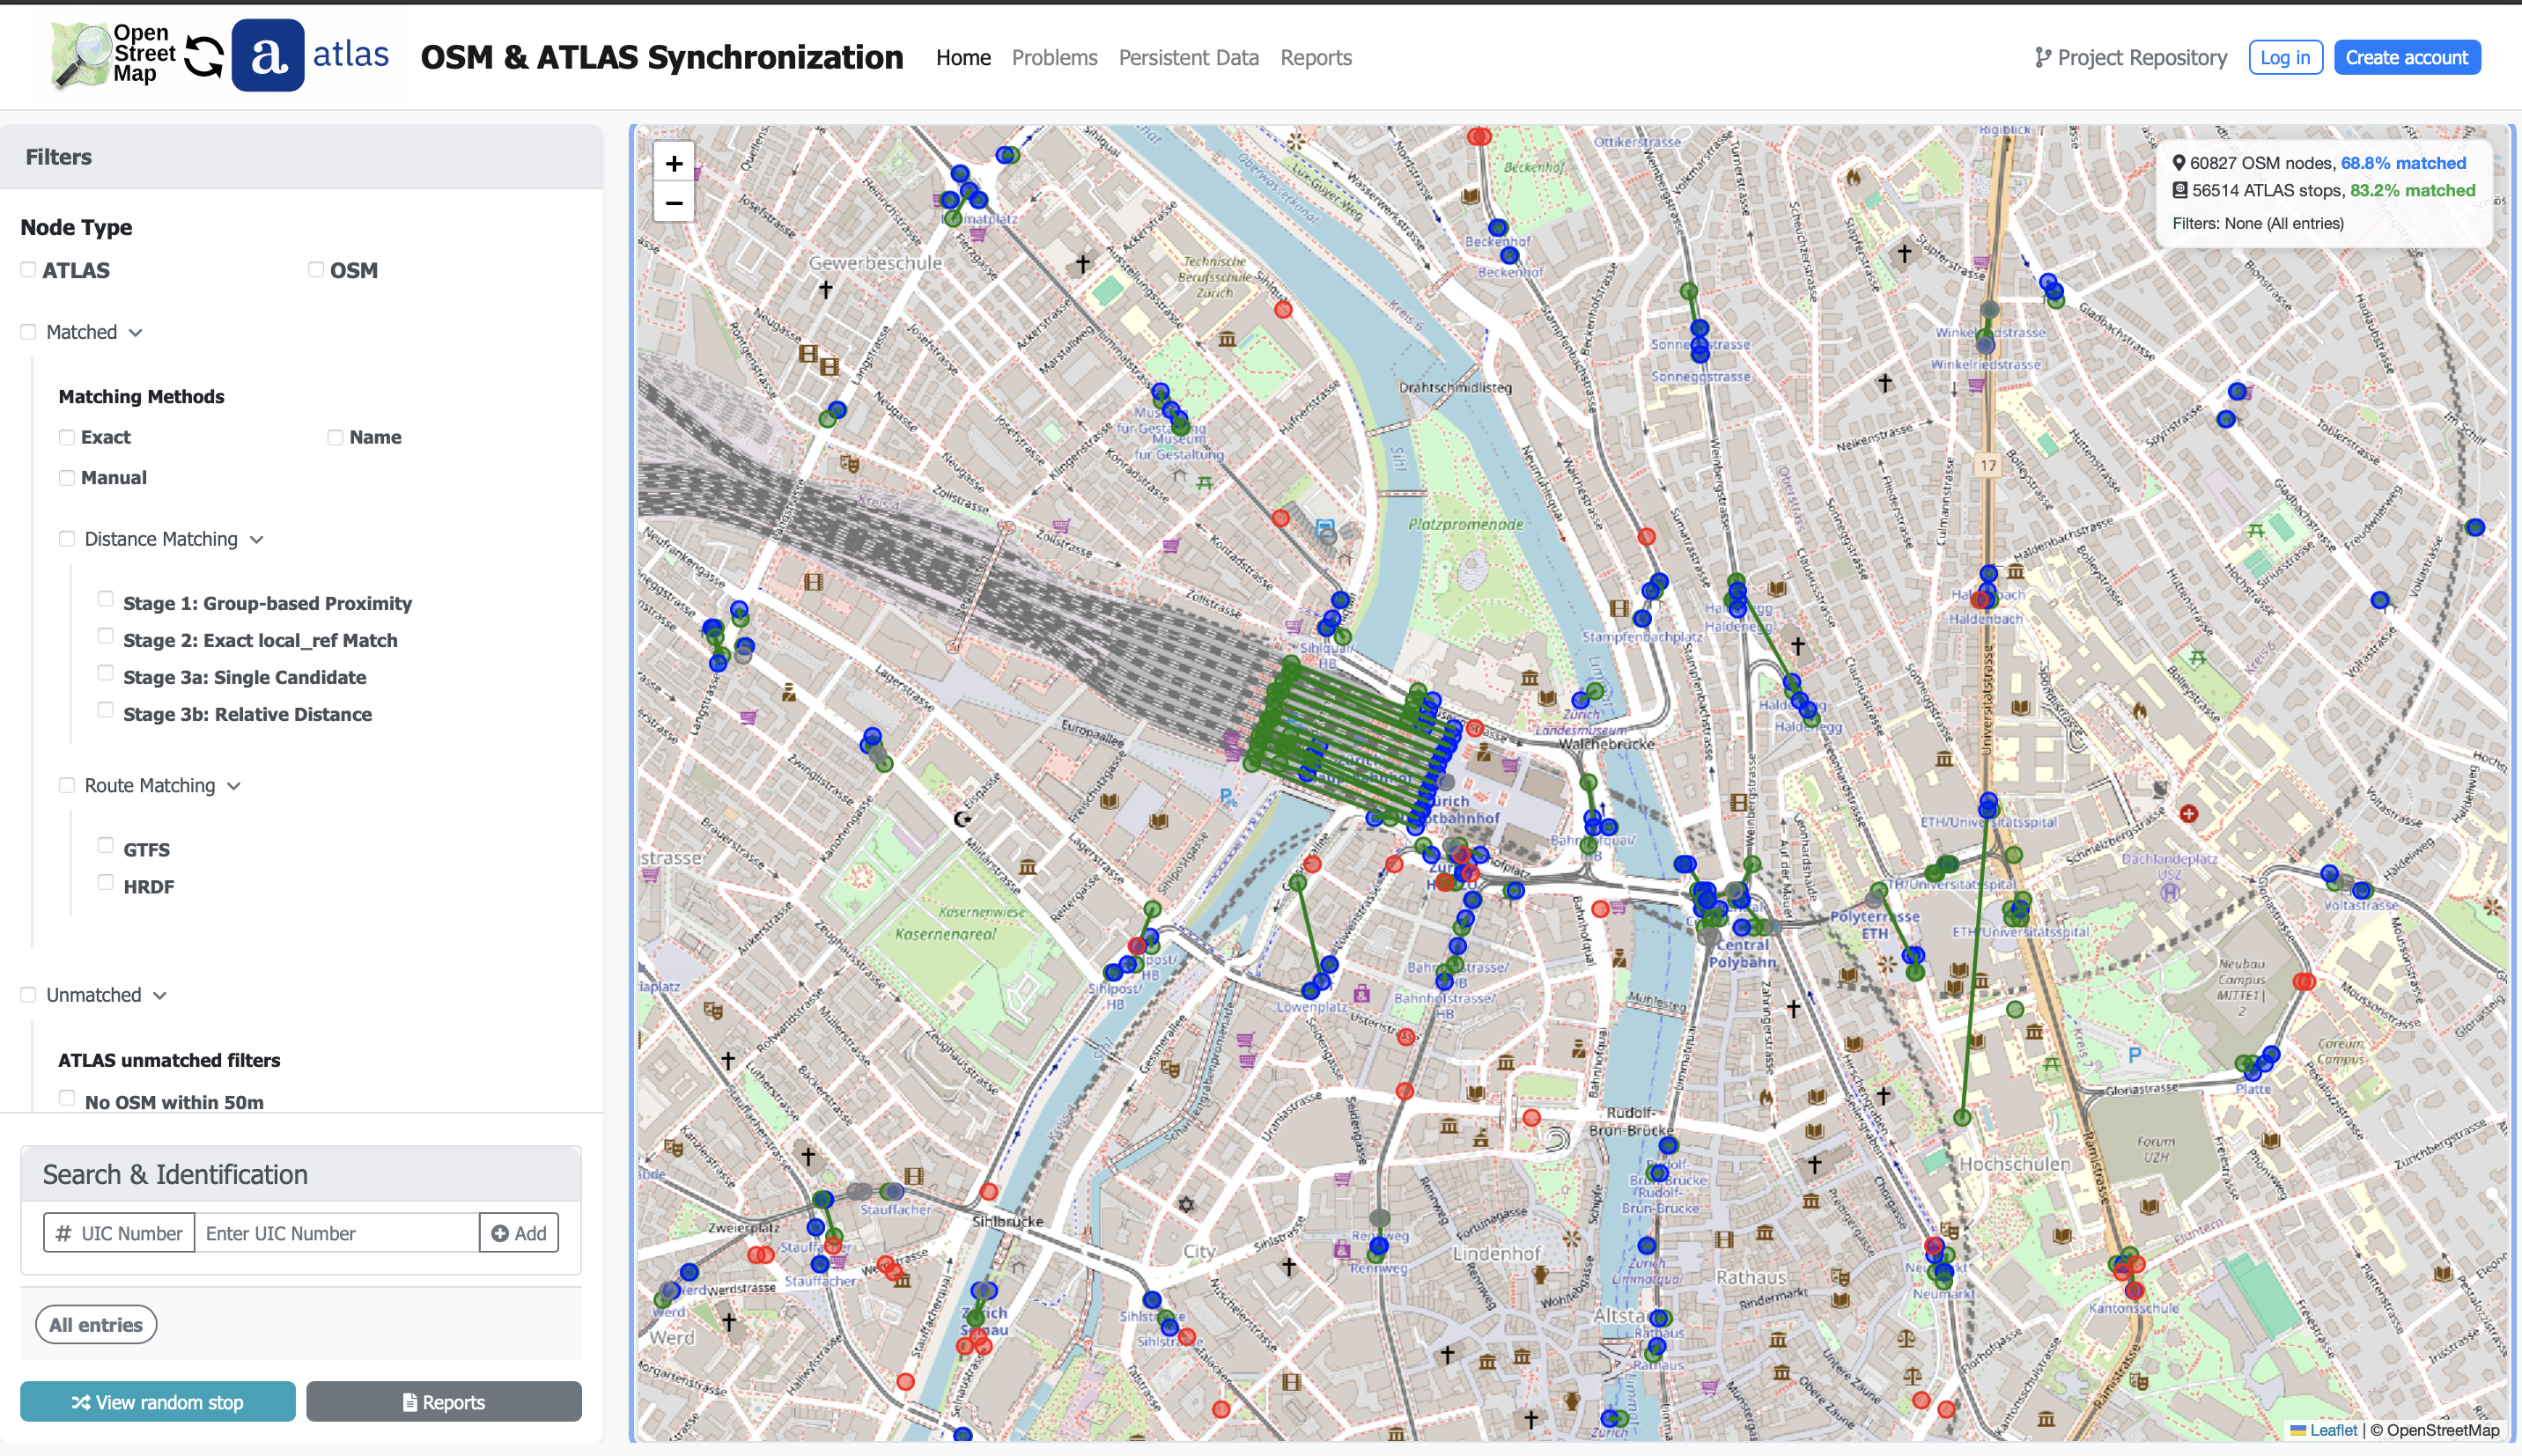
\includegraphics[width=0.95\textwidth]{../figures/chap9/main_page.png}
  \caption{Vue générale de la page d'accueil}
  \label{fig:frontend-index-main}
\end{figure}

\begin{figure}[h]
  \centering
  \includegraphics[width=0.95\textwidth]{../figures/chap9/atlas filter activ main page.png}
  \caption{Filtre ATLAS activé — ville de Zurich}
  \label{fig:frontend-index-filters}
\end{figure}

\section{Pages et navigation}

L'application comporte quatre vues principales :
\begin{itemize}
  \item \textbf{Carte (Index)} — exploration des arrêts, filtres riches, info-bulles, et un \emph{Top~N} des plus grandes distances. (Template: \texttt{templates/pages/index.html})
  \item \textbf{Problèmes} — tri, filtrage et résolution guidée des anomalies avec contexte cartographique local. (\texttt{templates/pages/problems.html})
  \item \textbf{Données persistantes} — revue et gestion des solutions/notes persistées entre imports. (\texttt{templates/pages/persistent\_data.html})
  \item \textbf{Rapports} — page dédiée de configuration et rendu PDF/CSV via backend (\texttt{templates/pages/reports.html}, cf. \S\ref{subsec:rapports}).
\end{itemize}

Chaque page est construite en HTML Jinja, stylisée par les feuilles CSS du dossier \texttt{static/css}, et animée par du JavaScript modulaire dans \texttt{static/js}.

\section{Carte interactive (Index)}

\subsection{Cycle de vie des requêtes}
La carte (Leaflet) initialise une vue par défaut et \textbf{anti-rebondit} les événements \texttt{moveend}/\texttt{zoomend} (\(\sim\)320~ms) avant de charger la nouvelle fenêtre d'affichage. Les requêtes en vol sont \textbf{annulées} lorsque l'utilisateur se déplace à nouveau, ce qui évite les rendus obsolètes. Les paramètres envoyés à l'API incluent la \textit{bbox} et les filtres actifs. Références côté serveur: \texttt{/api/data} and \texttt{/api/stop\_popup} (voir Chap.~8 pour la logique et la sérialisation).

\begin{itemize}
  \item \textbf{Seuils de zoom} — pas de marqueurs en dessous de \(z<13\); les \textit{polylignes} de liaison ne s'affichent qu'à partir de \(z\ge 14\).
  \item \textbf{Petits ensembles à faible zoom} — une \textit{sonde} plafonnée à \(\leq 250\) entrées permet d'afficher un petit ensemble même à bas zoom; sinon, une bannière invite à zoomer.
  \item \textbf{Milieu de zoom} — résultats plafonnés (\(\leq 500\)).
  \item \textbf{Fort zoom} — plafond levé: \emph{tous} les marqueurs de la fenêtre sont renvoyés.
\end{itemize}

\noindent
\textit{Capture d'écran} : bannière ``zoomez'' et apparitions des marqueurs.

\begin{figure}[h]
  \centering
  \includegraphics[width=0.9\textwidth]{../figures/chap9/zoom_in_to_see_all_stop_markers.png}
  \caption{Bannière politique de rendu selon le niveau de zoom}
  \label{fig:frontend-zoom-banner}
\end{figure}

\subsection{Rendu des marqueurs et des lignes}
Le rendu privilégie des cercles Canvas/SVG légers jusqu'au zoom \(z<18\). Au-delà, certaines icônes \textit{lettrees} (\texttt{D}, \texttt{P}, \texttt{S}) sont utilisées pour signaler \textit{duplicate}, \textit{platform}, \textit{station}. Les icônes DOM identiques sont \textbf{mises en cache} pour éviter les reconstructions inutiles.

Lorsque des marqueurs se superposent exactement, un \textbf{décalage circulaire} subtil est appliqué pour éviter l'occlusion. Les ajouts au calque sont \textbf{lotis} (\(\sim\)150–200 par lot) afin de préserver la réactivité du thread principal.

Les paires appariées (ATLAS–OSM) peuvent afficher une \textbf{ligne de liaison} (verte par défaut; violette pour un match manuel, en pointillés si non persistant) lorsque les deux extrémités sont visibles et que le zoom le permet.

% (figure déplacée vers la section Filtres)

\subsection{Info-bulles et chargement paresseux}
Le contenu des popups est rendu par un \textbf{moteur de gabarits côté client} (\texttt{PopupRenderer}). Un premier clic déclenche un appel à \texttt{/api/stop\_popup} qui renvoie des détails enrichis (noms, opérateurs, routes, notes). Les vues \textit{unifiées} permettent d'inspecter \textbf{toutes les correspondances} d'un nœud (ATLAS \emph{vs} OSM) sans recharger la page. Les popups sont déplaçables et conservent une \textit{ligne d'ancrage} lors des déplacements/zooms.

Pour les entrées non appariées, un bouton \texttt{Match to} apparaît dans l'info-bulle. La sélection d'une cible opposée (ATLAS \(\leftrightarrow\) OSM) déclenche la création d'un match manuel via \texttt{/api/manual\_match}. Cette action est cohérente avec le \textit{workflow} décrit au Chap.~8 (persistance optionnelle).

\begin{figure}[h]
  \centering
  \includegraphics[width=0.85\textwidth]{../figures/chap9/popups.png}
  \caption{Info-bulles}
  \label{fig:frontend-popups}
\end{figure}

\subsection{Panneau de filtres et recherche}
Le panneau de gauche agrège des filtres \textbf{par domaines fonctionnels} :
\begin{itemize}
  \item \textbf{Type de nœud} (ATLAS/OSM) et \textbf{Type d'arrêt} (\textit{Matched}, \textit{Unmatched}, \textit{Station}).
  \item \textbf{Méthodes d'appariement}: Exact, Name, Manual; \textbf{Distance Matching} (stages 1, 2, 3a, 3b); \textbf{Route Matching} (GTFS, HRDF).
  \item \textbf{Top N Distances} — surcouche légère pour inspecter rapidement les plus grandes distances.
  \item \textbf{Transports} (station, platform, stop\_position, ferry, aerialway, tram, etc.).
  \item \textbf{Opérateurs ATLAS} — \textit{dropdown} dédié avec recherche (chargé depuis \texttt{/api/operators}).
  \item \textbf{Filtres spéciaux} — afficher uniquement les \textit{duplicates} ATLAS.
\end{itemize}

La zone \textit{Active Filters} affiche des \textbf{"chips"} cliquables (ET/OU) pour retirer rapidement un critère. Un \textbf{sélecteur de type de recherche} (numéro UIC, SLOID ATLAS, OSM Node ID, Route ID) ajuste dynamiquement le champ de saisie et les actions associées. Un \textbf{résumé d'en-tête} interroge \texttt{/api/global\_stats} pour afficher des indicateurs utiles (ex.: pourcentage de nœuds appariés) synchronisés avec les filtres.

\begin{figure}[h]
  \centering
  \includegraphics[width=\textwidth]{../figures/chap9/filter_chips_index.png}
  \caption{Panneau de filtres avec \og chips \fg{} actifs}
  \label{fig:frontend-filters-chips}
\end{figure}

\begin{figure}[h]
  \centering
  \includegraphics[width=\textwidth]{../figures/chap9/stats box.png}
  \caption{Résumé d'en-tête avec statistiques globales. 3 filtres actifs}
  \label{fig:frontend-filters}
\end{figure}

\section{Outil Problèmes}

La page \textbf{Problèmes} combine : un panneau de filtres repliable (type d'anomalie, tri, opérateurs, priorité), une \textbf{carte de contexte} locale (\(\pm 0.02^\circ\)), et un \textbf{panneau de résolution} avec navigation par entrées. Les raccourcis clavier accélèrent la revue (\(\rightarrow\)/Espace: suivant, \(\leftarrow\): précédent, \(\uparrow\)/\(\downarrow\): défilement).

Les boutons d'action proposent des solutions pré-remplies (selon le type d'anomalie), la \textbf{persistance} des corrections, et l'édition de \textbf{notes} ATLAS/OSM. Le \textit{toggle} \texttt{Auto-Persist} permet de rendre persistantes toutes les nouvelles solutions/notes ; l'information est stockée pour être \textbf{réappliquée automatiquement} lors d'un prochain import (voir \S\,\emph{Persistance} et Chap.~8).

\begin{figure}[h]
  \centering
  \includegraphics[width=0.9\textwidth]{../figures/chap9/problems page.png}
  \caption{Page Problèmes — vue d'ensemble : filtres, carte de contexte et panneau de résolution}
  \label{fig:frontend-problems}
\end{figure}

\begin{figure}[h]
  \centering
  \begin{minipage}[b]{0.48\textwidth}
    \centering
    \includegraphics[width=\textwidth]{../figures/chap9/problems priority filter.png}
    \caption*{Filtre de priorité et tri.}
  \end{minipage}\hfill
  \begin{minipage}[b]{0.48\textwidth}
    \centering
    \includegraphics[width=\textwidth]{../figures/chap9/problems fiterchips and persistence options toggles.png}
    \caption*{Chips actifs et options de persistance.}
  \end{minipage}
  \caption{Contrôles de filtrage et options de persistance — Page Problèmes}
\end{figure}

\begin{figure}[h]
  \centering
  \begin{minipage}[b]{0.48\textwidth}
    \centering
    \includegraphics[width=\textwidth]{../figures/chap9/distance problem resolution actions.png}
    \caption*{Actions proposées : problèmes de distance.}
  \end{minipage}\hfill
  \begin{minipage}[b]{0.48\textwidth}
    \centering
    \includegraphics[width=\textwidth]{../figures/chap9/problem resolution actions attributes problem.png}
    \caption*{Actions proposées : problèmes d'attributs.}
  \end{minipage}
  \caption{Panneau de résolution — actions contextuelles selon le type d'anomalie}
\end{figure}

\section{Données persistantes}

La page \textbf{Données persistantes} distingue les \textit{persistantes} (appliquées après import) des \textit{non persistantes}. On peut filtrer par type (distance, unmatched, attributes, notes) et effectuer des actions massives (\textit{Make All Persistent}, suppression/vidage). Côté serveur, ces opérations appellent les endpoints dédiés décrits au Chap.~8.

\begin{figure}[h]
  \centering
  \includegraphics[width=0.9\textwidth]{../figures/chap9/non admin persisten data page.png}
  \caption{Données persistantes — pour utilisateurs non administrateurs}
  \label{fig:frontend-persistent}
\end{figure}

\section{Rapports et instantanés}
\label{subsec:rapports}

Une \textbf{page dédiée} (\texttt{/reports}) propose un formulaire de configuration pour générer des rapports (\textit{Top Matches}, \textit{Exact}, \textit{Name}, \textit{Duplicates}) en PDF ou CSV via l'endpoint \texttt{/api/generate\_report} (voir Chap.~8). Un \textbf{plafond de 20 téléchargements par IP et par jour} est appliqué côté serveur (limiteur global avec règle spécifique à l'endpoint) pour garantir un usage équitable. Un \textbf{instantané de carte} (\texttt{map\_snapshot.html}) peut afficher un groupe UIC/Opérateur avec marqueurs et liaisons, utile pour des annexes ou l'intégration dans le mémoire.

\begin{figure}[h]
  \centering
  \includegraphics[width=0.9\textwidth]{../figures/chap9/download reports page.png}
  \caption{Page Rapports — génération (PDF/CSV) et limite quotidienne}
  \label{fig:frontend-report}
\end{figure}

\section{Liaison avec le backend (rappel Chap. 8)}

La cohérence et la réactivité de l'interface reposent sur:
\begin{itemize}
  \item \texttt{/api/data} — charge utile \textbf{minimale} pour la navigation (coordonnées, types, distance, identifiants).
  \item \texttt{/api/stop\_popup} — \textbf{détails} à la demande pour les info-bulles.
  \item \texttt{/api/top\_matches}, \texttt{/api/global\_stats} — \textbf{synthèses} parallèles non bloquantes.
  \item \texttt{/api/manual\_match}, \texttt{/api/save\_solution}, \texttt{/api/make\_solution\_persistent}, \texttt{/api/save\_note} — actions \textbf{créatrices} assorties d'une option de persistance.
\end{itemize}

Ces endpoints, leurs limites de débit et la sérialisation \texttt{format\_stop\_data()} sont détaillés au Chapitre~8.

\section*{Conclusion}

Le frontend associe une carte \textbf{fluide} (anti-rebond, annulation, seuils de zoom) à des \textbf{filtres expressifs} et à des info-bulles \textbf{paresseuses} pour conserver des charges utiles petites. L'outil Problèmes structure le travail de gestion des données et  persistance des données rendant les corrections \textbf{durables} entre imports. La génération de rapports complète l'ensemble en offrant des exports soignés.

% !TeX spellcheck = fr_FR
\chapter{Chapitre 10: Système d'authentification sécurisé}\label{chap:auth}

\section{Objectifs}
Nous avons conçu et mis en œuvre un système d'authentification complet, aligné sur les bonnes pratiques actuelles.

\section{Aperçu de l'architecture}
L'application utilise un schéma d'authentification dédié lié à une base de données MySQL distincte (\texttt{auth\_db}). Comme on a vu, les donnée principales de l'application demeurent dans \texttt{stops\_db}. Cette séparation réduit le rayon d'impact et garantit entre d'autres choses que la réimportation des données de transport public ne touche jamais les identifiants des utilisateurs.

\subsection{Composants}
\begin{itemize}
  \item \textbf{Stockage des mots de passe} : Argon2id (argon2-cffi), à forte consommation mémoire, salé, avec des paramètres spécifiques à chaque hachage.
  \item \textbf{Sessions} : Flask-Login avec cookies sécurisés (HttpOnly, SameSite=Lax ; indicateur Secure en production).
  \item \textbf{CSRF} : Protection CSRF de Flask-WTF pour tous les formulaires POST et les points de terminaison concernés.
  \item \textbf{Limitation de débit} : Les routes de connexion et d'inscription sont limitées (Flask-Limiter) afin d'atténuer la force brute.
  \item \textbf{Sécurité du transport} : Flask-Talisman fournit les en-têtes de sécurité ; application stricte de HTTPS.
  \item \textbf{2FA} : TOTP (compatible Google Authenticator) avec activation par QR code et codes de secours à usage unique. \textbf{Le secret TOTP est chiffré au repos} (Fernet) ; les codes de secours sont hachés (Argon2).
  \item \textbf{Verrouillage de compte} : Verrouillage progressif après des échecs répétés, avec temporisation exponentielle.
  \item \textbf{Vérification d'email} : Liens signés (validité 48 h) envoyés à l'inscription et lors d'une connexion non vérifiée. La vérification est \emph{optionnelle par défaut}.
  \item \textbf{CAPTCHA} : Cloudflare Turnstile sur \texttt{/auth/register} et \texttt{/auth/login}.
  \item \textbf{Journalisation d'audit} : enregistrement des événements d'authentification dans \texttt{auth\_db.auth\_events} et émission simultanée de logs JSON sur \texttt{stdout}

\section{Modèle de données (auth\_db)}
La table \texttt{users} stocke les comptes utilisateurs avec les champs suivants :

\noindent\begin{tabular}{@{}p{0.40\linewidth}p{0.60\linewidth}@{}}
\textbf{Identité} & \texttt{email} (unique) \\
\textbf{Authentification} & \texttt{password\_hash} (Argon2id) \\
\textbf{Rôles} & \texttt{is\_admin} \\
\textbf{Vérification d'email} & \texttt{is\_email\_verified}, \texttt{email\_verified\_at}, \texttt{last\_verification\_sent\_at} \\
\textbf{2FA} & \texttt{is\_totp\_enabled}, \texttt{totp\_secret} \\
\textbf{Codes de secours} & JSON de hachés Argon2 \\
\textbf{Hygiène de compte} & \texttt{created\_at}, \texttt{updated\_at}, \texttt{last\_login\_at} \\
\textbf{Verrouillage} & \texttt{failed\_login\_attempts}, \texttt{locked\_until} \\
\end{tabular}


\subsection*{Journalisation d'audit (\texttt{auth\_events})}
\noindent Une table \texttt{auth\_events} (même schéma \texttt{auth\_db}) consigne les événements de sécurité :

\noindent\begin{tabular}{@{}p{0.40\linewidth}p{0.60\linewidth}@{}}
\textbf{Type d'événement} & \texttt{event\_type} (\textit{registration}, \textit{login\_success}, \textit{login\_failure}, \textit{account\_locked}, \textit{2fa\_success}, \textit{2fa\_failure}, \textit{2fa\_enabled}, \textit{2fa\_disabled}, \textit{email\_verified}) \\
\textbf{Utilisateur} & \texttt{user\_id} (nullable), \texttt{email\_attempted} (pour les échecs) \\
\textbf{Contexte} & \texttt{ip\_address}, \texttt{user\_agent} \\
\textbf{Détails} & \texttt{metadata\_json} \\
\textbf{Horodatage} & \texttt{occurred\_at} (UTC) \\
\end{tabular}

\begin{codebox}[language=Python]{Modèle minimal (extrait)}
class AuthEvent(db.Model):
    __bind_key__ = 'auth'
    __tablename__ = 'auth_events'
    id = db.Column(db.Integer, primary_key=True)
    user_id = db.Column(db.Integer, db.ForeignKey('users.id'), index=True)
    email_attempted = db.Column(db.String(255), index=True)
    event_type = db.Column(db.String(50), nullable=False, index=True)
    ip_address = db.Column(db.String(45))
    user_agent = db.Column(db.Text)
    metadata_json = db.Column(db.Text)
    occurred_at = db.Column(db.DateTime, default=utcnow, index=True)
\end{codebox}

\noindent Les mêmes événements sont émis au format JSON sur la sortie standard du service pour une collecte centralisée.
\subsection{Parcours utilisateur et impact sur les données}
Cette sous-section illustre, étape par étape, comment les actions de l'utilisateur se traduisent dans le schéma \texttt{auth\_db}.

\paragraph{Accès aux écrans d'authentification}
\begin{figure}[H]
  \centering
  \includegraphics[width=0.85\textwidth]{../figures/chap10/auth1.png}
  \caption{Bouton \og Créer un compte \fg{} visible dans l'interface.}
\end{figure}

\paragraph{Inscription}
Un utilisateur fournit un email et un mot de passe ; le serveur hache le mot de passe avec Argon2id et crée la ligne dans \texttt{users}.

\begin{codebox}[language=Python]{Hachage du mot de passe (inscription)}
from argon2 import PasswordHasher
ph = PasswordHasher()
password_hash = ph.hash(plain_password)
\end{codebox}

\begin{figure}[H]
  \centering
  \includegraphics[width=0.85\textwidth]{../figures/chap10/create_account.png}
  \caption{Formulaire d'inscription (email, mot de passe).}
\end{figure}

\begin{figure}[H]
  \centering
  \includegraphics[width=0.85\textwidth]{../figures/chap10/auth_db1.png}
  \caption{\texttt{auth\_db.users}: \texttt{email} et \texttt{password\_hash} après inscription.}
\end{figure}

\paragraph{Vérification d'email}
À l'inscription, un lien de vérification signé (valide 48 h) est envoyé. Lorsqu'un utilisateur non vérifié se connecte avec succès, l'application \textbf{autorise la connexion} et renvoie un nouvel email de vérification accompagné d'un avertissement UI. Des routes dédiées existent pour \textit{vérifier} (\texttt{/auth/verify-email/<token>}) et \textit{renvoyer} (\texttt{/auth/resend-verification}) le lien. Cette vérification peut être rendue obligatoire côté produit si nécessaire.

\begin{figure}[H]
  \centering
  \fbox{\parbox{0.8\textwidth}{\centering Placeholder visuel pour la capture de la vérification d'email.\\ Lien signé, expiration 48~h, renouvelable.}}
  \caption{Processus de vérification d'email (espace réservé).}
\end{figure}

\begin{codebox}[language=Python]{Jeton de vérification d'email (extrait)}
from itsdangerous import URLSafeTimedSerializer
s = URLSafeTimedSerializer(SECRET_KEY, salt="email-verification")
token = s.dumps({"uid": user_id})
# Plus tard:  uid = int(s.loads(token, max_age=60*60*48)["uid"])  # 48 h
\end{codebox}

\noindent\textbf{Délivrance des emails (Amazon SES).} Les emails de vérification sont rendus côté serveur puis envoyés via Amazon Simple Email Service (SES) grâce au SDK \texttt{boto3}. La fonction \texttt{send\_email(...)} centralise l'envoi dans \texttt{backend/services/email.py} et lit sa configuration via variables d'environnement :
\begin{itemize}
  \item \texttt{AWS\_REGION} (p.~ex. \texttt{eu-west-1})
  \item \texttt{SES\_FROM\_EMAIL} (identité SES vérifiée)
  \item \texttt{SES\_CONFIGURATION\_SET} (optionnel)
\end{itemize}
Le flux d'envoi est déclenché depuis \texttt{backend/blueprints/auth.py} : l'application génère le lien signé, rend les gabarits d'email (HTML et texte) dans \texttt{templates/emails/}, puis appelle \texttt{send\_email(...)}. Les erreurs d'envoi sont journalisées mais n'interrompent pas le parcours utilisateur, afin d'éviter toute fuite d'information et de préserver l'ergonomie.

\begin{figure}[H]
  \centering
  \includegraphics[width=0.85\textwidth]{../figures/chap10/auth_db2.png}
  \caption{\texttt{auth\_db.users}: \texttt{is\_admin}, \texttt{is\_email\_verified}, \texttt{last\_verification\_sent\_at}, \texttt{is\_totp\_enabled}.}
\end{figure}

\paragraph{Connexion}
L'utilisateur s'authentifie sur la page de connexion ; en cas de succès, l'application met à jour l'historique de connexion et applique le verrouillage en cas d'échecs répétés.

\begin{figure}[H]
  \centering
  \includegraphics[width=0.85\textwidth]{../figures/chap10/login_page.png}
  \caption{Page de connexion. Les limites de débit et le CAPTCHA (Turnstile) freinent les robots (voir Chap.~\ref{chap:security}).}
\end{figure}

\begin{figure}[H]
  \centering
  \includegraphics[width=0.85\textwidth]{../figures/chap10/login_succesful.png}
  \caption{Connexion réussie: alertes UI sur l'email non vérifié et la 2FA non activée.}
\end{figure}

\begin{figure}[H]
  \centering
  \includegraphics[width=0.85\textwidth]{../figures/chap10/auth_db4.png}
  \caption{\texttt{auth\_db.users}: \texttt{last\_login\_at}, \texttt{failed\_login\_attempts}, \texttt{locked\_until}.}
\end{figure}

\paragraph{2FA}
Lorsqu'un utilisateur active la 2FA, le serveur génère un secret Base32 aléatoire et affiche un QR code contenant une URI \textit{otpauth} standard. \textbf{Ce secret est chiffré au repos} (\texttt{cryptography.Fernet}) avec une clé d'application fournie par variable d'environnement, puis stocké dans \texttt{auth\_db.users.totp\_secret}. L'utilisateur vérifie le premier code à 6 chiffres pour activer la 2FA. Le serveur génère 10 codes de secours à usage unique et n'en stocke que les versions hachées avec Argon2. À la connexion, si la 2FA est active, l'utilisateur doit fournir un TOTP valide ou un code de secours non utilisé.

\begin{figure}[H]
  \centering
  \includegraphics[width=0.85\textwidth]{../figures/chap10/enable_up2fa.png}
  \caption{Activation 2FA avec QR \textit{otpauth://} et secret Base32. QR et secret encodent la même information.}
\end{figure}

\begin{codebox}[language=Python]{Validation TOTP (connexion avec 2FA)}
import pyotp
secret = user.get_totp_secret()  # déchiffre à la volée si chiffré
is_valid = pyotp.TOTP(secret).verify(code, valid_window=1)
\end{codebox}

\begin{figure}[H]
  \centering
  \includegraphics[width=0.85\textwidth]{../figures/chap10/backupcodes.png}
  \caption{Codes de secours: affichés une seule fois à l'activation. Stockage côté serveur: hachés Argon2 dans un JSON.}
\end{figure}

\begin{figure}[H]
  \centering
  \includegraphics[width=0.85\textwidth]{../figures/chap10/enter2FA.png}
  \caption{Étape de connexion avec saisie du code 2FA (ou d'un code de secours).}
\end{figure}

\begin{figure}[H]
  \centering
  \includegraphics[width=0.85\textwidth]{../figures/chap10/auth_db3.png}
  \caption{\texttt{auth\_db.users}: \texttt{totp\_secret} (chiffré), \texttt{backup\_codes\_json} (haché), \texttt{created\_at}, \texttt{updated\_at}.}
\end{figure}

\section{Sécurité opérationnelle (en pratique)}
\noindent Cette section résume les mesures concrètes d'exploitation sécurisée et l'intention derrière chacune.

\begin{itemize}
  \item \textbf{Secrets et configuration} : Les clés d'application (\texttt{SECRET\_KEY}), URL de base (\texttt{AUTH\_DATABASE\_URI}) et HTTPS sont fournis par variables d'environnement (Docker Compose). Ils ne sont jamais versionnés.
  \item \textbf{Mots de passe et codes} : Rien n'est stocké en clair. Les mots de passe sont hachés (Argon2id) ; les codes de secours sont également hachés.
  \item \textbf{Moindre privilège} : \texttt{auth\_db} utilise des comptes dédiés avec des droits minimaux ; chaque service n'accède qu'au strict nécessaire.
  \item \textbf{Protection contre les attaques} : Limitation de débit, verrouillage progressif et CAPTCHA atténuent la force brute et le bourrage d'identifiants.
  \item \textbf{En-têtes et CSP} : Talisman applique les en-têtes de sécurité et une politique CSP. Cette CSP peut être durcie en réduisant l'usage de CDN.
  \item \textbf{Traçabilité} : Les événements d'authentification sont consignés dans \texttt{auth\_events} et envoyés en logs JSON pour la supervision.
\end{itemize}




% !TeX spellcheck = fr_FR
\chapter{Chapitre 11: Évaluation de la sécurité de l'application}\label{chap:security}

\noindent Ce chapitre complète le \textbf{Chap.~\ref{chap:auth}} en évaluant les défenses mises en place, en illustrant les scénarios d'attaque plausibles et en discutant des améliorations futures. L'objectif est de comprendre comment et pourquoi les contrôles bloquent les attaques.

\section{Périmètre et surface d'attaque}
\noindent Pour rendre la lecture concrète, nous partons d'une \emph{carte des routes} — celles que l'utilisateur peut réellement atteindre. Nous indiquons les garde-fous (authentification, limites de débit) directement à côté de chaque groupe.

\paragraph{Pages (UI)} \texttt{/}, \texttt{/map\_snapshot}, \texttt{/problems}, \texttt{/persistent\_data}, \texttt{/reports} — vues HTML publiques qui appellent l'API ci-dessous.

\paragraph{Authentification} (limitées par IP)
\begin{itemize}
  \item \texttt{/auth/register} \textit{GET,POST} — \textbf{5/min}; CAPTCHA Turnstile
  \item \texttt{/auth/login} \textit{GET,POST} — \textbf{10/min}; CAPTCHA + verrouillage progressif par compte
  \item \texttt{/auth/2fa} \textit{GET,POST} — \textbf{15/min}
  \item \texttt{/auth/logout} \textit{POST} — \textbf{auth requis}
  \item \texttt{/auth/enable\_2fa} \textit{GET,POST} — \textbf{auth requis}
  \item \texttt{/auth/disable\_2fa} \textit{POST} — \textbf{auth requis}
  \item \texttt{/auth/verify-email/<token>} \textit{GET} — \textbf{30/h}
  \item \texttt{/auth/resend-verification} \textit{GET,POST} — \textbf{5/min} (réponse neutre)
  \item \texttt{/auth/status} \textit{GET}
\end{itemize}

\paragraph{Données} (lecture cartographique)
\begin{itemize}
  \item \texttt{/api/data} \textit{GET} — \textbf{30/min}; filtrage \emph{SARGable} sur la fenêtre \texttt{bbox}, pagination
  \item \texttt{/api/stop\_popup} \textit{GET} — \textbf{120/min}; jointures ciblées, sérialisation compacte
  \item \texttt{/api/route\_stops} \textit{GET} — \textbf{60/min}; requête optimisée + fallback de normalisation
  \item \texttt{/api/operators} \textit{GET} — \textbf{60/min}; \texttt{SELECT DISTINCT} indexé
\end{itemize}

\paragraph{Recherche}
\begin{itemize}
  \item \texttt{/api/search} \textit{GET} — \textbf{60/min}; colonnes réduites via \texttt{optimize\_query\_for\_endpoint}
  \item \texttt{/api/top\_matches} \textit{GET} — \textbf{60/min}; tri sur colonne indexée \texttt{distance\_m}
  \item \texttt{/api/random\_stop} \textit{GET} — \textbf{30/min}; \emph{sampling} par plages d'ID (pas de \texttt{ORDER BY RAND()})
  \item \texttt{/api/stop\_by\_id} \textit{GET} — \textbf{60/min}
  \item \texttt{/api/manual\_match} \textit{POST} — \textbf{30/min}; enregistre un appariement manuel
\end{itemize}

\paragraph{Statistiques et rapports}
\begin{itemize}
  \item \texttt{/api/global\_stats} \textit{GET} — \textbf{30/min}; cache LRU en mémoire
  \item \texttt{/api/generate\_report} \textit{GET} — \textbf{auth requis}, \textbf{20/jour}; génération PDF/CSV côté serveur
\end{itemize}

\paragraph{Problèmes et persistance}
\begin{itemize}
  \item \texttt{/api/problems}, \texttt{/api/problems/stats} \textit{GET} — \textbf{120/min}
  \item \texttt{/api/save\_solution}, \texttt{/api/make\_solution\_persistent} \textit{POST} — \textbf{30/min}, \textbf{auth requis}
  \item \texttt{/api/save\_note/atlas}, \texttt{/api/save\_note/osm}, \texttt{/api/make\_note\_persistent/<type>} \textit{POST} — \textbf{60/min}, \textbf{auth requis}
  \item \texttt{/api/check\_persistent\_solution}, \texttt{/api/check\_persistent\_note/...} \textit{GET} — \textbf{120/min}
  \item \texttt{/api/persistent\_data}, \texttt{/api/non\_persistent\_data} \textit{GET} — \textbf{60/min}, \textbf{auth requis}
  \item \texttt{/api/persistent\_data/<id>} \textit{DELETE} — \textbf{30/min}, \textbf{auth+admin}
  \item \texttt{/api/make\_non\_persistent/<id>}, \texttt{/api/clear\_all\_persistent}, \texttt{/api/clear\_all\_non\_persistent}, \texttt{/api/make\_all\_persistent} \textit{POST} — \textbf{10/h}, \textbf{auth requis} (admin si destructif)
\end{itemize}

\noindent \textbf{Important}. Les opérations \emph{destructives} sur les données persistantes (comme \texttt{DELETE /api/persistent\_data/<id>}) sont réservées aux \textbf{administrateurs}. Un utilisateur non admin ne peut ni supprimer ni vider ces jeux de données.

\section{Contrôles en place}

\subsection*{Mots de passe et stockage}
\noindent Les mots de passe sont hachés avec Argon2id\citeref{ref:argon2_docs} via \texttt{argon2-cffi}, avec paramètres adaptés à la mémoire. Vérification sûre:
\begin{codebox}[language=Python]{Vérifier un mot de passe}
from argon2 import PasswordHasher
ph = PasswordHasher()
ph.verify(user.password_hash, candidate)
\end{codebox}

\subsection*{Sessions et cookies}
\noindent Cookies \texttt{HttpOnly}, \texttt{SameSite=Lax} et \texttt{Secure} activable par variable d'environnement (en production : à forcer). Durée \og remember \fg{} de 14~jours.
\begin{codebox}[language=Python]{Paramètres de session (extrait)}
app.config['SESSION_COOKIE_HTTPONLY'] = True
app.config['SESSION_COOKIE_SAMESITE'] = 'Lax'
app.config['SESSION_COOKIE_SECURE'] = os.getenv('SESSION_COOKIE_SECURE','false').lower()=='true'
\end{codebox}

\subsection*{CSRF}
\noindent \textbf{Qu'est-ce que le CSRF ?} Une page malveillante pourrait faire envoyer à votre navigateur une requête \texttt{POST} à notre site en utilisant votre cookie de session, sans votre intention.

\noindent \textbf{Comment on s'en protège}. Les formulaires sensibles (inscription, connexion, 2FA, etc.) incluent un \textbf{jeton CSRF} caché généré par Flask-WTF. À chaque soumission, le serveur vérifie que le jeton du formulaire correspond à celui stocké côté session. Sans ce jeton, la requête est refusée.

\noindent \textbf{Qu'est exempté}. Les endpoints \textbf{lecture seule} JSON (\texttt{GET}) restent exemptés. Tout endpoint qui \textbf{modifie} de l'état via cookies de session doit exiger un jeton CSRF.

\noindent \texttt{SameSite=Lax} aide mais ne suffit pas: le jeton CSRF est la garantie principale contre l'exécution non intentionnelle de requêtes authentifiées.

\subsection*{CAPTCHA Turnstile}
\noindent Un CAPTCHA Cloudflare Turnstile\citeref{ref:cloudflare_turnstile} protège l'inscription et la connexion.
\begin{codebox}[language=Python]{Vérifier le CAPTCHA (simplifié)}
secret = os.getenv('TURNSTILE_SECRET_KEY','')
if not secret: return True  # dev
resp = requests.post('https://.../siteverify', data={...})
ok = bool(resp.json().get('success'))
\end{codebox}

\subsection*{Durcissement du conteneur}
\noindent \textbf{Principe du moindre privilège}. Le service \texttt{app} s'exécute désormais en \textbf{utilisateur non-root} (\texttt{USER app}) avec des \textbf{permissions minimales} dans \texttt{/app}. Seuls \texttt{/app/data} et \texttt{/app/.cache} sont inscriptibles; le reste du code est en lecture seule. En cas d'exécution de code arbitraire (RCE), l'impact est réduit par l'absence de droits \texttt{root}.

\noindent \textbf{Volumes et UID/GID}. Pour éviter des problèmes d'écriture sur le volume monté \texttt{.:/app}, l'UID/GID du compte \texttt{app} peut être aligné sur l'hôte via des \textit{build args} \texttt{APP\_UID}/\texttt{APP\_GID} (voir Chap.~\ref{chap:deploiement}).

\subsection*{Limitation de débit et verrouillage}
\noindent \textbf{Idée générale}. Nous combinons deux couches:
\begin{itemize}
  \item \textbf{Limites par route} (Flask-Limiter) — plafonds \og X par minute/heure/jour \fg{} appliqués par défaut \textbf{par IP}.
  \item \textbf{Verrouillage par compte} — après plusieurs mots de passe erronés, le compte est temporairement bloqué (délai croissant) pour ralentir les attaques.
\end{itemize}

\noindent \textbf{Comment les limites fonctionnent}. Chaque route a un \emph{quota} (ex.: \texttt{10/min}). À dépassement, le serveur répond \texttt{429 Too Many Requests}. Le plafonnement est appliqué \textbf{par IP}. En complément, un \textbf{verrouillage par compte} après plusieurs échecs empêche de contourner la seule limite IP.

\noindent \textbf{Caveat proxies}. Si l'application est derrière un proxy (NGINX/Cloudflare), il faut \textbf{configurer les proxys de confiance} pour lire correctement \texttt{X-Forwarded-For}. Sans cela, la limitation \og par IP \fg{} peut devenir inefficace ou injuste, car toutes les requêtes semblent provenir d'une même IP.
\begin{codebox}[language=Python]{Limites de débit par route}
@limiter.limit("5/minute")   # /auth/register
@limiter.limit("10/minute")  # /auth/login
@limiter.limit("15/minute")  # /auth/2fa
@limiter.limit("30/hour")    # /auth/verify-email/<token>
@limiter.limit("30/minute")  # /api/data
@limiter.limit("120/minute") # /api/stop_popup
@limiter.limit("60/minute")  # /api/search, /api/top_matches, /api/route_stops, /api/operators
@limiter.limit("30/minute")  # /api/random_stop, /api/manual_match
@limiter.limit("30/minute")  # /api/global_stats (avec cache LRU)
@login_required; @limiter.limit("20/day")  # /api/generate_report
\end{codebox}

\begin{codebox}[language=Python]{Verrouillage exponentiel (extrait)}
if not user.verify_password(password):
    user.failed_login_attempts += 1
    if user.failed_login_attempts >= 5:
        lock_minutes = min(60, 2 * user.failed_login_attempts + 5)
        user.locked_until = utcnow() + timedelta(minutes=lock_minutes)
\end{codebox}

\subsection*{2FA TOTP et codes de secours}
\noindent TOTP standard (30~s)\citeref{ref:totp_rfc} via \texttt{pyotp}. \textbf{Le secret TOTP est chiffré au repos} (Fernet)\citeref{ref:fernet_docs} et déchiffré à la volée à l'usage; les codes de secours sont \textbf{hachés} (Argon2) et \textbf{consommés} à l'usage.
\begin{codebox}[language=Python]{Vérifier TOTP ou code de secours}
secret = user.get_totp_secret()  # déchiffre si nécessaire
totp_ok = pyotp.TOTP(secret).verify(token, valid_window=1)
backup_ok = user.verify_and_consume_backup_code(token)
\end{codebox}

\subsection*{Journalisation d'audit}
\noindent Chaque tentative ou succès d'action sensible est consignée dans \texttt{auth\_db.auth\_events} et émise en JSON dans les logs:\
\begin{itemize}
  \item \textbf{Événements} : inscription, connexion (succès/échec), verrouillage, 2FA (succès/échec), activation/désactivation 2FA, email vérifié, logout.
  \item \textbf{Contexte} : IP (\texttt{X-Forwarded-For} prioritaire), \texttt{User-Agent}, email tenté (si échec), métadonnées.
  \item \textbf{Exploitation} : requêtes SQL côté \texttt{auth\_db} ou filtrage des logs \texttt{docker compose logs}.
\end{itemize}

\begin{codebox}[language=SQL]{Exemples de requêtes}
-- Connexions échouées pour un email sur 24 h
SELECT occurred_at, ip_address, metadata_json
FROM auth_events
WHERE event_type = 'login_failure'
  AND email_attempted = 'user@example.com'
  AND occurred_at > NOW() - INTERVAL 1 DAY
ORDER BY occurred_at DESC;
\end{codebox}

\begin{codebox}[language=bash]{Filtrer les événements dans les logs du conteneur}
docker compose logs -f app | grep 'auth_event' | cat
\end{codebox}

\section{Scénarios d'attaque et déroulé}

\subsection*{A1 — Bourrage d'identifiants / force brute}
\textbf{Attaque}. Un robot tente des listes \og email+mot de passe \fg{}.

\textbf{Côté serveur}. La route \texttt{/auth/login} est plafonnée à 10/min par IP; les échecs incrémentent un compteur par compte. Après 5 échecs: verrouillage progressif (5, 7, 9, ... minutes jusqu'à 60 min max). Cookies non délivrés tant que la session n'est pas authentifiée.

\textbf{Résultat}. Les rafales sont ralenties par IP (limiteur) et par compte (verrouillage), ce qui rend l'attaque coûteuse et lente. Des détails supplémentaires de calibrage sont discutés ci-dessous.

 

 

\subsection*{A2 — Contournement 2FA}
\textbf{Attaque}. L'attaquant dérobe un mot de passe (hameçonnage) et tente de se connecter sans 2FA.

\textbf{Côté serveur}. Si \texttt{is\_totp\_enabled=true}, une étape 2FA obligatoire s'intercale. Un TOTP valide (\textpm 30~s) ou un code de secours non consommé est requis.

\textbf{Résultat}. Sans le second facteur (ou un code de secours), l'intrusion échoue. Les codes de secours étant \textbf{hachés} et \textbf{consommés}, leur ré-utilisation est impossible.

 

 

\paragraph{Note}. Le secret TOTP est \textbf{chiffré au repos} dans \texttt{auth\_db} (Fernet), puis déchiffré à la volée pour la vérification. Les codes de secours restent hachés (Argon2) et sont consommés à l'usage.

\subsection*{A3 — Énumération d'email}
\textbf{Attaque}. Tester si un email existe via les messages d'erreur.

\textbf{Côté serveur}. \texttt{/auth/login} répond \og Invalid credentials \fg{} dans tous les cas; \texttt{/auth/resend-verification} répond identiquement qu'un compte existe ou non. \texttt{/auth/register} adopte désormais une \textbf{réponse neutre} : que l'email existe ou non, l'utilisateur est redirigé vers l'avis de vérification; si un compte non vérifié existe, un email de vérification est renvoyé en arrière-plan. Aucune information n'est divulguée sur l'existence du compte.

\textbf{Résultat}. L'énumération est évitée sur login/resend, mais possible sur register. Voir \S~\ref{sec:improve} pour uniformiser les messages.

 

\subsection*{A4 — Abus de liens signés (vérification d'email)}
\textbf{Attaques visées}.
\begin{itemize}
  \item \textbf{Rejeu} d'un vieux lien après vérification ou expiration.
  \item \textbf{Bruteforce} du jeton signé.
  \item \textbf{Inondation} d'envois de mails de vérification.
\end{itemize}

\textbf{Mesures côté serveur}.
\begin{itemize}
  \item Jetons \texttt{itsdangerous} avec \textbf{sel dédiée} et \textbf{expiration 48~h} ; taille et entropie suffisantes pour rendre le bruteforce irréaliste.
  \item Vérification idempotente: si l'email est déjà vérifié, le jeton est ignoré proprement.
  \item Plafonds: \texttt{/auth/verify-email/...} à \textbf{30/h} et \texttt{/auth/resend-verification} à \textbf{5/min}; côté application, \textbf{1 email/min par compte}.
  \item Journalisation d'audit des vérifications et des renvois pour repérer des abus.
\end{itemize}

\textbf{Effet}. Les relectures expirent rapidement ; les tentatives massives et le spam sont freinés par les limites.

 

\subsection*{A5 — CSRF sur routes sensibles}
\textbf{Attaque}. Une page externe soumet en cachette un \texttt{POST} authentifié (ex.: désactiver 2FA, créer un objet) en s'appuyant sur le cookie de session de la victime.

\textbf{Côté serveur}. Les formulaires sensibles exigent un \textbf{jeton CSRF} valide (Flask-WTF). Les routes JSON \textbf{mutatrices} doivent elles aussi vérifier un jeton ou un en-tête spécifique côté client. Les routes de \textbf{lecture} (GET) restent exemptées.

\textbf{Résultat}. Sans jeton légitime, la requête est refusée même si le cookie de session est présent. \texttt{SameSite=Lax} réduit le risque mais ne remplace pas le jeton.

\subsection*{A6 — DoS sur endpoints lourds}
\textbf{Attaque}. Bombarder \texttt{/api/data}, \texttt{/api/stop\_popup} ou \texttt{/api/generate\_report} pour saturer la base/le CPU.

\textbf{Côté serveur}. Nous avons ajouté ou resserré des limites: \texttt{/api/data} \textbf{30/min}, \texttt{/api/stop\_popup} \textbf{120/min}, \texttt{/api/search/top\_matches} \textbf{60/min}, \texttt{/api/global\_stats} \textbf{30/min} (avec \textbf{cache LRU}), \texttt{/api/generate\_report} désormais \textbf{authentifiée} et plafonnée à \textbf{20/jour}.

\noindent \textbf{Requêtes SARGable et pagination}. \og SARGable \fg{} signifie que les filtres portent directement sur des \textbf{colonnes indexées} (par exemple \texttt{WHERE lon BETWEEN ... AND ... AND lat BETWEEN ... AND ...}) plutôt que sur des expressions non indexables. La base peut ainsi utiliser ses index et éviter des scans complets. La \textbf{pagination} (\texttt{LIMIT}/\texttt{OFFSET} ou \emph{keyset pagination}) impose un \textbf{maximum} d'éléments traités par requête, ce qui crée des \textbf{bornes fortes} sur le temps CPU et les lectures disque.

\textbf{Résultat}. Un attaquant doit multiplier les IPs et comptes authentifiés pour maintenir une charge significative; l'impact reste contenu. Les logs aident à repérer des rafales anormales.

\section{Calibrage et limites actuelles}
\noindent Les limites en place forment un socle solide mais peuvent être durcies:
\begin{itemize}
  \item \textbf{Limiteur par IP} : efficace mais contournable via réseaux distribués; on pourrait ajouter une clé composite (IP + email cible) et des \og seaux \fg{} par utilisateur.
  \item \textbf{Verrouillage par compte} : robuste, mais il faut faire attention au déni de service ciblé (un adversaire peut \og verrouiller \fg{} le compte d'une victime). Des \emph{captcha} et \emph{cooldowns} aident à mitiger.
\end{itemize}


\section{Conclusion}
\noindent L'architecture d'authentification posée au \textbf{Chap.~\ref{chap:auth}} est saine: hachage robuste, 2FA réelle, captcha, limites et verrouillage. Ce chapitre a montré \emph{comment} ces mécanismes résistent aux attaques usuelles et a mis en lumière des durcissements concrets pour atteindre un niveau \og production \fg{}.



% !TeX spellcheck = fr_FR
\chapter{Chapitre 12: Déploiement et Conteneurisation}
\label{chap:deploiement}

Ce chapitre présente la conteneurisation du projet, conçue pour un déploiement automatisé. Une seule commande initialise la base de données, exécute les scripts d'importation et lance l'application web sur \texttt{http://localhost:5001}.

Nous détaillerons le rôle des fichiers \texttt{dockerfile}, \texttt{docker-compose.yml}, \texttt{entrypoint.sh} et \texttt{.dockerignore}.

\section{Introduction à Docker}
Docker est une plateforme open-source qui automatise le déploiement, la mise à l'échelle et la gestion des applications en utilisant la conteneurisation\citeref{ref:docker_docs}. Un conteneur est une unité logicielle légère et autonome qui inclut tout ce dont une application a besoin pour fonctionner : le code, les dépendances, les bibliothèques et les outils système. 

Contrairement aux machines virtuelles qui virtualisent un système d'exploitation complet, les conteneurs partagent le noyau de l'hôte tout en maintenant l'isolation des processus. Cette approche offre plusieurs avantages : démarrage rapide (quelques secondes), empreinte mémoire réduite et portabilité accrue. Les conteneurs isolent les applications les unes des autres et de leur environnement, garantissant ainsi qu'elles fonctionnent de manière cohérente sur n'importe quelle infrastructure supportant Docker.

\subsectionsection{Pourquoi dockeriser ?}

Trois raisons concrètes :
\begin{itemize}
  \item \textbf{Reproductibilité} : même version de Python, mêmes dépendances système (\texttt{wkhtmltopdf}\citeref{ref:wkhtmltopdf}, client MySQL), même environnement d'exécution.
  \item \textbf{Parité dev/prod} : une pile unique (app + base) réduisant les \og ça marche sur ma machine\fg{}.
  \item \textbf{Bootstrap instantané} : une commande pour installer, migrer, télécharger/traiter les données et lancer le serveur.
\end{itemize}

\section{Les quatre pièces du puzzle}

\begin{description}
  \item[\texttt{dockerfile}] Image de l'application: base Python 3.9 \texttt{slim-bookworm}, dépendances \textit{apt}, \texttt{pip}, copie du code et \texttt{ENTRYPOINT}.
  \item[\texttt{docker-compose.yml}] Orchestration multi-services: \texttt{db} (MySQL) + \texttt{app} et \texttt{app-dev} (profils), volumes, variables d'environnement\citeref{ref:docker_compose_env_vars}, \texttt{depends\_on} avec healthcheck.
  \item[\texttt{entrypoint.sh}] Orchestrateur de démarrage côté \texttt{app}: attend MySQL, applique migrations, exécute scripts de données (selon flags), lance Flask.
  \item[\texttt{.dockerignore}] Réduit le contexte de build (ignore les dossiers volumineux et la documentation), accélère et assainit l'image.
\end{description}


\begin{figure}[H]
  \centering
  \begin{tikzpicture}[node distance=2.5cm, >=stealth]
    \tikzstyle{svc}=[draw, rounded corners, minimum width=4.5cm, minimum height=1.4cm, align=center, fill=gray!5]
    \tikzstyle{vol}=[draw, dashed, rounded corners, minimum width=4cm, minimum height=1.1cm, align=center, font=\small]

    \node[svc] (app) {\textbf{Service app}\\ Python 3.9 + Flask\\ \small \texttt{ENTRYPOINT /app/entrypoint.sh}};
    \node[svc, right of=app, node distance=8cm] (db) {\textbf{Service db}\\ MySQL 8.0\\ \small \texttt{healthcheck}};
    \node[vol, below of=db, node distance=2.2cm] (mysqlvol) {\texttt{volume: mysql\_data}};
    \node[vol, below of=app, node distance=2.2cm] (codevol) {\texttt{.:/app}\\ \texttt{./data:/app/data}};

    \draw[->] (app) -- node[above]{\small TCP 3306} (db);
    \draw[-] (db) -- (mysqlvol);
    \draw[-] (app) -- (codevol);
  \end{tikzpicture}
  \caption{Deux conteneurs reliés sur le réseau compose; volumes pour le code (monté) et les données MySQL (persistées).}
\end{figure}

\section{L'orchestration : \texttt{docker-compose.yml}}

Le fichier compose\citeref{ref:docker_compose} définit \texttt{db}, \texttt{app} et un service \texttt{app-dev} activé via profil. Extraits commentés:

\begin{codebox}{\texttt{db} : MySQL 8.0 avec healthcheck}
services:
  db:
    image: mysql:8.0
    environment:
      MYSQL_ROOT_PASSWORD: root
      MYSQL_DATABASE: stops_db
      MYSQL_USER: stops_user
      MYSQL_PASSWORD: 1234
    ports:
      - "3306:3306"
    volumes:
      - mysql_data:/var/lib/mysql
    healthcheck:
      test: ["CMD-SHELL", "mysqladmin ping -h localhost -u$${MYSQL_USER} -p$${MYSQL_PASSWORD}"]
      interval: 10s
      timeout: 5s
      retries: 2
\end{codebox}

\noindent L'application dépend explicitement du statut \textit{healthy} de MySQL\citeref{ref:mysql_docs} et monte deux volumes (code + données) :

\begin{codebox}{\texttt{app} : service principal}
  app:
    build: .
    ports:
      - "5001:5001"
    volumes:
      - .:/app
      - ./data:/app/data
    depends_on:
      db:
        condition: service_healthy
    environment:
      # Variables lues depuis .env si présentes (avec valeurs par défaut)
      MYSQL_USER: ${MYSQL_USER:-stops_user}
      MYSQL_PASSWORD: ${MYSQL_PASSWORD:-1234}
      AUTH_DB_USER: ${AUTH_DB_USER:-}
      AUTH_DB_PASSWORD: ${AUTH_DB_PASSWORD:-}
      DATABASE_URI: ${DATABASE_URI:-mysql+pymysql://stops_user:1234@db/stops_db}
      AUTH_DATABASE_URI: ${AUTH_DATABASE_URI:-mysql+pymysql://stops_user:1234@db/auth_db}
      AUTO_MIGRATE: "true"
      MATCH_ONLY: "${MATCH_ONLY:-false}"
      SECRET_KEY: ${SECRET_KEY:-dev-insecure}
\end{codebox}

\noindent Pour developer l'application web, nous activons un service plus léger qui évite les téléchargements et prétraitements longs:

\begin{codebox}{\texttt{app-dev} : profil \texttt{dev}}
  app-dev:
    profiles: [dev]
    build: .
    volumes:
      - .:/app
      - ./data:/app/data
    environment:
      SKIP_DATA_IMPORT: "true"
      AUTO_MIGRATE: "true"
\end{codebox}

\section{L'image : \texttt{dockerfile}}

L'image part d'un Python 3.9 minimal \texttt{slim-bookworm} (compatibilité \texttt{wkhtmltopdf}). Nous installons plusieurs dépendances système critiques : \texttt{wkhtmltopdf} pour la génération PDF, \texttt{default-mysql-client} pour les commandes d'administration MySQL, \texttt{dos2unix} pour normaliser les fins de lignes, et les bibliothèques GDAL/GEOS nécessaires à GeoPandas pour le traitement géospatial. Puis \texttt{pip install -r requirements.txt} et utilisation d'un \texttt{ENTRYPOINT} shell.

\begin{codebox}[language=bash]{Extraits — \texttt{dockerfile} (utilisateur non-root)}
FROM python:3.9-slim-bookworm
ENV FLASK_APP=backend/app.py \\
    FLASK_RUN_HOST=0.0.0.0 \\
    FLASK_RUN_PORT=5001
RUN apt-get update && apt-get install -y --no-install-recommends \\
    wkhtmltopdf default-mysql-client dos2unix && rm -rf /var/lib/apt/lists/*

# Crée un utilisateur non-root configurable
ARG APP_UID=1000
ARG APP_GID=1000
RUN groupadd -g ${APP_GID} app && \\
    useradd -m -u ${APP_UID} -g ${APP_GID} -s /bin/bash app

WORKDIR /app
COPY requirements.txt /app/
RUN pip install --no-cache-dir -r requirements.txt
COPY entrypoint.sh /app/entrypoint.sh
RUN dos2unix /app/entrypoint.sh && chmod +x /app/entrypoint.sh
COPY . /app/

# Permissions minimales et répertoires d'écriture
RUN find /app -type d -exec chmod 755 {} \; && \\
    find /app -type f -exec chmod 644 {} \; && \\
    chmod 755 /app/entrypoint.sh && \\
    mkdir -p /app/data /app/.cache && \\
    chown -R app:app /app && \\
    chmod 775 /app/data /app/.cache

# Exécute en tant qu'utilisateur non-root
USER app

EXPOSE 5001
ENTRYPOINT ["/bin/bash", "/app/entrypoint.sh"]
\end{codebox}

\section{Le chef d'orchestre : \texttt{entrypoint.sh}}

Le script d'entrée synchronise le démarrage : attend MySQL, crée la base \texttt{auth\_db} si besoin, applique les migrations, exécute les scripts de données (selon les drapeaux), puis lance Flask\citeref{ref:flask_docs}. Il peut également créer un utilisateur dédié pour \texttt{auth\_db} si des variables d'environnement sont fournies.

\begin{codebox}[language=bash]{Attente active, création de comptes, migrations}
echo "Waiting for MySQL database at db:3306..."
while ! mysqladmin ping -h"db" -P3306 --silent \\
        --user=${MYSQL_USER} --password=${MYSQL_PASSWORD}; do
    sleep 1
done
echo "MySQL is up and ready."

if [ -n "$MYSQL_ROOT_PASSWORD" ]; then
  # Assure l'existence de auth_db et droits de base
  mysql -h db -uroot -p"${MYSQL_ROOT_PASSWORD}" -e "
    CREATE DATABASE IF NOT EXISTS auth_db 
      CHARACTER SET utf8mb4 COLLATE utf8mb4_unicode_ci;
    GRANT ALL PRIVILEGES ON auth_db.* TO 'stops_user'@'%';
    FLUSH PRIVILEGES;" || true
  
  # Crée un utilisateur dédié auth si variables fournies
  if [ -n "$AUTH_DB_USER" ] && [ -n "$AUTH_DB_PASSWORD" ]; then
    mysql -h db -uroot -p"${MYSQL_ROOT_PASSWORD}" -e "
      CREATE USER IF NOT EXISTS '${AUTH_DB_USER}'@'%' 
        IDENTIFIED BY '${AUTH_DB_PASSWORD}';
      GRANT SELECT, INSERT, UPDATE, DELETE, CREATE, ALTER, INDEX 
        ON auth_db.* TO '${AUTH_DB_USER}'@'%';
      REVOKE ALL PRIVILEGES ON auth_db.* FROM 'stops_user'@'%';
      FLUSH PRIVILEGES;" || true
  fi
fi

if [ "${AUTO_MIGRATE:-false}" = "true" ]; then
  [ ! -d "migrations" ] && flask db init || true
  flask db migrate -m "Auto migration" || true
fi
flask db upgrade || true
\end{codebox}

\noindent Le démarrage exécute également \texttt{create\_auth\_tables.py} pour s'assurer que le schéma \texttt{auth\_db} inclut \textbf{\texttt{users}} et \textbf{\texttt{auth\_events}} (journalisation d'audit).

\section{Démarrer en 30 secondes}

\begin{cmdbox}
docker compose up -d
\end{cmdbox}

\noindent Attendez quelques secondes ; l'app est disponible sur \texttt{http://localhost:5001}. Pour le mode développement (sans préparation de données) :

\begin{cmdbox}
docker compose --profile dev up -d
\end{cmdbox}

\noindent Pour consulter les logs et vérifier que tout s'enchaîne bien :

\begin{cmdbox}
docker compose logs -f app | cat
\end{cmdbox}

\noindent Pour ne suivre que les \emph{événements d'authentification} structurés (JSON), filtrez :
\begin{cmdbox}
docker compose logs -f app | grep auth_event | cat
\end{cmdbox}

\begin{figure}[H]
  \centering
  \includegraphics[width=\textwidth]{\detokenize{chap12/screenshot terminal docker compose up.png}}
  \caption{Commande et sortie de \texttt{docker compose up} dans le terminal.}
\end{figure}

\begin{figure}[H]
  \centering
  \includegraphics[width=\textwidth]{\detokenize{chap12/screenshot doker desktop.wecanseethe3containers.png}}
  \caption{Docker Desktop montrant les conteneurs en cours d'exécution.}
\end{figure}


\section{Variables d'environnement}

Les principales variables s'ajustent dans \texttt{docker-compose.yml} (ou via \texttt{.env}).

\begin{table}[H]
\centering
\caption{Variables d'environnement pour la personnalisation}
\label{tab:chap12_env_vars}
\begin{tabularx}{0.98\textwidth}{>{\raggedright\arraybackslash}p{0.25\textwidth} >{\raggedright\arraybackslash}p{0.25\textwidth} X}
\toprule
\textbf{Variable} & \textbf{Rôle} & \textbf{Valeur par défaut}\\
\midrule
\texttt{DATABASE\_URI} & Connexion MySQL (stops) & \texttt{mysql+pymysql://stops\_user:1234@db/stops\_db}\\
\texttt{AUTH\_DATABASE\_URI} & Base d'authentification & \texttt{mysql+pymysql://.../auth\_db}\\
\texttt{AUTH\_DB\_USER}, \texttt{AUTH\_DB\_PASSWORD} & Compte dédié auth (optionnel) & \texttt{\textit{vide par défaut}}\\
\texttt{AUTO\_MIGRATE} & Init/migrate auto Alembic\citeref{ref:alembic_docs} & \texttt{true} (dev)\\
\texttt{SKIP\_DATA\_IMPORT} & Sauter pipeline de données & \texttt{false} (app), \texttt{true} (app-dev)\\
\texttt{MATCH\_ONLY} & N'exécuter que matching + import & \texttt{false}\\
\texttt{FLASK\_ENV}, \texttt{FLASK\_DEBUG} & Mode Flask & \texttt{development}, \texttt{1}\\
\bottomrule
\end{tabularx}
\end{table}

\section{Persistance et poids d'image}

\textbf{Persistance MySQL.} Le volume \texttt{mysql\_data} conserve la base entre redémarrages. Vous pouvez purger pour repartir de zéro :

\begin{cmdbox}
docker compose down -v  # ATTENTION: supprime le volume mysql_data
\end{cmdbox}

\textbf{Contexte de build réduit.} Le \texttt{.dockerignore} exclut la documentation, les gros dossiers de données, les caches Python et métadonnées VCS (tout en gardant quelques fichiers essentiels pour \texttt{MATCH\_ONLY}). Cela accélère \texttt{docker build} et évite des images obèses.

\begin{codebox}[language=bash]{Extraits — \texttt{.dockerignore}}
# Métadonnées VCS et IDE
.git
.vscode/
.idea/

# Caches Python et artefacts de build
__pycache__/
*.py[cod]
*.egg-info/

# Gros dossiers de données (exclus par défaut)
data/raw/
data/processed/*
!data/processed/osm_nodes_with_routes.csv
!data/processed/atlas_routes_unified.csv

# Documentation et rapport
memoire/
documentation/
\end{codebox}

\section{Considérations de sécurité}

La conteneurisation apporte plusieurs avantages sécuritaires, mais nécessite des précautions spécifiques:

\textbf{Utilisateur non-root.} Le conteneur s'exécute sous l'utilisateur \texttt{app} (UID/GID configurables), réduisant les risques d'escalade de privilèges. Les permissions des fichiers sont minimisées (\texttt{644} pour les fichiers, \texttt{755} pour les répertoires).

\textbf{Gestion des secrets.} Les mots de passe MySQL sont passés via variables d'environnement. En production, il serait préférable d'utiliser Docker secrets\citeref{ref:docker_secrets} ou un gestionnaire externe (HashiCorp Vault, AWS Secrets Manager).

\textbf{Isolation réseau.} Les conteneurs communiquent via un réseau Docker privé. Seuls les ports explicitement exposés (\texttt{3306}, \texttt{5001}) sont accessibles depuis l'hôte.

\textbf{Surface d'attaque réduite.} L'image \texttt{slim-bookworm} contient moins de packages que l'image complète \texttt{python:3.9}. Le \texttt{.dockerignore} évite d'inclure des fichiers sensibles dans le contexte de build.




\noindent\textbf{Conclusion.} Cette dockerisation est volontairement pragmatique : peu de magie, des scripts explicites, et des profils qui servent les usages quotidiens. L'approche privilégie la lisibilité et la maintenabilité, tout en respectant les bonnes pratiques de sécurité (utilisateur non-root, isolation réseau, surface d'attaque minimale). Cette base solide facilite tant le développement local que le déploiement automatisé, et peut évoluer vers des architectures plus complexes selon les besoins.

\chapter*{Conclusion}
\addcontentsline{toc}{chapter}{Conclusion} % Adding toc entry


\section*{Synthèse du travail accompli}

La digitalisation croissante des services de mobilité a rendu la qualité et la cohérence des données de transport public plus cruciales que jamais. Ce projet est né du constat d'un \textbf{désalignement} persistant entre la base de données officielle des arrêts en Suisse, ATLAS, et la référence cartographique collaborative mondiale, OpenStreetMap (OSM). Ces divergences, qu'elles soient de nature géographique, nominative ou structurelle, engendrent des incohérences qui dégradent l'expérience des usagers et complexifient les opérations pour les planificateurs.

Après filtrage, \textbf{54\,880} arrêts ATLAS (\texttt{BOARDING\_PLATFORM}) ont été retenus. 
Pour répondre à cette problématique, nous avons conçu et mis en œuvre une solution complète en trois phases. La première phase a consisté à développer un \textbf{pipeline de traitement automatisé} en Python, appliquant une cascade de méthodes d'appariement : correspondance exacte par identifiants, par nom, par proximité géographique, et enfin par analyse des lignes de transport (GTFS et HRDF). 

Les résultats quantitatifs sont significatifs : nous avons réussi à établir \textbf{48\,213} correspondances, ce qui représente une couverture de \textbf{85,0\%} des arrêts ATLAS distincts (\(46\,611/54\,880\)). Ce processus a également permis de cataloguer et de prioriser des milliers d'anomalies, incluant \textbf{11\,126} problèmes de distance, \textbf{27\,376} non-appariements et \textbf{15\,963} conflits d'attributs (voir Chapitre~6). Les tableaux suivants détaillent (i) la répartition des correspondances par méthode et (ii) les problèmes de \textbf{priorité maximale (P1)}.

\vspace{0.5em}
\section*{Correspondances par méthode}
\begin{table}[h]
\centering
\caption{Correspondances par méthode (sur \textbf{48\,213} correspondances)}
\label{tab:matches_by_method_conclusion}
\begin{tabular}{|l|r|r|}
\hline
\textbf{Méthode} & \textbf{Nombre} & \textbf{Part (\%)} \\
\hline
Correspondances exactes & 21\,124 & 43,8 \\
Correspondances par nom & 535 & 1,1 \\
Correspondances par distance & 18\,661 & 38,7 \\
Correspondances par routes & 6\,944 & 14,4 \\
Consolidation post-traitement & 883 & 1,8 \\
Propagation des duplicatas & 66 & 0,1 \\
\hline
\textbf{Total} & \textbf{48\,213} & \textbf{100,0} \\
\hline
\end{tabular}
\end{table}

\noindent\small Détail des correspondances par distance: Étape\,1 (groupe–proximité)\,=\,15\,384; Étape\,2 (référence locale)\,=\,129; Étape\,3a (candidat unique)\,=\,2\,012; Étape\,3b (ratio de distance)\,=\,1\,136.

\vspace{0.5em}
\section*{Problèmes de priorité maximale (P1)}
\begin{table}[h]
\centering
\caption{Problèmes de priorité P1 par type}
\label{tab:p1_problems_conclusion}
\begin{tabular}{|l|r|}
\hline
\textbf{Type de problème} & \textbf{P1 (nombre)} \\
\hline
Distance & 1\,277 \\
Non-appariements & 4\,903 \\
Attributs & 7\,387 \\
\hline
\textbf{Total P1} & \textbf{13\,567} \\
\hline
\end{tabular}
\end{table}

La deuxième phase a porté sur le développement d'une \textbf{application web full-stack} (Flask, SQLAlchemy, JavaScript) pour la validation humaine. Cette plateforme offre une interface cartographique interactive pour visualiser les données, un outil dédié pour trier et résoudre les problèmes détectés, et un mécanisme de \textbf{persistance des solutions}, assurant que les corrections manuelles sont conservées et réappliquées lors des futurs imports de données.

Enfin, la troisième phase a consisté à \textbf{sécuriser et conteneuriser} l'application. Nous avons implémenté un système d'authentification robuste (mots de passe hachés avec Argon2, authentification à deux facteurs, protection CSRF, limitation de débit) et déployé l'ensemble de la pile logicielle (backend, base de données MySQL, frontend) avec Docker, garantissant un déploiement reproductible et simplifié.

Au moment du dépôt, voici un résumé concis des principaux types de fichiers du dépôt, incluant les données, le pipeline d'appariement, l'application web et les scripts utilisés pour le rapport.

\begin{table}[h]
\centering
\caption{Résumé des lignes de code par type de fichier}
\label{tab:code_summary}
\begin{tabular}{|l|r|r|r|r|r|}
\hline
\textbf{Type de fichier} & \textbf{Fichiers} & \textbf{Total} & \textbf{Non vides} & \textbf{Commentaires} & \textbf{Code} \\
\hline
Python & 70 & 15\,006 & 12\,755 & 3\,051 & 9\,705 \\
HTML & 23 & 1\,667 & 1\,551 & 73 & 1\,478 \\
JavaScript & 17 & 7\,519 & 6\,706 & 771 & 5\,935 \\
CSS & 35 & 1\,681 & 1\,428 & 89 & 1\,339 \\
\hline
\textbf{TOTAL} & \textbf{145} & \textbf{25\,873} & \textbf{22\,440} & \textbf{3\,984} & \textbf{18\,457} \\
\hline
\end{tabular}
\end{table}

Le code Python, représentant \textbf{9\,705 lignes} réparties sur 70 fichiers, constitue l'épine dorsale du projet. Comme illustré dans la figure \ref{fig:python_distribution}, ce code présente deux aspects complémentaires : d'une part la \textbf{répartition du nombre de fichiers} par catégorie (visualisation de gauche), et d'autre part la \textbf{distribution des lignes de code} par catégorie (visualisation de droite).

Cette double perspective révèle des insights intéressants : alors que certaines catégories contiennent de nombreux fichiers relativement courts (comme les scripts du mémoire avec 24 fichiers), d'autres concentrent beaucoup de code dans peu de fichiers (comme les blueprints Flask avec seulement 6 fichiers mais 2\,173 lignes de code).

Le code se répartit principalement en trois catégories majeures :

\begin{itemize}
\item \textbf{Scripts du mémoire (26,1\% - 2\,534 lignes)} : scripts d'analyse et de visualisation utilisés pour la rédaction de ce rapport, incluant les statistiques d'appariement, les analyses de distribution de distance et la détection de problèmes.

\item \textbf{Backend de l'application web (29,4\% du total)} : 
\begin{itemize}
\item Blueprints Flask (22,4\% - 2\,173 lignes) pour les endpoints API
\item Services backend (3,3\% - 323 lignes) pour l'email, la cryptographie et l'audit
\item Noyau backend (3,7\% - 361 lignes) pour la structure principale de l'application Flask
\end{itemize}

\item \textbf{Algorithmes d'appariement (19,7\% - 1\,912 lignes)} : le cœur du système de correspondance des données de transport, incluant l'appariement par distance spatiale, la détection de problèmes et la logique d'appariement unifiée des routes.
\end{itemize}

Le reste du code se répartit entre le traitement des données (9,7\%), l'acquisition de données (6,3\%), l'infrastructure de base de données (3,7\%), et divers utilitaires d'analyse (5,1\%).

\begin{figure}[h]
\centering
\includegraphics[width=\textwidth]{figures/conclusion/python_distribution_analysis.png}
\caption{Distribution du code Python : nombre de fichiers par catégorie (gauche) et lignes de code par catégorie (droite)}
\label{fig:python_distribution}
\end{figure}


\section*{Bilan personnel et réflexif}

Au-delà de ses objectifs techniques, ce projet a constitué une expérience d'apprentissage exceptionnellement riche et transversale. Sur le plan technique, il m'a permis d'acquérir et de consolider des compétences dans des domaines variés : du traitement des données à la conception d'algorithmes, en passant par le développement d'une application web complète, la sécurisation des API, la conception et l’implémentation d’un système d’authentification, ainsi que le déploiement par conteneurisation.
J’ai également acquis des compétences de domaine, en me familiarisant avec différents jeux de données du monde du transport public (GTFS, HRDF). J’ai beaucoup appris sur OpenStreetMap, des connaissances utiles pour de nombreux projets.

Le défi consistant à rendre des données brutes et hétérogènes non seulement intelligibles mais aussi exploitables via une interface utilisateur intuitive a été particulièrement stimulant.
La conception de l’interface utilisateur a été l’un des aspects les plus délicats : sélectionner et hiérarchiser l’information pertinente tout en préservant la simplicité d’usage.

Sur le plan de l'organisation et de la gestion de projet, ce travail m'a confronté à la nécessité d'une démarche structurée et à l'usage efficace d'outils comme Git et les IDE. La gestion des différentes facettes du projet – analyse de données, développement logiciel, rédaction technique – a exigé une planification rigoureuse et une capacité d'adaptation face aux difficultés rencontrées, que je considère comme autant d'opportunités d'apprentissage inhérentes au métier.

Ce qui m'a le plus passionné fut sans doute la dimension tangible de ce travail. Explorer les jeux de données, visualiser les réseaux de transport sur une carte et identifier des anomalies concrètes m'a offert une nouvelle perspective sur la géographie et l'infrastructure de la Suisse. La visite des bureaux des CFF à Berne fut également une expérience très enrichissante, qui a permis de contextualiser ce projet et de valider sa pertinence auprès d'experts du domaine.

\section*{Perspectives et améliorations futures}

Ce travail jette les bases d'un outil puissant, mais il ouvre également la voie à de nombreuses améliorations et extensions futures. Nous pouvons les regrouper en deux axes principaux.

Le premier axe concerne la \textbf{collaboration}. La prochaine étape à court terme est d'établir un canal de communication avec la communauté OpenStreetMap suisse afin de valider et d’itérer la solution et la méthode. Parallèlement, un processus de rétroaction devrait être mis en place pour signaler les incohérences avérées à l'équipe ATLAS. Pour pérenniser le projet, il serait également pertinent de le structurer en open-source, en définissant des lignes directrices pour les contributions externes.

Le deuxième axe porte sur les \textbf{améliorations techniques}. Les algorithmes d'appariement pourraient être affinés, par exemple par un modèle de scoring (éventuellement basé sur l'apprentissage automatique) qui attribuerait un score de confiance à chaque correspondance potentielle. L'application web pourrait bénéficier de fonctionnalités avancées, telles qu’une meilleure interface de résolution de problèmes pour les résoudre en masse ou encore des tableaux pour suivre l'évolution de la qualité des données.

\vspace{0.5em}
\section*{Conclusion}

\newline

Pas toujours fluide, parfois en correspondance serrée, mais au final ce projet est bien allé jusqu’au terminus.

% Print custom bibliography at the end
\chapter*{Références documentaires}
\addcontentsline{toc}{chapter}{Références documentaires}

\begin{enumerate}
    \item \csuse{refcite@ref:open_transport_data_swiss} \label{ref:open_transport_data_swiss}
    \item \csuse{refcite@ref:traffic_points_actual_date} \label{ref:traffic_points_actual_date}
    \item \csuse{refcite@ref:atlas_app_sbb} \label{ref:atlas_app_sbb}
    \item \csuse{refcite@ref:wikipedia_uic_codes} \label{ref:wikipedia_uic_codes}
    \item \csuse{refcite@ref:osm_bus_stop} \label{ref:osm_bus_stop}
    \item \csuse{refcite@ref:osm_public_transport} \label{ref:osm_public_transport}
    \item \csuse{refcite@ref:osm_key_public_transport} \label{ref:osm_key_public_transport}
    \item \csuse{refcite@ref:osm_proposal_public_transport} \label{ref:osm_proposal_public_transport}
    \item \csuse{refcite@ref:osm_transport_map} \label{ref:osm_transport_map}
    \item \csuse{refcite@ref:osm_local_ref} \label{ref:osm_local_ref}
    \item \csuse{refcite@ref:overpass_turbo} \label{ref:overpass_turbo}
    \item \csuse{refcite@ref:sqlalchemy_docs} \label{ref:sqlalchemy_docs}
    \item \csuse{refcite@ref:flask_docs} \label{ref:flask_docs}
    \item \csuse{refcite@ref:jinja_docs} \label{ref:jinja_docs}
    \item \csuse{refcite@ref:leaflet_docs} \label{ref:leaflet_docs}
    \item \csuse{refcite@ref:totp_rfc} \label{ref:totp_rfc}
    \item \csuse{refcite@ref:cloudflare_turnstile} \label{ref:cloudflare_turnstile}
    \item \csuse{refcite@ref:argon2_docs} \label{ref:argon2_docs}
    \item \csuse{refcite@ref:fernet_docs} \label{ref:fernet_docs}
    \item \csuse{refcite@ref:aws_ses} \label{ref:aws_ses}
    \item \csuse{refcite@ref:docker_docs} \label{ref:docker_docs}
    \item \csuse{refcite@ref:wkhtmltopdf} \label{ref:wkhtmltopdf}
    \item \csuse{refcite@ref:docker_compose_env_vars} \label{ref:docker_compose_env_vars}
    \item \csuse{refcite@ref:docker_compose} \label{ref:docker_compose}
    \item \csuse{refcite@ref:mysql_docs} \label{ref:mysql_docs}
    \item \csuse{refcite@ref:alembic_docs} \label{ref:alembic_docs}
    \item \csuse{refcite@ref:gunicorn_docs} \label{ref:gunicorn_docs}
    \item \csuse{refcite@ref:nginx_docs} \label{ref:nginx_docs}
    \item \csuse{refcite@ref:docker_healthcheck} \label{ref:docker_healthcheck}
    \item \csuse{refcite@ref:gtfs_cookbook} \label{ref:gtfs_cookbook}
\end{enumerate}

\cleardoublepage
\thispagestyle{empty}
\vfill
\begin{center}
    Fin
\end{center}

\clearpage
\thispagestyle{empty}
\null
\clearpage
\end{document}
%%%%%%%%%%%%%%%%%%%%%%%%%%%%%%%%%% DOCUMENT ENDS HERE %%%%%%%%%%%%%%%%%%%%%%%%%%
